\documentclass[twoside]{book}

% Packages required by doxygen
\usepackage{fixltx2e}
\usepackage{calc}
\usepackage{doxygen}
\usepackage[export]{adjustbox} % also loads graphicx
\usepackage{graphicx}
\usepackage[utf8]{inputenc}
\usepackage{makeidx}
\usepackage{multicol}
\usepackage{multirow}
\PassOptionsToPackage{warn}{textcomp}
\usepackage{textcomp}
\usepackage[nointegrals]{wasysym}
\usepackage[table]{xcolor}

% Font selection
\usepackage[T1]{fontenc}
\usepackage[scaled=.90]{helvet}
\usepackage{courier}
\usepackage{amssymb}
\usepackage{sectsty}
\renewcommand{\familydefault}{\sfdefault}
\allsectionsfont{%
  \fontseries{bc}\selectfont%
  \color{darkgray}%
}
\renewcommand{\DoxyLabelFont}{%
  \fontseries{bc}\selectfont%
  \color{darkgray}%
}
\newcommand{\+}{\discretionary{\mbox{\scriptsize$\hookleftarrow$}}{}{}}

% Page & text layout
\usepackage{geometry}
\geometry{%
  a4paper,%
  top=2.5cm,%
  bottom=2.5cm,%
  left=2.5cm,%
  right=2.5cm%
}
\tolerance=750
\hfuzz=15pt
\hbadness=750
\setlength{\emergencystretch}{15pt}
\setlength{\parindent}{0cm}
\setlength{\parskip}{3ex plus 2ex minus 2ex}
\makeatletter
\renewcommand{\paragraph}{%
  \@startsection{paragraph}{4}{0ex}{-1.0ex}{1.0ex}{%
    \normalfont\normalsize\bfseries\SS@parafont%
  }%
}
\renewcommand{\subparagraph}{%
  \@startsection{subparagraph}{5}{0ex}{-1.0ex}{1.0ex}{%
    \normalfont\normalsize\bfseries\SS@subparafont%
  }%
}
\makeatother

% Headers & footers
\usepackage{fancyhdr}
\pagestyle{fancyplain}
\fancyhead[LE]{\fancyplain{}{\bfseries\thepage}}
\fancyhead[CE]{\fancyplain{}{}}
\fancyhead[RE]{\fancyplain{}{\bfseries\leftmark}}
\fancyhead[LO]{\fancyplain{}{\bfseries\rightmark}}
\fancyhead[CO]{\fancyplain{}{}}
\fancyhead[RO]{\fancyplain{}{\bfseries\thepage}}
\fancyfoot[LE]{\fancyplain{}{}}
\fancyfoot[CE]{\fancyplain{}{}}
\fancyfoot[RE]{\fancyplain{}{\bfseries\scriptsize Generated by Doxygen }}
\fancyfoot[LO]{\fancyplain{}{\bfseries\scriptsize Generated by Doxygen }}
\fancyfoot[CO]{\fancyplain{}{}}
\fancyfoot[RO]{\fancyplain{}{}}
\renewcommand{\footrulewidth}{0.4pt}
\renewcommand{\chaptermark}[1]{%
  \markboth{#1}{}%
}
\renewcommand{\sectionmark}[1]{%
  \markright{\thesection\ #1}%
}

% Indices & bibliography
\usepackage{natbib}
\usepackage[titles]{tocloft}
\setcounter{tocdepth}{3}
\setcounter{secnumdepth}{5}
\makeindex

% Hyperlinks (required, but should be loaded last)
\usepackage{ifpdf}
\ifpdf
  \usepackage[pdftex,pagebackref=true]{hyperref}
\else
  \usepackage[ps2pdf,pagebackref=true]{hyperref}
\fi
\hypersetup{%
  colorlinks=true,%
  linkcolor=blue,%
  citecolor=blue,%
  unicode%
}

% Custom commands
\newcommand{\clearemptydoublepage}{%
  \newpage{\pagestyle{empty}\cleardoublepage}%
}

\usepackage{caption}
\captionsetup{labelsep=space,justification=centering,font={bf},singlelinecheck=off,skip=4pt,position=top}

%===== C O N T E N T S =====

\begin{document}

% Titlepage & ToC
\hypersetup{pageanchor=false,
             bookmarksnumbered=true,
             pdfencoding=unicode
            }
\pagenumbering{alph}
\begin{titlepage}
\vspace*{7cm}
\begin{center}%
{\Large Rmap \\[1ex]\large 2 }\\
\vspace*{1cm}
{\large Generated by Doxygen 1.8.13}\\
\end{center}
\end{titlepage}
\clearemptydoublepage
\pagenumbering{roman}
\tableofcontents
\clearemptydoublepage
\pagenumbering{arabic}
\hypersetup{pageanchor=true}

%--- Begin generated contents ---
\chapter{Class Index}
\section{Class List}
Here are the classes, structs, unions and interfaces with brief descriptions\+:\begin{DoxyCompactList}
\item\contentsline{section}{\hyperlink{structconfiguration__t}{configuration\+\_\+t} \\*E\+E\+P\+R\+OM saved configuration }{\pageref{structconfiguration__t}}{}
\end{DoxyCompactList}

\chapter{File Index}
\section{File List}
Here is a list of all documented files with brief descriptions\+:\begin{DoxyCompactList}
\item\contentsline{section}{sketchbook/libraries/\+Digiteco\+Power/\hyperlink{digiteco__power_8cpp}{digiteco\+\_\+power.\+cpp} }{\pageref{digiteco__power_8cpp}}{}
\item\contentsline{section}{sketchbook/libraries/\+Digiteco\+Power/\hyperlink{digiteco__power_8h}{digiteco\+\_\+power.\+h} }{\pageref{digiteco__power_8h}}{}
\item\contentsline{section}{sketchbook/libraries/\+H\+Y\+T2\+X1/\hyperlink{hyt2x1_8cpp}{hyt2x1.\+cpp} }{\pageref{hyt2x1_8cpp}}{}
\item\contentsline{section}{sketchbook/libraries/\+H\+Y\+T2\+X1/\hyperlink{hyt2x1_8h}{hyt2x1.\+h} }{\pageref{hyt2x1_8h}}{}
\item\contentsline{section}{sketchbook/libraries/\+N\+T\+P/\hyperlink{ntp_8cpp}{ntp.\+cpp} }{\pageref{ntp_8cpp}}{}
\item\contentsline{section}{sketchbook/libraries/\+N\+T\+P/\hyperlink{ntp_8h}{ntp.\+h} }{\pageref{ntp_8h}}{}
\item\contentsline{section}{sketchbook/libraries/\+P\+C\+F8563/\hyperlink{pcf8563_8cpp}{pcf8563.\+cpp} }{\pageref{pcf8563_8cpp}}{}
\item\contentsline{section}{sketchbook/libraries/\+P\+C\+F8563/\hyperlink{pcf8563_8h}{pcf8563.\+h} }{\pageref{pcf8563_8h}}{}
\item\contentsline{section}{sketchbook/libraries/\+Rmap/\hyperlink{debug_8cpp}{debug.\+cpp} }{\pageref{debug_8cpp}}{}
\item\contentsline{section}{sketchbook/libraries/\+Rmap/\hyperlink{debug_8h}{debug.\+h} }{\pageref{debug_8h}}{}
\item\contentsline{section}{sketchbook/libraries/\+Rmap/\hyperlink{eeprom__utility_8h}{eeprom\+\_\+utility.\+h} }{\pageref{eeprom__utility_8h}}{}
\item\contentsline{section}{sketchbook/libraries/\+Rmap/\hyperlink{i2c__utility_8cpp}{i2c\+\_\+utility.\+cpp} }{\pageref{i2c__utility_8cpp}}{}
\item\contentsline{section}{sketchbook/libraries/\+Rmap/\hyperlink{i2c__utility_8h}{i2c\+\_\+utility.\+h} }{\pageref{i2c__utility_8h}}{}
\item\contentsline{section}{sketchbook/libraries/\+Rmap/\hyperlink{registers-rain_8h}{registers-\/rain.\+h} }{\pageref{registers-rain_8h}}{}
\item\contentsline{section}{sketchbook/libraries/\+Rmap/\hyperlink{registers-th_8h}{registers-\/th.\+h} }{\pageref{registers-th_8h}}{}
\item\contentsline{section}{sketchbook/libraries/\+Rmap/\hyperlink{registers_8h}{registers.\+h} }{\pageref{registers_8h}}{}
\item\contentsline{section}{sketchbook/libraries/\+Rmap/\hyperlink{rmap__utility_8cpp}{rmap\+\_\+utility.\+cpp} }{\pageref{rmap__utility_8cpp}}{}
\item\contentsline{section}{sketchbook/libraries/\+Rmap/\hyperlink{rmap__utility_8h}{rmap\+\_\+utility.\+h} }{\pageref{rmap__utility_8h}}{}
\item\contentsline{section}{sketchbook/libraries/\+Rmap/\hyperlink{sdcard__utility_8cpp}{sdcard\+\_\+utility.\+cpp} }{\pageref{sdcard__utility_8cpp}}{}
\item\contentsline{section}{sketchbook/libraries/\+Rmap/\hyperlink{sdcard__utility_8h}{sdcard\+\_\+utility.\+h} }{\pageref{sdcard__utility_8h}}{}
\item\contentsline{section}{sketchbook/libraries/\+Rmap/\hyperlink{stima__module_8h}{stima\+\_\+module.\+h} }{\pageref{stima__module_8h}}{}
\item\contentsline{section}{sketchbook/libraries/\+Rmap/\hyperlink{typedef_8h}{typedef.\+h} }{\pageref{typedef_8h}}{}
\item\contentsline{section}{sketchbook/libraries/\+Rmap\+Config/\hyperlink{debug__config_8h}{debug\+\_\+config.\+h} }{\pageref{debug__config_8h}}{}
\item\contentsline{section}{sketchbook/libraries/\+Rmap\+Config/\hyperlink{ethernet__config_8h}{ethernet\+\_\+config.\+h} }{\pageref{ethernet__config_8h}}{}
\item\contentsline{section}{sketchbook/libraries/\+Rmap\+Config/\hyperlink{gsm__config_8h}{gsm\+\_\+config.\+h} }{\pageref{gsm__config_8h}}{}
\item\contentsline{section}{sketchbook/libraries/\+Rmap\+Config/\hyperlink{hardware__config_8h}{hardware\+\_\+config.\+h} }{\pageref{hardware__config_8h}}{}
\item\contentsline{section}{sketchbook/libraries/\+Rmap\+Config/\hyperlink{json__config_8h}{json\+\_\+config.\+h} }{\pageref{json__config_8h}}{}
\item\contentsline{section}{sketchbook/libraries/\+Rmap\+Config/\hyperlink{lcd__config_8h}{lcd\+\_\+config.\+h} }{\pageref{lcd__config_8h}}{}
\item\contentsline{section}{sketchbook/libraries/\+Rmap\+Config/\hyperlink{mqtt__config_8h}{mqtt\+\_\+config.\+h} }{\pageref{mqtt__config_8h}}{}
\item\contentsline{section}{sketchbook/libraries/\+Rmap\+Config/\hyperlink{ntp__config_8h}{ntp\+\_\+config.\+h} }{\pageref{ntp__config_8h}}{}
\item\contentsline{section}{sketchbook/libraries/\+Rmap\+Config/\hyperlink{sdcard__config_8h}{sdcard\+\_\+config.\+h} }{\pageref{sdcard__config_8h}}{}
\item\contentsline{section}{sketchbook/libraries/\+Rmap\+Config/\hyperlink{sensors__config_8h}{sensors\+\_\+config.\+h} }{\pageref{sensors__config_8h}}{}
\item\contentsline{section}{sketchbook/libraries/\+Sensor\+Driver/\hyperlink{SensorDriver_8cpp}{Sensor\+Driver.\+cpp} }{\pageref{SensorDriver_8cpp}}{}
\item\contentsline{section}{sketchbook/libraries/\+Sensor\+Driver/\hyperlink{SensorDriver_8h}{Sensor\+Driver.\+h} }{\pageref{SensorDriver_8h}}{}
\item\contentsline{section}{sketchbook/libraries/\+Sensor\+Driver/\hyperlink{SensorDriverSensors_8h}{Sensor\+Driver\+Sensors.\+h} }{\pageref{SensorDriverSensors_8h}}{}
\item\contentsline{section}{sketchbook/libraries/sim800/\hyperlink{sim800_8cpp}{sim800.\+cpp} }{\pageref{sim800_8cpp}}{}
\item\contentsline{section}{sketchbook/libraries/sim800/\hyperlink{sim800_8h}{sim800.\+h} }{\pageref{sim800_8h}}{}
\item\contentsline{section}{sketchbook/libraries/sim800/\hyperlink{sim800Client_8h}{sim800\+Client.\+h} }{\pageref{sim800Client_8h}}{}
\item\contentsline{section}{sketchbook/rmap/{\bfseries version.\+h} }{\pageref{version_8h}}{}
\item\contentsline{section}{sketchbook/rmap/i2c-\/rain/\hyperlink{i2c-rain-config_8h}{i2c-\/rain-\/config.\+h} }{\pageref{i2c-rain-config_8h}}{}
\item\contentsline{section}{sketchbook/rmap/i2c-\/rain/\hyperlink{i2c-rain_8h}{i2c-\/rain.\+h} }{\pageref{i2c-rain_8h}}{}
\item\contentsline{section}{sketchbook/rmap/i2c-\/rain/\hyperlink{i2c-rain_8ino}{i2c-\/rain.\+ino} }{\pageref{i2c-rain_8ino}}{}
\item\contentsline{section}{sketchbook/rmap/i2c-\/th/\hyperlink{i2c-th-config_8h}{i2c-\/th-\/config.\+h} }{\pageref{i2c-th-config_8h}}{}
\item\contentsline{section}{sketchbook/rmap/i2c-\/th/\hyperlink{i2c-th_8h}{i2c-\/th.\+h} }{\pageref{i2c-th_8h}}{}
\item\contentsline{section}{sketchbook/rmap/i2c-\/th/\hyperlink{i2c-th_8ino}{i2c-\/th.\+ino} }{\pageref{i2c-th_8ino}}{}
\item\contentsline{section}{sketchbook/rmap/rmap/\hyperlink{rmap-config_8h}{rmap-\/config.\+h} }{\pageref{rmap-config_8h}}{}
\item\contentsline{section}{sketchbook/rmap/rmap/\hyperlink{rmap_8h}{rmap.\+h} }{\pageref{rmap_8h}}{}
\item\contentsline{section}{sketchbook/rmap/rmap/\hyperlink{rmap_8ino}{rmap.\+ino} }{\pageref{rmap_8ino}}{}
\end{DoxyCompactList}

\chapter{Class Documentation}
\hypertarget{structconfiguration__t}{}\section{configuration\+\_\+t Struct Reference}
\label{structconfiguration__t}\index{configuration\+\_\+t@{configuration\+\_\+t}}


E\+E\+P\+R\+OM saved configuration.  




{\ttfamily \#include $<$i2c-\/rain.\+h$>$}



Collaboration diagram for configuration\+\_\+t\+:\nopagebreak
\begin{figure}[H]
\begin{center}
\leavevmode
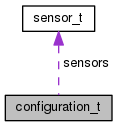
\includegraphics[width=160pt]{structconfiguration__t__coll__graph}
\end{center}
\end{figure}
\subsection*{Public Attributes}
\begin{DoxyCompactItemize}
\item 
\mbox{\Hypertarget{structconfiguration__t_a32d4c4bb78b5b231704c8a9f8d1b9e87}\label{structconfiguration__t_a32d4c4bb78b5b231704c8a9f8d1b9e87}} 
uint8\+\_\+t \hyperlink{structconfiguration__t_a32d4c4bb78b5b231704c8a9f8d1b9e87}{module\+\_\+version}
\begin{DoxyCompactList}\small\item\em module version \end{DoxyCompactList}\item 
\mbox{\Hypertarget{structconfiguration__t_a7dab895a0a9aa44bb65d90ef8016127d}\label{structconfiguration__t_a7dab895a0a9aa44bb65d90ef8016127d}} 
uint8\+\_\+t \hyperlink{structconfiguration__t_a7dab895a0a9aa44bb65d90ef8016127d}{module\+\_\+type}
\begin{DoxyCompactList}\small\item\em module type \end{DoxyCompactList}\item 
\mbox{\Hypertarget{structconfiguration__t_a0e088540266e347426ae73aed159f63a}\label{structconfiguration__t_a0e088540266e347426ae73aed159f63a}} 
uint8\+\_\+t \hyperlink{structconfiguration__t_a0e088540266e347426ae73aed159f63a}{i2c\+\_\+address}
\begin{DoxyCompactList}\small\item\em i2c address \end{DoxyCompactList}\item 
\mbox{\Hypertarget{structconfiguration__t_a227ef462f171f25e31cb3b0ce70b2597}\label{structconfiguration__t_a227ef462f171f25e31cb3b0ce70b2597}} 
bool \hyperlink{structconfiguration__t_a227ef462f171f25e31cb3b0ce70b2597}{is\+\_\+oneshot}
\begin{DoxyCompactList}\small\item\em enable or disable oneshot mode \end{DoxyCompactList}\item 
\mbox{\Hypertarget{structconfiguration__t_a33f99299576a58b3eb55be371e143531}\label{structconfiguration__t_a33f99299576a58b3eb55be371e143531}} 
bool \hyperlink{structconfiguration__t_a33f99299576a58b3eb55be371e143531}{is\+\_\+continuous}
\begin{DoxyCompactList}\small\item\em enable or disable continuous mode \end{DoxyCompactList}\item 
\mbox{\Hypertarget{structconfiguration__t_aed0a51c0dfbd925368c8539cf10c3001}\label{structconfiguration__t_aed0a51c0dfbd925368c8539cf10c3001}} 
uint8\+\_\+t \hyperlink{structconfiguration__t_aed0a51c0dfbd925368c8539cf10c3001}{i2c\+\_\+temperature\+\_\+address}
\begin{DoxyCompactList}\small\item\em i2c address of temperature sensor \end{DoxyCompactList}\item 
\mbox{\Hypertarget{structconfiguration__t_a79d1b1d9cb095c2bc0deb36c4f44452c}\label{structconfiguration__t_a79d1b1d9cb095c2bc0deb36c4f44452c}} 
uint8\+\_\+t \hyperlink{structconfiguration__t_a79d1b1d9cb095c2bc0deb36c4f44452c}{i2c\+\_\+humidity\+\_\+address}
\begin{DoxyCompactList}\small\item\em i2c address of humidity sensor \end{DoxyCompactList}\item 
\mbox{\Hypertarget{structconfiguration__t_aa003a99852a65bd2f9de0d230568bbbf}\label{structconfiguration__t_aa003a99852a65bd2f9de0d230568bbbf}} 
uint16\+\_\+t \hyperlink{structconfiguration__t_aa003a99852a65bd2f9de0d230568bbbf}{mqtt\+\_\+port}
\begin{DoxyCompactList}\small\item\em mqtt server port \end{DoxyCompactList}\item 
\mbox{\Hypertarget{structconfiguration__t_ad9a71a593cd2191ed132f9a2d6c00679}\label{structconfiguration__t_ad9a71a593cd2191ed132f9a2d6c00679}} 
char \hyperlink{structconfiguration__t_ad9a71a593cd2191ed132f9a2d6c00679}{mqtt\+\_\+server} \mbox{[}\hyperlink{mqtt__config_8h_a0a37bcf35cdbfc63d72beca198759c08}{M\+Q\+T\+T\+\_\+\+S\+E\+R\+V\+E\+R\+\_\+\+L\+E\+N\+G\+TH}\mbox{]}
\begin{DoxyCompactList}\small\item\em mqtt server \end{DoxyCompactList}\item 
\mbox{\Hypertarget{structconfiguration__t_acebf92623ad7bdf44f9707b0d99f50da}\label{structconfiguration__t_acebf92623ad7bdf44f9707b0d99f50da}} 
char \hyperlink{structconfiguration__t_acebf92623ad7bdf44f9707b0d99f50da}{mqtt\+\_\+root\+\_\+topic} \mbox{[}\hyperlink{mqtt__config_8h_a6d3b5b0f9c41b605e608f7d460491be6}{M\+Q\+T\+T\+\_\+\+R\+O\+O\+T\+\_\+\+T\+O\+P\+I\+C\+\_\+\+L\+E\+N\+G\+TH}\mbox{]}
\begin{DoxyCompactList}\small\item\em mqtt root path \end{DoxyCompactList}\item 
\mbox{\Hypertarget{structconfiguration__t_ae3699c4dd6979713472062bbad82c542}\label{structconfiguration__t_ae3699c4dd6979713472062bbad82c542}} 
char \hyperlink{structconfiguration__t_ae3699c4dd6979713472062bbad82c542}{mqtt\+\_\+subscribe\+\_\+topic} \mbox{[}\hyperlink{mqtt__config_8h_a2517f6560f7ee99813533e63d7fc91b6}{M\+Q\+T\+T\+\_\+\+S\+U\+B\+S\+C\+R\+I\+B\+E\+\_\+\+T\+O\+P\+I\+C\+\_\+\+L\+E\+N\+G\+TH}\mbox{]}
\begin{DoxyCompactList}\small\item\em mqtt subscribe topic \end{DoxyCompactList}\item 
\mbox{\Hypertarget{structconfiguration__t_ad97d47b585071f095a97296fc3e260e7}\label{structconfiguration__t_ad97d47b585071f095a97296fc3e260e7}} 
char \hyperlink{structconfiguration__t_ad97d47b585071f095a97296fc3e260e7}{mqtt\+\_\+username} \mbox{[}\hyperlink{mqtt__config_8h_a0e1860b8d036f571ffcb7e6d27832c16}{M\+Q\+T\+T\+\_\+\+U\+S\+E\+R\+N\+A\+M\+E\+\_\+\+L\+E\+N\+G\+TH}\mbox{]}
\begin{DoxyCompactList}\small\item\em mqtt username \end{DoxyCompactList}\item 
\mbox{\Hypertarget{structconfiguration__t_af842b7c625c3fdfb1b810e24fc1ba1b8}\label{structconfiguration__t_af842b7c625c3fdfb1b810e24fc1ba1b8}} 
char \hyperlink{structconfiguration__t_af842b7c625c3fdfb1b810e24fc1ba1b8}{mqtt\+\_\+password} \mbox{[}\hyperlink{mqtt__config_8h_a9fa040018ffd349e846cec27b2791fde}{M\+Q\+T\+T\+\_\+\+P\+A\+S\+S\+W\+O\+R\+D\+\_\+\+L\+E\+N\+G\+TH}\mbox{]}
\begin{DoxyCompactList}\small\item\em mqtt password \end{DoxyCompactList}\item 
\mbox{\Hypertarget{structconfiguration__t_a8de58dc10dfc6b369f34bae82426be5d}\label{structconfiguration__t_a8de58dc10dfc6b369f34bae82426be5d}} 
char \hyperlink{structconfiguration__t_a8de58dc10dfc6b369f34bae82426be5d}{ntp\+\_\+server} \mbox{[}\hyperlink{ntp__config_8h_a54153a6aa87c606f585ab167661b1be2}{N\+T\+P\+\_\+\+S\+E\+R\+V\+E\+R\+\_\+\+L\+E\+N\+G\+TH}\mbox{]}
\begin{DoxyCompactList}\small\item\em ntp server \end{DoxyCompactList}\item 
\mbox{\Hypertarget{structconfiguration__t_adede74f3da6d26f5bc4b5e64e4776f7f}\label{structconfiguration__t_adede74f3da6d26f5bc4b5e64e4776f7f}} 
\hyperlink{structsensor__t}{sensor\+\_\+t} \hyperlink{structconfiguration__t_adede74f3da6d26f5bc4b5e64e4776f7f}{sensors} \mbox{[}\hyperlink{rmap-config_8h_af18dc3de744722cb308451b7a705611b}{U\+S\+E\+\_\+\+S\+E\+N\+S\+O\+R\+S\+\_\+\+C\+O\+U\+NT}\mbox{]}
\begin{DoxyCompactList}\small\item\em \hyperlink{classSensorDriver}{Sensor\+Driver} buffer for storing sensors parameter. \end{DoxyCompactList}\item 
\mbox{\Hypertarget{structconfiguration__t_a9a1e7c702c2dd7270f31aca29264db86}\label{structconfiguration__t_a9a1e7c702c2dd7270f31aca29264db86}} 
uint8\+\_\+t \hyperlink{structconfiguration__t_a9a1e7c702c2dd7270f31aca29264db86}{sensors\+\_\+count}
\begin{DoxyCompactList}\small\item\em configured sensors number \end{DoxyCompactList}\item 
\mbox{\Hypertarget{structconfiguration__t_a0c0dc512cf86464d2e8dad486e042c5c}\label{structconfiguration__t_a0c0dc512cf86464d2e8dad486e042c5c}} 
uint16\+\_\+t \hyperlink{structconfiguration__t_a0c0dc512cf86464d2e8dad486e042c5c}{report\+\_\+seconds}
\begin{DoxyCompactList}\small\item\em seconds for report values \end{DoxyCompactList}\item 
\mbox{\Hypertarget{structconfiguration__t_a04554256dd43582433092cd70dd8b87d}\label{structconfiguration__t_a04554256dd43582433092cd70dd8b87d}} 
bool \hyperlink{structconfiguration__t_a04554256dd43582433092cd70dd8b87d}{is\+\_\+dhcp\+\_\+enable}
\begin{DoxyCompactList}\small\item\em dhcp status \end{DoxyCompactList}\item 
\mbox{\Hypertarget{structconfiguration__t_a6ade77826c87e62532cae8ca0f045dac}\label{structconfiguration__t_a6ade77826c87e62532cae8ca0f045dac}} 
uint8\+\_\+t \hyperlink{structconfiguration__t_a6ade77826c87e62532cae8ca0f045dac}{ethernet\+\_\+mac} \mbox{[}\hyperlink{ethernet__config_8h_aafad911924144dbfc03b66b146ed4439}{E\+T\+H\+E\+R\+N\+E\+T\+\_\+\+M\+A\+C\+\_\+\+L\+E\+N\+G\+TH}\mbox{]}
\begin{DoxyCompactList}\small\item\em ethernet mac \end{DoxyCompactList}\item 
\mbox{\Hypertarget{structconfiguration__t_a0b698acfbb52f889c906b9b175f7a5d5}\label{structconfiguration__t_a0b698acfbb52f889c906b9b175f7a5d5}} 
uint8\+\_\+t \hyperlink{structconfiguration__t_a0b698acfbb52f889c906b9b175f7a5d5}{ip} \mbox{[}\hyperlink{ethernet__config_8h_ae8de53528e88d8ff4516d82a48590bd7}{E\+T\+H\+E\+R\+N\+E\+T\+\_\+\+I\+P\+\_\+\+L\+E\+N\+G\+TH}\mbox{]}
\begin{DoxyCompactList}\small\item\em ip address \end{DoxyCompactList}\item 
\mbox{\Hypertarget{structconfiguration__t_a60716ed8c6a82119a46eb6345b88ca32}\label{structconfiguration__t_a60716ed8c6a82119a46eb6345b88ca32}} 
uint8\+\_\+t \hyperlink{structconfiguration__t_a60716ed8c6a82119a46eb6345b88ca32}{netmask} \mbox{[}\hyperlink{ethernet__config_8h_ae8de53528e88d8ff4516d82a48590bd7}{E\+T\+H\+E\+R\+N\+E\+T\+\_\+\+I\+P\+\_\+\+L\+E\+N\+G\+TH}\mbox{]}
\begin{DoxyCompactList}\small\item\em netmask \end{DoxyCompactList}\item 
\mbox{\Hypertarget{structconfiguration__t_a9d18b7f4094f4d7a50d2245e0370adc0}\label{structconfiguration__t_a9d18b7f4094f4d7a50d2245e0370adc0}} 
uint8\+\_\+t \hyperlink{structconfiguration__t_a9d18b7f4094f4d7a50d2245e0370adc0}{gateway} \mbox{[}\hyperlink{ethernet__config_8h_ae8de53528e88d8ff4516d82a48590bd7}{E\+T\+H\+E\+R\+N\+E\+T\+\_\+\+I\+P\+\_\+\+L\+E\+N\+G\+TH}\mbox{]}
\begin{DoxyCompactList}\small\item\em gateway \end{DoxyCompactList}\item 
\mbox{\Hypertarget{structconfiguration__t_acd481c434576a90959c342e877985b32}\label{structconfiguration__t_acd481c434576a90959c342e877985b32}} 
uint8\+\_\+t \hyperlink{structconfiguration__t_acd481c434576a90959c342e877985b32}{primary\+\_\+dns} \mbox{[}\hyperlink{ethernet__config_8h_ae8de53528e88d8ff4516d82a48590bd7}{E\+T\+H\+E\+R\+N\+E\+T\+\_\+\+I\+P\+\_\+\+L\+E\+N\+G\+TH}\mbox{]}
\begin{DoxyCompactList}\small\item\em primary dns \end{DoxyCompactList}\end{DoxyCompactItemize}


\subsection{Detailed Description}
E\+E\+P\+R\+OM saved configuration. 

The documentation for this struct was generated from the following files\+:\begin{DoxyCompactItemize}
\item 
sketchbook/rmap/i2c-\/rain/\hyperlink{i2c-rain_8h}{i2c-\/rain.\+h}\item 
sketchbook/rmap/i2c-\/th/\hyperlink{i2c-th_8h}{i2c-\/th.\+h}\item 
sketchbook/rmap/rmap/\hyperlink{rmap_8h}{rmap.\+h}\end{DoxyCompactItemize}

\chapter{File Documentation}
\hypertarget{rmap-config_8h}{}\section{rmap-\/config.h File Reference}
\label{rmap-config_8h}\index{rmap-\/config.\+h@{rmap-\/config.\+h}}
{\ttfamily \#include $<$stima\+\_\+module.\+h$>$}\newline
{\ttfamily \#include $<$sensors\+\_\+config.\+h$>$}\newline
Include dependency graph for rmap-\/config.h\+:
\nopagebreak
\begin{figure}[H]
\begin{center}
\leavevmode
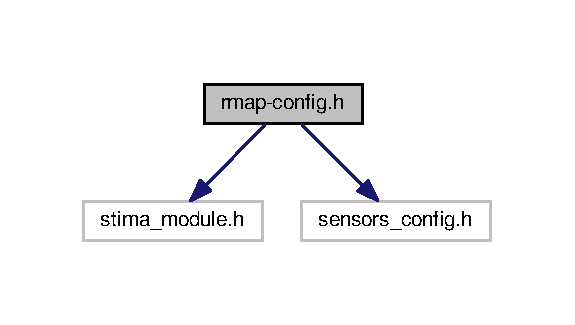
\includegraphics[width=276pt]{rmap-config_8h__incl}
\end{center}
\end{figure}
This graph shows which files directly or indirectly include this file\+:
\nopagebreak
\begin{figure}[H]
\begin{center}
\leavevmode
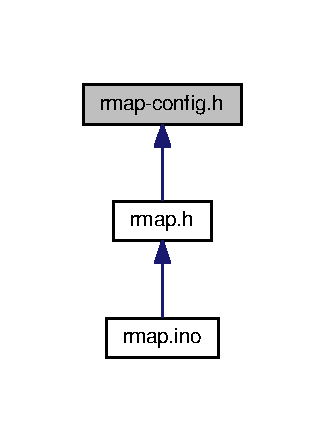
\includegraphics[width=156pt]{rmap-config_8h__dep__incl}
\end{center}
\end{figure}
\subsection*{Macros}
\begin{DoxyCompactItemize}
\item 
\mbox{\Hypertarget{rmap-config_8h_aa8639a8d4e83d9cc4187d7a751228464}\label{rmap-config_8h_aa8639a8d4e83d9cc4187d7a751228464}} 
\#define \hyperlink{rmap-config_8h_aa8639a8d4e83d9cc4187d7a751228464}{M\+O\+D\+U\+L\+E\+\_\+\+V\+E\+R\+S\+I\+ON}~(3)
\begin{DoxyCompactList}\small\item\em Module version. \end{DoxyCompactList}\item 
\mbox{\Hypertarget{rmap-config_8h_a8c815d03b3fd3e18ca06f920a1eb4e8e}\label{rmap-config_8h_a8c815d03b3fd3e18ca06f920a1eb4e8e}} 
\#define \hyperlink{rmap-config_8h_a8c815d03b3fd3e18ca06f920a1eb4e8e}{M\+O\+D\+U\+L\+E\+\_\+\+T\+Y\+PE}~(S\+T\+I\+M\+A\+\_\+\+M\+O\+D\+U\+L\+E\+\_\+\+T\+Y\+P\+E\+\_\+\+R\+E\+P\+O\+R\+T\+\_\+\+G\+SM)
\begin{DoxyCompactList}\small\item\em Type of module. It is defined in registers.\+h. \end{DoxyCompactList}\item 
\mbox{\Hypertarget{rmap-config_8h_a413cd84e34db40559ab834cc89408cdb}\label{rmap-config_8h_a413cd84e34db40559ab834cc89408cdb}} 
\#define \hyperlink{rmap-config_8h_a413cd84e34db40559ab834cc89408cdb}{C\+O\+N\+F\+I\+G\+U\+R\+A\+T\+I\+O\+N\+\_\+\+D\+E\+F\+A\+U\+L\+T\+\_\+\+T\+H\+\_\+\+A\+D\+D\+R\+E\+SS}~(I2\+C\+\_\+\+T\+H\+\_\+\+D\+E\+F\+A\+U\+L\+T\+\_\+\+A\+D\+D\+R\+E\+SS)
\begin{DoxyCompactList}\small\item\em Default i2c i2c-\/th address. \end{DoxyCompactList}\item 
\mbox{\Hypertarget{rmap-config_8h_a682b556c001cdf90f49b3a4d19081fb3}\label{rmap-config_8h_a682b556c001cdf90f49b3a4d19081fb3}} 
\#define \hyperlink{rmap-config_8h_a682b556c001cdf90f49b3a4d19081fb3}{C\+O\+N\+F\+I\+G\+U\+R\+A\+T\+I\+O\+N\+\_\+\+D\+E\+F\+A\+U\+L\+T\+\_\+\+R\+A\+I\+N\+\_\+\+A\+D\+D\+R\+E\+SS}~(I2\+C\+\_\+\+R\+A\+I\+N\+\_\+\+D\+E\+F\+A\+U\+L\+T\+\_\+\+A\+D\+D\+R\+E\+SS)
\begin{DoxyCompactList}\small\item\em Default i2c i2c-\/rain address. \end{DoxyCompactList}\item 
\mbox{\Hypertarget{rmap-config_8h_ae90da4786d4ba14563681879dba4d39c}\label{rmap-config_8h_ae90da4786d4ba14563681879dba4d39c}} 
\#define \hyperlink{rmap-config_8h_ae90da4786d4ba14563681879dba4d39c}{C\+O\+N\+F\+I\+G\+U\+R\+A\+T\+I\+O\+N\+\_\+\+R\+E\+S\+E\+T\+\_\+\+P\+IN}~(8)
\begin{DoxyCompactList}\small\item\em Input pin for reset configuration at startup. \end{DoxyCompactList}\item 
\mbox{\Hypertarget{rmap-config_8h_ad5f167ef5dab674e29cea328f672e0a3}\label{rmap-config_8h_ad5f167ef5dab674e29cea328f672e0a3}} 
\#define \hyperlink{rmap-config_8h_ad5f167ef5dab674e29cea328f672e0a3}{C\+O\+N\+F\+I\+G\+U\+R\+A\+T\+I\+O\+N\+\_\+\+D\+E\+F\+A\+U\+L\+T\+\_\+\+N\+T\+P\+\_\+\+S\+E\+R\+V\+ER}~(N\+T\+P\+\_\+\+D\+E\+F\+A\+U\+L\+T\+\_\+\+S\+E\+R\+V\+ER)
\begin{DoxyCompactList}\small\item\em Default ntp server. \end{DoxyCompactList}\item 
\mbox{\Hypertarget{rmap-config_8h_ab59fe331bcb2ec0b4c3abd6b13dc8c03}\label{rmap-config_8h_ab59fe331bcb2ec0b4c3abd6b13dc8c03}} 
\#define \hyperlink{rmap-config_8h_ab59fe331bcb2ec0b4c3abd6b13dc8c03}{C\+O\+N\+F\+I\+G\+U\+R\+A\+T\+I\+O\+N\+\_\+\+D\+E\+F\+A\+U\+L\+T\+\_\+\+M\+Q\+T\+T\+\_\+\+P\+O\+RT}~(M\+Q\+T\+T\+\_\+\+D\+E\+F\+A\+U\+L\+T\+\_\+\+P\+O\+RT)
\begin{DoxyCompactList}\small\item\em Default mqtt server port. \end{DoxyCompactList}\item 
\mbox{\Hypertarget{rmap-config_8h_aec48aba6054d0eab8b9d9fb857f2a33c}\label{rmap-config_8h_aec48aba6054d0eab8b9d9fb857f2a33c}} 
\#define \hyperlink{rmap-config_8h_aec48aba6054d0eab8b9d9fb857f2a33c}{C\+O\+N\+F\+I\+G\+U\+R\+A\+T\+I\+O\+N\+\_\+\+D\+E\+F\+A\+U\+L\+T\+\_\+\+M\+Q\+T\+T\+\_\+\+S\+E\+R\+V\+ER}~(M\+Q\+T\+T\+\_\+\+D\+E\+F\+A\+U\+L\+T\+\_\+\+S\+E\+R\+V\+ER)
\begin{DoxyCompactList}\small\item\em Default mqtt server. \end{DoxyCompactList}\item 
\mbox{\Hypertarget{rmap-config_8h_a85521de6b08f8704bd35a8e34edef4f8}\label{rmap-config_8h_a85521de6b08f8704bd35a8e34edef4f8}} 
\#define \hyperlink{rmap-config_8h_a85521de6b08f8704bd35a8e34edef4f8}{C\+O\+N\+F\+I\+G\+U\+R\+A\+T\+I\+O\+N\+\_\+\+D\+E\+F\+A\+U\+L\+T\+\_\+\+M\+Q\+T\+T\+\_\+\+R\+O\+O\+T\+\_\+\+T\+O\+P\+IC}~(M\+Q\+T\+T\+\_\+\+D\+E\+F\+A\+U\+L\+T\+\_\+\+R\+O\+O\+T\+\_\+\+T\+O\+P\+IC)
\begin{DoxyCompactList}\small\item\em Default mqtt root topic. \end{DoxyCompactList}\item 
\mbox{\Hypertarget{rmap-config_8h_ad5f5c2f91406f76021e58aaebb4fe84d}\label{rmap-config_8h_ad5f5c2f91406f76021e58aaebb4fe84d}} 
\#define \hyperlink{rmap-config_8h_ad5f5c2f91406f76021e58aaebb4fe84d}{C\+O\+N\+F\+I\+G\+U\+R\+A\+T\+I\+O\+N\+\_\+\+D\+E\+F\+A\+U\+L\+T\+\_\+\+M\+Q\+T\+T\+\_\+\+S\+U\+B\+S\+C\+R\+I\+B\+E\+\_\+\+T\+O\+P\+IC}~(M\+Q\+T\+T\+\_\+\+D\+E\+F\+A\+U\+L\+T\+\_\+\+S\+U\+B\+S\+C\+R\+I\+B\+E\+\_\+\+T\+O\+P\+IC)
\begin{DoxyCompactList}\small\item\em Default mqtt subscribe topic. \end{DoxyCompactList}\item 
\mbox{\Hypertarget{rmap-config_8h_a4606b704d26885b00b68c8e7d1c4b77a}\label{rmap-config_8h_a4606b704d26885b00b68c8e7d1c4b77a}} 
\#define \hyperlink{rmap-config_8h_a4606b704d26885b00b68c8e7d1c4b77a}{C\+O\+N\+F\+I\+G\+U\+R\+A\+T\+I\+O\+N\+\_\+\+D\+E\+F\+A\+U\+L\+T\+\_\+\+M\+Q\+T\+T\+\_\+\+U\+S\+E\+R\+N\+A\+ME}~(M\+Q\+T\+T\+\_\+\+D\+E\+F\+A\+U\+L\+T\+\_\+\+U\+S\+E\+R\+N\+A\+ME)
\begin{DoxyCompactList}\small\item\em Default mqtt username. \end{DoxyCompactList}\item 
\mbox{\Hypertarget{rmap-config_8h_a93f4ec08026dd0e8eaffc77a72986283}\label{rmap-config_8h_a93f4ec08026dd0e8eaffc77a72986283}} 
\#define \hyperlink{rmap-config_8h_a93f4ec08026dd0e8eaffc77a72986283}{C\+O\+N\+F\+I\+G\+U\+R\+A\+T\+I\+O\+N\+\_\+\+D\+E\+F\+A\+U\+L\+T\+\_\+\+M\+Q\+T\+T\+\_\+\+P\+A\+S\+S\+W\+O\+RD}~(M\+Q\+T\+T\+\_\+\+D\+E\+F\+A\+U\+L\+T\+\_\+\+P\+A\+S\+S\+W\+O\+RD)
\begin{DoxyCompactList}\small\item\em Default mqtt password. \end{DoxyCompactList}\item 
\mbox{\Hypertarget{rmap-config_8h_aedfe334cb469b9ad487a0ba637d29662}\label{rmap-config_8h_aedfe334cb469b9ad487a0ba637d29662}} 
\#define \hyperlink{rmap-config_8h_aedfe334cb469b9ad487a0ba637d29662}{C\+O\+N\+F\+I\+G\+U\+R\+A\+T\+I\+O\+N\+\_\+\+D\+E\+F\+A\+U\+L\+T\+\_\+\+E\+T\+H\+E\+R\+N\+E\+T\+\_\+\+D\+H\+C\+P\+\_\+\+E\+N\+A\+B\+LE}~(E\+T\+H\+E\+R\+N\+E\+T\+\_\+\+D\+E\+F\+A\+U\+L\+T\+\_\+\+D\+H\+C\+P\+\_\+\+E\+N\+A\+B\+LE)
\begin{DoxyCompactList}\small\item\em Default D\+H\+CP status. \end{DoxyCompactList}\item 
\mbox{\Hypertarget{rmap-config_8h_a5333d2c3bcda84cc19a56f3ab7a2bcce}\label{rmap-config_8h_a5333d2c3bcda84cc19a56f3ab7a2bcce}} 
\#define \hyperlink{rmap-config_8h_a5333d2c3bcda84cc19a56f3ab7a2bcce}{C\+O\+N\+F\+I\+G\+U\+R\+A\+T\+I\+O\+N\+\_\+\+D\+E\+F\+A\+U\+L\+T\+\_\+\+E\+T\+H\+E\+R\+N\+E\+T\+\_\+\+M\+AC}~(E\+T\+H\+E\+R\+N\+E\+T\+\_\+\+D\+E\+F\+A\+U\+L\+T\+\_\+\+M\+AC)
\begin{DoxyCompactList}\small\item\em Default mac address. \end{DoxyCompactList}\item 
\mbox{\Hypertarget{rmap-config_8h_ae03d41374839792a8b5585ebf9bdcd3b}\label{rmap-config_8h_ae03d41374839792a8b5585ebf9bdcd3b}} 
\#define \hyperlink{rmap-config_8h_ae03d41374839792a8b5585ebf9bdcd3b}{C\+O\+N\+F\+I\+G\+U\+R\+A\+T\+I\+O\+N\+\_\+\+D\+E\+F\+A\+U\+L\+T\+\_\+\+E\+T\+H\+E\+R\+N\+E\+T\+\_\+\+IP}~(E\+T\+H\+E\+R\+N\+E\+T\+\_\+\+D\+E\+F\+A\+U\+L\+T\+\_\+\+IP)
\begin{DoxyCompactList}\small\item\em Default ip address. \end{DoxyCompactList}\item 
\mbox{\Hypertarget{rmap-config_8h_a6e0029e4ba852ab74d69263d934c7160}\label{rmap-config_8h_a6e0029e4ba852ab74d69263d934c7160}} 
\#define \hyperlink{rmap-config_8h_a6e0029e4ba852ab74d69263d934c7160}{C\+O\+N\+F\+I\+G\+U\+R\+A\+T\+I\+O\+N\+\_\+\+D\+E\+F\+A\+U\+L\+T\+\_\+\+E\+T\+H\+E\+R\+N\+E\+T\+\_\+\+N\+E\+T\+M\+A\+SK}~(E\+T\+H\+E\+R\+N\+E\+T\+\_\+\+D\+E\+F\+A\+U\+L\+T\+\_\+\+N\+E\+T\+M\+A\+SK)
\begin{DoxyCompactList}\small\item\em Default netmask address. \end{DoxyCompactList}\item 
\mbox{\Hypertarget{rmap-config_8h_adb31ecf5d2e45dab1b0508a21313267b}\label{rmap-config_8h_adb31ecf5d2e45dab1b0508a21313267b}} 
\#define \hyperlink{rmap-config_8h_adb31ecf5d2e45dab1b0508a21313267b}{C\+O\+N\+F\+I\+G\+U\+R\+A\+T\+I\+O\+N\+\_\+\+D\+E\+F\+A\+U\+L\+T\+\_\+\+E\+T\+H\+E\+R\+N\+E\+T\+\_\+\+G\+A\+T\+E\+W\+AY}~(E\+T\+H\+E\+R\+N\+E\+T\+\_\+\+D\+E\+F\+A\+U\+L\+T\+\_\+\+G\+A\+T\+E\+W\+AY)
\begin{DoxyCompactList}\small\item\em Default gateway address. \end{DoxyCompactList}\item 
\mbox{\Hypertarget{rmap-config_8h_a7e0faf050a00ee299bd47f28d9b38c63}\label{rmap-config_8h_a7e0faf050a00ee299bd47f28d9b38c63}} 
\#define \hyperlink{rmap-config_8h_a7e0faf050a00ee299bd47f28d9b38c63}{C\+O\+N\+F\+I\+G\+U\+R\+A\+T\+I\+O\+N\+\_\+\+D\+E\+F\+A\+U\+L\+T\+\_\+\+E\+T\+H\+E\+R\+N\+E\+T\+\_\+\+P\+R\+I\+M\+A\+R\+Y\+\_\+\+D\+NS}~(E\+T\+H\+E\+R\+N\+E\+T\+\_\+\+D\+E\+F\+A\+U\+L\+T\+\_\+\+P\+R\+I\+M\+A\+R\+Y\+\_\+\+D\+NS)
\begin{DoxyCompactList}\small\item\em Default primary dns address. \end{DoxyCompactList}\item 
\mbox{\Hypertarget{rmap-config_8h_a9ace81994cbeb6153f9dd5adf0e6dbee}\label{rmap-config_8h_a9ace81994cbeb6153f9dd5adf0e6dbee}} 
\#define \hyperlink{rmap-config_8h_a9ace81994cbeb6153f9dd5adf0e6dbee}{U\+S\+E\+\_\+\+P\+O\+W\+E\+R\+\_\+\+D\+O\+WN}~(false)
\begin{DoxyCompactList}\small\item\em Enable or disable power down. \end{DoxyCompactList}\item 
\mbox{\Hypertarget{rmap-config_8h_a7b9497e328b8f872cd7677cfd02bbf65}\label{rmap-config_8h_a7b9497e328b8f872cd7677cfd02bbf65}} 
\#define \hyperlink{rmap-config_8h_a7b9497e328b8f872cd7677cfd02bbf65}{D\+E\+B\+O\+U\+N\+C\+I\+N\+G\+\_\+\+P\+O\+W\+E\+R\+\_\+\+D\+O\+W\+N\+\_\+\+T\+I\+M\+E\+\_\+\+MS}~(10)
\begin{DoxyCompactList}\small\item\em Debounce power down ms. \end{DoxyCompactList}\item 
\mbox{\Hypertarget{rmap-config_8h_a8051c2a569a9f9c488af89bce47ec306}\label{rmap-config_8h_a8051c2a569a9f9c488af89bce47ec306}} 
\#define \hyperlink{rmap-config_8h_a8051c2a569a9f9c488af89bce47ec306}{U\+S\+E\+\_\+\+T\+I\+M\+E\+R\+\_\+1}~(false)
\begin{DoxyCompactList}\small\item\em Enable or disable timer1. \end{DoxyCompactList}\item 
\mbox{\Hypertarget{rmap-config_8h_a487cf0916151ca6772bc10ad17de96f8}\label{rmap-config_8h_a487cf0916151ca6772bc10ad17de96f8}} 
\#define \hyperlink{rmap-config_8h_a487cf0916151ca6772bc10ad17de96f8}{W5500\+\_\+\+C\+H\+I\+P\+\_\+\+S\+E\+L\+E\+C\+T\+\_\+\+P\+IN}~(10)
\begin{DoxyCompactList}\small\item\em Chip select pin for Wiznet W5500 ethernet module. \end{DoxyCompactList}\item 
\mbox{\Hypertarget{rmap-config_8h_a52845a6b315de684e7eda2ffe7863b55}\label{rmap-config_8h_a52845a6b315de684e7eda2ffe7863b55}} 
\#define \hyperlink{rmap-config_8h_a52845a6b315de684e7eda2ffe7863b55}{S\+D\+C\+A\+R\+D\+\_\+\+C\+H\+I\+P\+\_\+\+S\+E\+L\+E\+C\+T\+\_\+\+P\+IN}~(7)
\begin{DoxyCompactList}\small\item\em Chip select pin for S\+D-\/\+Card module. \end{DoxyCompactList}\item 
\#define \hyperlink{rmap-config_8h_a983c9777673ee873f12ec9f489215321}{W\+D\+T\+\_\+\+T\+I\+M\+ER}~(W\+D\+T\+O\+\_\+8S)
\begin{DoxyCompactList}\small\item\em Watchdog timer for periodically check microprocessor block states. \end{DoxyCompactList}\item 
\mbox{\Hypertarget{rmap-config_8h_a6b7af814754ac70e8aa5e34aa9295df5}\label{rmap-config_8h_a6b7af814754ac70e8aa5e34aa9295df5}} 
\#define \hyperlink{rmap-config_8h_a6b7af814754ac70e8aa5e34aa9295df5}{R\+T\+C\+\_\+\+F\+R\+E\+Q\+U\+E\+N\+CY}~(P\+C\+F8563\+\_\+\+C\+L\+K\+O\+U\+T\+\_\+\+F\+R\+E\+Q\+U\+E\+N\+C\+Y\+\_\+\+S\+E\+C\+O\+N\+DS)
\begin{DoxyCompactList}\small\item\em Real time clock frequency for generating interrupt for awaken the microprocessor and execute timed tasks. \end{DoxyCompactList}\item 
\mbox{\Hypertarget{rmap-config_8h_a1efb928882c9a9d83d78e499091a8319}\label{rmap-config_8h_a1efb928882c9a9d83d78e499091a8319}} 
\#define \hyperlink{rmap-config_8h_a1efb928882c9a9d83d78e499091a8319}{R\+T\+C\+\_\+\+I\+N\+T\+E\+R\+R\+U\+P\+T\+\_\+\+P\+IN}~(6)
\begin{DoxyCompactList}\small\item\em Interrupt pin for rtc. \end{DoxyCompactList}\item 
\mbox{\Hypertarget{rmap-config_8h_af18dc3de744722cb308451b7a705611b}\label{rmap-config_8h_af18dc3de744722cb308451b7a705611b}} 
\#define \hyperlink{rmap-config_8h_af18dc3de744722cb308451b7a705611b}{U\+S\+E\+\_\+\+S\+E\+N\+S\+O\+R\+S\+\_\+\+C\+O\+U\+NT}~(U\+S\+E\+\_\+\+S\+E\+N\+S\+O\+R\+\_\+\+I\+TH + U\+S\+E\+\_\+\+S\+E\+N\+S\+O\+R\+\_\+\+M\+TH + U\+S\+E\+\_\+\+S\+E\+N\+S\+O\+R\+\_\+\+N\+TH + U\+S\+E\+\_\+\+S\+E\+N\+S\+O\+R\+\_\+\+X\+TH + U\+S\+E\+\_\+\+S\+E\+N\+S\+O\+R\+\_\+\+T\+BS + U\+S\+E\+\_\+\+S\+E\+N\+S\+O\+R\+\_\+\+T\+BR + U\+S\+E\+\_\+\+S\+E\+N\+S\+O\+R\+\_\+\+D\+EP)
\begin{DoxyCompactList}\small\item\em Sensors count. \end{DoxyCompactList}\item 
\mbox{\Hypertarget{rmap-config_8h_a16fa5577ef44bb1146f17a3bc43194b1}\label{rmap-config_8h_a16fa5577ef44bb1146f17a3bc43194b1}} 
\#define \hyperlink{rmap-config_8h_a16fa5577ef44bb1146f17a3bc43194b1}{S\+E\+N\+S\+O\+R\+S\+\_\+\+R\+E\+T\+R\+Y\+\_\+\+C\+O\+U\+N\+T\+\_\+\+M\+AX}~(3)
\begin{DoxyCompactList}\small\item\em Maximum number of retry for sensors reading. \end{DoxyCompactList}\item 
\mbox{\Hypertarget{rmap-config_8h_a8ea8eeea7855628652f697bab3d173b5}\label{rmap-config_8h_a8ea8eeea7855628652f697bab3d173b5}} 
\#define \hyperlink{rmap-config_8h_a8ea8eeea7855628652f697bab3d173b5}{S\+E\+N\+S\+O\+R\+S\+\_\+\+R\+E\+T\+R\+Y\+\_\+\+D\+E\+L\+A\+Y\+\_\+\+MS}~(50)
\begin{DoxyCompactList}\small\item\em Waiting for reading between two attempts. \end{DoxyCompactList}\item 
\mbox{\Hypertarget{rmap-config_8h_a7e36149c4e27cedef72823f8212b4fea}\label{rmap-config_8h_a7e36149c4e27cedef72823f8212b4fea}} 
\#define \hyperlink{rmap-config_8h_a7e36149c4e27cedef72823f8212b4fea}{D\+A\+T\+A\+\_\+\+P\+R\+O\+C\+E\+S\+S\+I\+N\+G\+\_\+\+R\+E\+T\+R\+Y\+\_\+\+C\+O\+U\+N\+T\+\_\+\+M\+AX}~(2)
\begin{DoxyCompactList}\small\item\em Maximum number of retry for processing acquired data. \end{DoxyCompactList}\item 
\mbox{\Hypertarget{rmap-config_8h_a2933698b1b2aa94bf5755a89efbd05f7}\label{rmap-config_8h_a2933698b1b2aa94bf5755a89efbd05f7}} 
\#define \hyperlink{rmap-config_8h_a2933698b1b2aa94bf5755a89efbd05f7}{D\+A\+T\+A\+\_\+\+P\+R\+O\+C\+E\+S\+S\+I\+N\+G\+\_\+\+R\+E\+T\+R\+Y\+\_\+\+D\+E\+L\+A\+Y\+\_\+\+MS}~(500)
\begin{DoxyCompactList}\small\item\em Wait time between two attempts. \end{DoxyCompactList}\item 
\mbox{\Hypertarget{rmap-config_8h_a81ed8eac7c6867ba31602628402f97c1}\label{rmap-config_8h_a81ed8eac7c6867ba31602628402f97c1}} 
\#define \hyperlink{rmap-config_8h_a81ed8eac7c6867ba31602628402f97c1}{D\+A\+T\+A\+\_\+\+S\+A\+V\+I\+N\+G\+\_\+\+R\+E\+T\+R\+Y\+\_\+\+C\+O\+U\+N\+T\+\_\+\+M\+AX}~(3)
\begin{DoxyCompactList}\small\item\em Maximum number of retry for saving data on S\+D-\/\+Card. \end{DoxyCompactList}\item 
\mbox{\Hypertarget{rmap-config_8h_a511bba65f6e387335efa4c2ca6a9d948}\label{rmap-config_8h_a511bba65f6e387335efa4c2ca6a9d948}} 
\#define \hyperlink{rmap-config_8h_a511bba65f6e387335efa4c2ca6a9d948}{D\+A\+T\+A\+\_\+\+S\+A\+V\+I\+N\+G\+\_\+\+D\+E\+L\+A\+Y\+\_\+\+MS}~(1000)
\begin{DoxyCompactList}\small\item\em Wait time between two attempts. \end{DoxyCompactList}\item 
\mbox{\Hypertarget{rmap-config_8h_a823e4d8bca9ba0990f5c085dc997fafb}\label{rmap-config_8h_a823e4d8bca9ba0990f5c085dc997fafb}} 
\#define \hyperlink{rmap-config_8h_a823e4d8bca9ba0990f5c085dc997fafb}{M\+Q\+T\+T\+\_\+\+R\+E\+T\+R\+Y\+\_\+\+C\+O\+U\+N\+T\+\_\+\+M\+AX}~(3)
\begin{DoxyCompactList}\small\item\em Maximum number of retry for doing mqtt operations. \end{DoxyCompactList}\item 
\mbox{\Hypertarget{rmap-config_8h_a4a9d04eab0c57e3143a6d1be60b73fb3}\label{rmap-config_8h_a4a9d04eab0c57e3143a6d1be60b73fb3}} 
\#define \hyperlink{rmap-config_8h_a4a9d04eab0c57e3143a6d1be60b73fb3}{M\+Q\+T\+T\+\_\+\+D\+E\+L\+A\+Y\+\_\+\+MS}~(1000)
\begin{DoxyCompactList}\small\item\em Wait time between two attempts. \end{DoxyCompactList}\item 
\mbox{\Hypertarget{rmap-config_8h_a578ee6f26618a9f795fb5828663431f0}\label{rmap-config_8h_a578ee6f26618a9f795fb5828663431f0}} 
\#define \hyperlink{rmap-config_8h_a578ee6f26618a9f795fb5828663431f0}{I\+P\+\_\+\+S\+T\+A\+C\+K\+\_\+\+T\+I\+M\+E\+O\+U\+T\+\_\+\+MS}~(M\+Q\+T\+T\+\_\+\+T\+I\+M\+E\+O\+U\+T\+\_\+\+MS)
\begin{DoxyCompactList}\small\item\em I\+P\+Stack timeout. \end{DoxyCompactList}\item 
\mbox{\Hypertarget{rmap-config_8h_a7ac76db6c397b6167fb6dc9f4c88d6f3}\label{rmap-config_8h_a7ac76db6c397b6167fb6dc9f4c88d6f3}} 
\#define \hyperlink{rmap-config_8h_a7ac76db6c397b6167fb6dc9f4c88d6f3}{S\+U\+P\+E\+R\+V\+I\+S\+O\+R\+\_\+\+C\+O\+N\+N\+E\+C\+T\+I\+O\+N\+\_\+\+L\+E\+V\+E\+L\+\_\+\+R\+E\+T\+R\+Y\+\_\+\+C\+O\+U\+N\+T\+\_\+\+M\+AX}~(5)
\begin{DoxyCompactList}\small\item\em Maximum number of retry for doing supervisor operations. \end{DoxyCompactList}\item 
\mbox{\Hypertarget{rmap-config_8h_a52ca4538c4f04d08d9b1f35329926912}\label{rmap-config_8h_a52ca4538c4f04d08d9b1f35329926912}} 
\#define \hyperlink{rmap-config_8h_a52ca4538c4f04d08d9b1f35329926912}{S\+U\+P\+E\+R\+V\+I\+S\+O\+R\+\_\+\+C\+O\+N\+N\+E\+C\+T\+I\+O\+N\+\_\+\+T\+I\+M\+E\+O\+U\+T\+\_\+\+MS}~(120000)
\begin{DoxyCompactList}\small\item\em Timeout for connecting. \end{DoxyCompactList}\item 
\mbox{\Hypertarget{rmap-config_8h_aa5742869009a8ff3a6e3dfcb700f3ab6}\label{rmap-config_8h_aa5742869009a8ff3a6e3dfcb700f3ab6}} 
\#define \hyperlink{rmap-config_8h_aa5742869009a8ff3a6e3dfcb700f3ab6}{S\+T\+R\+E\+A\+M\+\_\+\+U\+A\+R\+T\+\_\+\+S\+T\+R\+E\+A\+M\+\_\+\+T\+I\+M\+E\+O\+U\+T\+\_\+\+MS}~(5)
\begin{DoxyCompactList}\small\item\em Timeout for receiving next byte from stream. \end{DoxyCompactList}\item 
\mbox{\Hypertarget{rmap-config_8h_a950ba415f1afc5bdc2d4ea52b51075df}\label{rmap-config_8h_a950ba415f1afc5bdc2d4ea52b51075df}} 
\#define \hyperlink{rmap-config_8h_a950ba415f1afc5bdc2d4ea52b51075df}{S\+T\+R\+E\+A\+M\+\_\+\+U\+A\+R\+T\+\_\+\+S\+T\+R\+E\+A\+M\+\_\+\+E\+N\+D\+\_\+\+T\+I\+M\+E\+O\+U\+T\+\_\+\+MS}~(10000)
\begin{DoxyCompactList}\small\item\em Timeout for close stream after last received byte. \end{DoxyCompactList}\item 
\mbox{\Hypertarget{rmap-config_8h_ac5fc989b784c420be7db4f66417fc744}\label{rmap-config_8h_ac5fc989b784c420be7db4f66417fc744}} 
\#define \hyperlink{rmap-config_8h_ac5fc989b784c420be7db4f66417fc744}{S\+T\+R\+E\+A\+M\+\_\+\+B\+U\+F\+F\+E\+R\+\_\+\+L\+E\+N\+G\+TH}~(192)
\begin{DoxyCompactList}\small\item\em Stream buffer length. \end{DoxyCompactList}\item 
\mbox{\Hypertarget{rmap-config_8h_a7470ca0f869e88a49d4d70bad5de69e6}\label{rmap-config_8h_a7470ca0f869e88a49d4d70bad5de69e6}} 
\#define \hyperlink{rmap-config_8h_a7470ca0f869e88a49d4d70bad5de69e6}{S\+D\+C\+A\+R\+D\+\_\+\+M\+Q\+T\+T\+\_\+\+P\+T\+R\+\_\+\+F\+I\+L\+E\+\_\+\+N\+A\+ME}~(\char`\"{}mqtt\+\_\+ptr.\+txt\char`\"{})
\begin{DoxyCompactList}\small\item\em Data file on S\+D-\/\+Card containing the pointer to the last mqtt transmitted data. \end{DoxyCompactList}\item 
\mbox{\Hypertarget{rmap-config_8h_a5042473c874b6f184bd4dc197feadca9}\label{rmap-config_8h_a5042473c874b6f184bd4dc197feadca9}} 
\#define \hyperlink{rmap-config_8h_a5042473c874b6f184bd4dc197feadca9}{N\+T\+P\+\_\+\+R\+E\+T\+R\+Y\+\_\+\+C\+O\+U\+N\+T\+\_\+\+M\+AX}~(5)
\begin{DoxyCompactList}\small\item\em Maximum number of retry for doing ntp operations. \end{DoxyCompactList}\item 
\mbox{\Hypertarget{rmap-config_8h_aee0934e91270bda3cc3fcaa9082fadc8}\label{rmap-config_8h_aee0934e91270bda3cc3fcaa9082fadc8}} 
\#define \hyperlink{rmap-config_8h_aee0934e91270bda3cc3fcaa9082fadc8}{N\+T\+P\+\_\+\+R\+E\+T\+R\+Y\+\_\+\+D\+E\+L\+A\+Y\+\_\+\+MS}~(100)
\begin{DoxyCompactList}\small\item\em Wait time between two attempts. \end{DoxyCompactList}\item 
\mbox{\Hypertarget{rmap-config_8h_ac26c9e27fc41a5f7c43968b47b2d8cfc}\label{rmap-config_8h_ac26c9e27fc41a5f7c43968b47b2d8cfc}} 
\#define \hyperlink{rmap-config_8h_ac26c9e27fc41a5f7c43968b47b2d8cfc}{N\+T\+P\+\_\+\+T\+I\+M\+E\+\_\+\+F\+O\+R\+\_\+\+R\+E\+S\+Y\+N\+C\+\_\+S}~(S\+E\+C\+S\+\_\+\+P\+E\+R\+\_\+\+D\+AY)
\begin{DoxyCompactList}\small\item\em Maximum seconds for resync time over ntp. \end{DoxyCompactList}\item 
\mbox{\Hypertarget{rmap-config_8h_af546d356bff5c682bba4aeeed199d5df}\label{rmap-config_8h_af546d356bff5c682bba4aeeed199d5df}} 
\#define \hyperlink{rmap-config_8h_af546d356bff5c682bba4aeeed199d5df}{L\+C\+D\+\_\+\+T\+I\+M\+E\+\_\+\+F\+O\+R\+\_\+\+R\+E\+I\+N\+I\+T\+I\+A\+L\+I\+Z\+E\+\_\+S}~(S\+E\+C\+S\+\_\+\+P\+E\+R\+\_\+\+H\+O\+UR)
\begin{DoxyCompactList}\small\item\em Maximum seconds for reinitialize L\+CD. \end{DoxyCompactList}\item 
\mbox{\Hypertarget{rmap-config_8h_ab5d88aab471d5cac3392cae63b8684cf}\label{rmap-config_8h_ab5d88aab471d5cac3392cae63b8684cf}} 
\#define \hyperlink{rmap-config_8h_ab5d88aab471d5cac3392cae63b8684cf}{T\+I\+M\+E\+\_\+\+R\+E\+S\+Y\+N\+C\+\_\+\+I\+N\+T\+E\+R\+V\+A\+L\+S\+\_\+S}~(S\+E\+C\+S\+\_\+\+P\+E\+R\+\_\+\+W\+E\+EK)
\begin{DoxyCompactList}\small\item\em Interval in seconds for resync time. \end{DoxyCompactList}\item 
\mbox{\Hypertarget{rmap-config_8h_a743e7905c81f2b5b6bb32fc55a3c5494}\label{rmap-config_8h_a743e7905c81f2b5b6bb32fc55a3c5494}} 
\#define \hyperlink{rmap-config_8h_a743e7905c81f2b5b6bb32fc55a3c5494}{E\+T\+H\+E\+R\+N\+E\+T\+\_\+\+R\+E\+T\+R\+Y\+\_\+\+C\+O\+U\+N\+T\+\_\+\+M\+AX}~(5)
\begin{DoxyCompactList}\small\item\em Maximum number of retry for doing ethernet operations. \end{DoxyCompactList}\item 
\mbox{\Hypertarget{rmap-config_8h_aad84a5cc78471bbe08ae9b0f519866ea}\label{rmap-config_8h_aad84a5cc78471bbe08ae9b0f519866ea}} 
\#define \hyperlink{rmap-config_8h_aad84a5cc78471bbe08ae9b0f519866ea}{E\+T\+H\+E\+R\+N\+E\+T\+\_\+\+R\+E\+T\+R\+Y\+\_\+\+D\+E\+L\+A\+Y\+\_\+\+MS}~(E\+T\+H\+E\+R\+N\+E\+T\+\_\+\+A\+T\+T\+E\+M\+P\+T\+\_\+\+MS)
\begin{DoxyCompactList}\small\item\em Wait time between two attempts. \end{DoxyCompactList}\end{DoxyCompactItemize}


\subsection{Macro Definition Documentation}
\mbox{\Hypertarget{rmap-config_8h_a983c9777673ee873f12ec9f489215321}\label{rmap-config_8h_a983c9777673ee873f12ec9f489215321}} 
\index{rmap-\/config.\+h@{rmap-\/config.\+h}!W\+D\+T\+\_\+\+T\+I\+M\+ER@{W\+D\+T\+\_\+\+T\+I\+M\+ER}}
\index{W\+D\+T\+\_\+\+T\+I\+M\+ER@{W\+D\+T\+\_\+\+T\+I\+M\+ER}!rmap-\/config.\+h@{rmap-\/config.\+h}}
\subsubsection{\texorpdfstring{W\+D\+T\+\_\+\+T\+I\+M\+ER}{WDT\_TIMER}}
{\footnotesize\ttfamily \#define W\+D\+T\+\_\+\+T\+I\+M\+ER~(W\+D\+T\+O\+\_\+8S)}



Watchdog timer for periodically check microprocessor block states. 

Possible value for W\+D\+T\+\_\+\+T\+I\+M\+ER are\+: W\+D\+T\+O\+\_\+15\+MS, W\+D\+T\+O\+\_\+30\+MS, W\+D\+T\+O\+\_\+60\+MS, W\+D\+T\+O\+\_\+120\+MS, W\+D\+T\+O\+\_\+250\+MS, W\+D\+T\+O\+\_\+500\+MS, W\+D\+T\+O\+\_\+1S, W\+D\+T\+O\+\_\+2S, W\+D\+T\+O\+\_\+4S, W\+D\+T\+O\+\_\+8S 
\hypertarget{rmap_8h}{}\section{sketchbook/rmap/rmap/rmap.h File Reference}
\label{rmap_8h}\index{sketchbook/rmap/rmap/rmap.\+h@{sketchbook/rmap/rmap/rmap.\+h}}
{\ttfamily \#include \char`\"{}rmap-\/config.\+h\char`\"{}}\newline
{\ttfamily \#include $<$typedef.\+h$>$}\newline
{\ttfamily \#include $<$debug.\+h$>$}\newline
{\ttfamily \#include $<$hardware\+\_\+config.\+h$>$}\newline
{\ttfamily \#include $<$json\+\_\+config.\+h$>$}\newline
{\ttfamily \#include $<$ntp\+\_\+config.\+h$>$}\newline
{\ttfamily \#include $<$lcd\+\_\+config.\+h$>$}\newline
{\ttfamily \#include $<$avr/sleep.\+h$>$}\newline
{\ttfamily \#include $<$avr/power.\+h$>$}\newline
{\ttfamily \#include $<$avr/wdt.\+h$>$}\newline
{\ttfamily \#include $<$S\+P\+I.\+h$>$}\newline
{\ttfamily \#include $<$Wire.\+h$>$}\newline
{\ttfamily \#include $<$Sd\+Fat.\+h$>$}\newline
{\ttfamily \#include $<$pcf8563.\+h$>$}\newline
{\ttfamily \#include $<$ntp.\+h$>$}\newline
{\ttfamily \#include $<$Time.\+h$>$}\newline
{\ttfamily \#include $<$Sensor\+Driver.\+h$>$}\newline
{\ttfamily \#include $<$eeprom\+\_\+utility.\+h$>$}\newline
{\ttfamily \#include $<$rmap\+\_\+utility.\+h$>$}\newline
{\ttfamily \#include $<$i2c\+\_\+utility.\+h$>$}\newline
{\ttfamily \#include $<$sdcard\+\_\+utility.\+h$>$}\newline
{\ttfamily \#include $<$ethernet\+\_\+config.\+h$>$}\newline
{\ttfamily \#include $<$Ethernet2.\+h$>$}\newline
{\ttfamily \#include $<$I\+P\+Stack.\+h$>$}\newline
{\ttfamily \#include $<$Countdown.\+h$>$}\newline
{\ttfamily \#include $<$M\+Q\+T\+T\+Client.\+h$>$}\newline
Include dependency graph for rmap.\+h\+:
\nopagebreak
\begin{figure}[H]
\begin{center}
\leavevmode
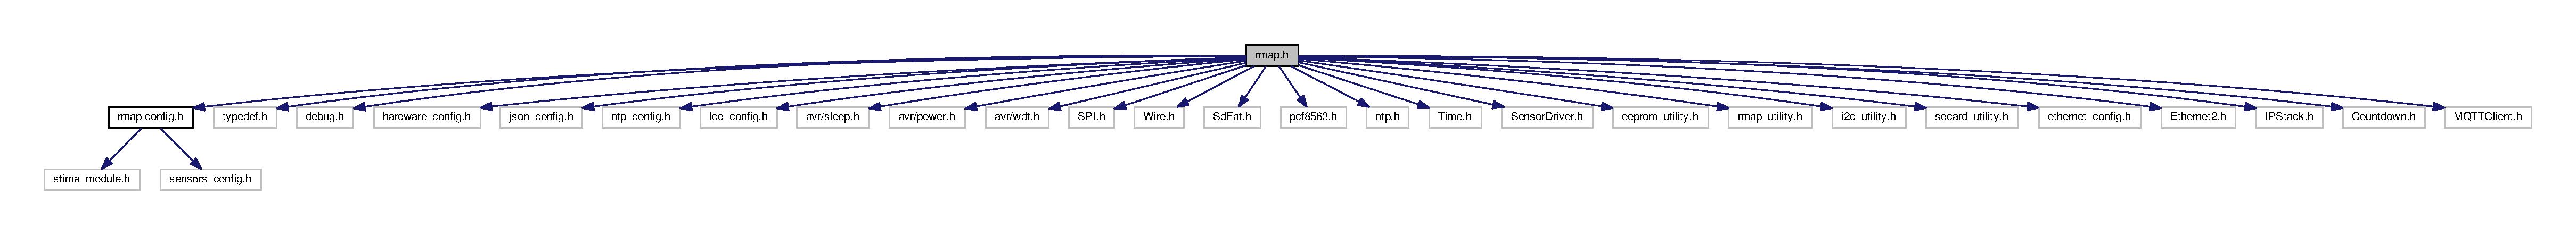
\includegraphics[width=350pt]{rmap_8h__incl}
\end{center}
\end{figure}
This graph shows which files directly or indirectly include this file\+:
\nopagebreak
\begin{figure}[H]
\begin{center}
\leavevmode
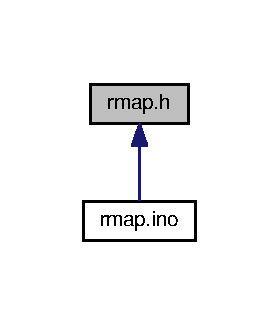
\includegraphics[width=196pt]{rmap_8h__dep__incl}
\end{center}
\end{figure}
\subsection*{Classes}
\begin{DoxyCompactItemize}
\item 
struct \hyperlink{structconfiguration__t}{configuration\+\_\+t}
\begin{DoxyCompactList}\small\item\em E\+E\+P\+R\+OM saved configuration. \end{DoxyCompactList}\end{DoxyCompactItemize}
\subsection*{Enumerations}
\begin{DoxyCompactItemize}
\item 
enum \hyperlink{rmap_8h_aa0aafed44fec19806d8f9ad834be1248}{state\+\_\+t} \{ \newline
\hyperlink{i2c-rain_8h_aa0aafed44fec19806d8f9ad834be1248a0cb1b2c6a7db1f1084886c98909a3f36}{I\+N\+IT}, 
\hyperlink{i2c-rain_8h_aa0aafed44fec19806d8f9ad834be1248a34f1df650a5075369a6827770c433a91}{T\+A\+S\+K\+S\+\_\+\+E\+X\+E\+C\+U\+T\+I\+ON}, 
\hyperlink{i2c-rain_8h_aa0aafed44fec19806d8f9ad834be1248adc6f24fd6915a3f2786a1b7045406924}{E\+ND}, 
\hyperlink{i2c-th_8h_aa0aafed44fec19806d8f9ad834be1248a0cb1b2c6a7db1f1084886c98909a3f36}{I\+N\+IT}, 
\newline
\hyperlink{i2c-th_8h_aa0aafed44fec19806d8f9ad834be1248a34f1df650a5075369a6827770c433a91}{T\+A\+S\+K\+S\+\_\+\+E\+X\+E\+C\+U\+T\+I\+ON}, 
\hyperlink{i2c-th_8h_aa0aafed44fec19806d8f9ad834be1248adc6f24fd6915a3f2786a1b7045406924}{E\+ND}, 
\hyperlink{rmap_8h_aa0aafed44fec19806d8f9ad834be1248a0cb1b2c6a7db1f1084886c98909a3f36}{I\+N\+IT}, 
\hyperlink{rmap_8h_aa0aafed44fec19806d8f9ad834be1248a34f1df650a5075369a6827770c433a91}{T\+A\+S\+K\+S\+\_\+\+E\+X\+E\+C\+U\+T\+I\+ON}, 
\newline
\hyperlink{rmap_8h_aa0aafed44fec19806d8f9ad834be1248adc6f24fd6915a3f2786a1b7045406924}{E\+ND}
 \}
\item 
enum \hyperlink{rmap_8h_a3a75eeb98a0ff1f3689694fa76711296}{supervisor\+\_\+state\+\_\+t} \{ \newline
\hyperlink{rmap_8h_a3a75eeb98a0ff1f3689694fa76711296a363ccb4e9e123cf22fb0e3b280964961}{S\+U\+P\+E\+R\+V\+I\+S\+O\+R\+\_\+\+I\+N\+IT}, 
\hyperlink{rmap_8h_a3a75eeb98a0ff1f3689694fa76711296ae7005d420b6eebd40ad507ac8b7dbc19}{S\+U\+P\+E\+R\+V\+I\+S\+O\+R\+\_\+\+C\+O\+N\+N\+E\+C\+T\+I\+O\+N\+\_\+\+L\+E\+V\+E\+L\+\_\+\+T\+A\+SK}, 
\hyperlink{rmap_8h_a3a75eeb98a0ff1f3689694fa76711296a8a66e5b3f27cba640fc2361ec510a610}{S\+U\+P\+E\+R\+V\+I\+S\+O\+R\+\_\+\+W\+A\+I\+T\+\_\+\+C\+O\+N\+N\+E\+C\+T\+I\+O\+N\+\_\+\+L\+E\+V\+E\+L\+\_\+\+T\+A\+SK}, 
\hyperlink{rmap_8h_a3a75eeb98a0ff1f3689694fa76711296a4808544db525d23b15d75770b1c770dd}{S\+U\+P\+E\+R\+V\+I\+S\+O\+R\+\_\+\+T\+I\+M\+E\+\_\+\+L\+E\+V\+E\+L\+\_\+\+T\+A\+SK}, 
\newline
\hyperlink{rmap_8h_a3a75eeb98a0ff1f3689694fa76711296aa832a47126ddf8bf542fd467854200a1}{S\+U\+P\+E\+R\+V\+I\+S\+O\+R\+\_\+\+M\+A\+N\+A\+G\+E\+\_\+\+L\+E\+V\+E\+L\+\_\+\+T\+A\+SK}, 
\hyperlink{rmap_8h_a3a75eeb98a0ff1f3689694fa76711296ac6b695b8e38a80dc56aa57beec7a0279}{S\+U\+P\+E\+R\+V\+I\+S\+O\+R\+\_\+\+E\+ND}, 
\hyperlink{rmap_8h_a3a75eeb98a0ff1f3689694fa76711296a42cba049478891fe2685e6aa11695838}{S\+U\+P\+E\+R\+V\+I\+S\+O\+R\+\_\+\+W\+A\+I\+T\+\_\+\+S\+T\+A\+TE}
 \}\begin{DoxyCompactList}\small\item\em Supervisor task finite state machine. \end{DoxyCompactList}
\item 
enum \hyperlink{rmap_8h_a41694caa7c2afa9fa0f9b3eae96246e5}{ethernet\+\_\+state\+\_\+t} \{ \newline
\hyperlink{rmap_8h_a41694caa7c2afa9fa0f9b3eae96246e5ae749f72358acfad64bb00e3461f4cbc2}{E\+T\+H\+E\+R\+N\+E\+T\+\_\+\+I\+N\+IT}, 
\hyperlink{rmap_8h_a41694caa7c2afa9fa0f9b3eae96246e5a95426b8bbfdb86442c9e41a139f8ae3c}{E\+T\+H\+E\+R\+N\+E\+T\+\_\+\+C\+O\+N\+N\+E\+CT}, 
\hyperlink{rmap_8h_a41694caa7c2afa9fa0f9b3eae96246e5aa12a74aa444cd4e24b43d3e280fc5044}{E\+T\+H\+E\+R\+N\+E\+T\+\_\+\+O\+P\+E\+N\+\_\+\+U\+D\+P\+\_\+\+S\+O\+C\+K\+ET}, 
\hyperlink{rmap_8h_a41694caa7c2afa9fa0f9b3eae96246e5a8869bbdcd969ee43efef6b882780bc5b}{E\+T\+H\+E\+R\+N\+E\+T\+\_\+\+E\+ND}, 
\newline
\hyperlink{rmap_8h_a41694caa7c2afa9fa0f9b3eae96246e5ada078050168a00fc4e3b5b4c345aa7bc}{E\+T\+H\+E\+R\+N\+E\+T\+\_\+\+W\+A\+I\+T\+\_\+\+S\+T\+A\+TE}
 \}\begin{DoxyCompactList}\small\item\em Ethernet task finite state machine. \end{DoxyCompactList}
\item 
enum \hyperlink{rmap_8h_a48bef3d022ff6f88967496ad53a6b953}{sensors\+\_\+reading\+\_\+state\+\_\+t} \{ \newline
\hyperlink{i2c-th_8h_a48bef3d022ff6f88967496ad53a6b953a2cb28b4d2ce509fc382d6bd1b2d5d16f}{S\+E\+N\+S\+O\+R\+S\+\_\+\+R\+E\+A\+D\+I\+N\+G\+\_\+\+I\+N\+IT}, 
\hyperlink{i2c-th_8h_a48bef3d022ff6f88967496ad53a6b953a7cf0f5ecc300e86aacc2deb266d14724}{S\+E\+N\+S\+O\+R\+S\+\_\+\+R\+E\+A\+D\+I\+N\+G\+\_\+\+P\+R\+E\+P\+A\+RE}, 
\hyperlink{i2c-th_8h_a48bef3d022ff6f88967496ad53a6b953a96e335eefffa76f53459df4a3cf71ac1}{S\+E\+N\+S\+O\+R\+S\+\_\+\+R\+E\+A\+D\+I\+N\+G\+\_\+\+I\+S\+\_\+\+P\+R\+E\+P\+A\+R\+ED}, 
\hyperlink{i2c-th_8h_a48bef3d022ff6f88967496ad53a6b953a8e031386ec7bcc225e75a4a0b408d731}{S\+E\+N\+S\+O\+R\+S\+\_\+\+R\+E\+A\+D\+I\+N\+G\+\_\+\+G\+ET}, 
\newline
\hyperlink{i2c-th_8h_a48bef3d022ff6f88967496ad53a6b953a3dae8abf31ae3db2ab2d679c224fd8be}{S\+E\+N\+S\+O\+R\+S\+\_\+\+R\+E\+A\+D\+I\+N\+G\+\_\+\+I\+S\+\_\+\+G\+E\+T\+T\+ED}, 
\hyperlink{i2c-th_8h_a48bef3d022ff6f88967496ad53a6b953ac2ebb8ebf9d29905d0a30f804376b9fa}{S\+E\+N\+S\+O\+R\+S\+\_\+\+R\+E\+A\+D\+I\+N\+G\+\_\+\+R\+E\+AD}, 
\hyperlink{i2c-th_8h_a48bef3d022ff6f88967496ad53a6b953a739c69b8d018187b0956660ed209e303}{S\+E\+N\+S\+O\+R\+S\+\_\+\+R\+E\+A\+D\+I\+N\+G\+\_\+\+N\+E\+XT}, 
\hyperlink{i2c-th_8h_a48bef3d022ff6f88967496ad53a6b953ab602220e588f3c2ac15b450239d9577a}{S\+E\+N\+S\+O\+R\+S\+\_\+\+R\+E\+A\+D\+I\+N\+G\+\_\+\+E\+ND}, 
\newline
\hyperlink{i2c-th_8h_a48bef3d022ff6f88967496ad53a6b953acfc850b971651f7c8c90cddf593fa399}{S\+E\+N\+S\+O\+R\+S\+\_\+\+R\+E\+A\+D\+I\+N\+G\+\_\+\+W\+A\+I\+T\+\_\+\+S\+T\+A\+TE}, 
\hyperlink{rmap_8h_a48bef3d022ff6f88967496ad53a6b953a2cb28b4d2ce509fc382d6bd1b2d5d16f}{S\+E\+N\+S\+O\+R\+S\+\_\+\+R\+E\+A\+D\+I\+N\+G\+\_\+\+I\+N\+IT}, 
\hyperlink{rmap_8h_a48bef3d022ff6f88967496ad53a6b953a7cf0f5ecc300e86aacc2deb266d14724}{S\+E\+N\+S\+O\+R\+S\+\_\+\+R\+E\+A\+D\+I\+N\+G\+\_\+\+P\+R\+E\+P\+A\+RE}, 
\hyperlink{rmap_8h_a48bef3d022ff6f88967496ad53a6b953a96e335eefffa76f53459df4a3cf71ac1}{S\+E\+N\+S\+O\+R\+S\+\_\+\+R\+E\+A\+D\+I\+N\+G\+\_\+\+I\+S\+\_\+\+P\+R\+E\+P\+A\+R\+ED}, 
\newline
\hyperlink{rmap_8h_a48bef3d022ff6f88967496ad53a6b953a8e031386ec7bcc225e75a4a0b408d731}{S\+E\+N\+S\+O\+R\+S\+\_\+\+R\+E\+A\+D\+I\+N\+G\+\_\+\+G\+ET}, 
\hyperlink{rmap_8h_a48bef3d022ff6f88967496ad53a6b953a3dae8abf31ae3db2ab2d679c224fd8be}{S\+E\+N\+S\+O\+R\+S\+\_\+\+R\+E\+A\+D\+I\+N\+G\+\_\+\+I\+S\+\_\+\+G\+E\+T\+T\+ED}, 
\hyperlink{rmap_8h_a48bef3d022ff6f88967496ad53a6b953ac2ebb8ebf9d29905d0a30f804376b9fa}{S\+E\+N\+S\+O\+R\+S\+\_\+\+R\+E\+A\+D\+I\+N\+G\+\_\+\+R\+E\+AD}, 
\hyperlink{rmap_8h_a48bef3d022ff6f88967496ad53a6b953a739c69b8d018187b0956660ed209e303}{S\+E\+N\+S\+O\+R\+S\+\_\+\+R\+E\+A\+D\+I\+N\+G\+\_\+\+N\+E\+XT}, 
\newline
\hyperlink{rmap_8h_a48bef3d022ff6f88967496ad53a6b953ab602220e588f3c2ac15b450239d9577a}{S\+E\+N\+S\+O\+R\+S\+\_\+\+R\+E\+A\+D\+I\+N\+G\+\_\+\+E\+ND}, 
\hyperlink{rmap_8h_a48bef3d022ff6f88967496ad53a6b953acfc850b971651f7c8c90cddf593fa399}{S\+E\+N\+S\+O\+R\+S\+\_\+\+R\+E\+A\+D\+I\+N\+G\+\_\+\+W\+A\+I\+T\+\_\+\+S\+T\+A\+TE}
 \}
\item 
enum \hyperlink{rmap_8h_a70deb66f62f31f2e15c734513dc0092a}{time\+\_\+state\+\_\+t} \{ \newline
\hyperlink{rmap_8h_a70deb66f62f31f2e15c734513dc0092aa74247eca9c928de916c1d25055cfce4c}{T\+I\+M\+E\+\_\+\+I\+N\+IT}, 
\hyperlink{rmap_8h_a70deb66f62f31f2e15c734513dc0092aab9e041a5c5be51544fe8a923da7a534b}{T\+I\+M\+E\+\_\+\+S\+E\+N\+D\+\_\+\+O\+N\+L\+I\+N\+E\+\_\+\+R\+E\+Q\+U\+E\+ST}, 
\hyperlink{rmap_8h_a70deb66f62f31f2e15c734513dc0092aa36b665f47ddd47fe4ff903d2cdec77c4}{T\+I\+M\+E\+\_\+\+W\+A\+I\+T\+\_\+\+O\+N\+L\+I\+N\+E\+\_\+\+R\+E\+S\+P\+O\+N\+SE}, 
\hyperlink{rmap_8h_a70deb66f62f31f2e15c734513dc0092aada3c6a7b36ab0c2fbdb62e99e576fd87}{T\+I\+M\+E\+\_\+\+S\+E\+T\+\_\+\+S\+Y\+N\+C\+\_\+\+N\+T\+P\+\_\+\+P\+R\+O\+V\+I\+D\+ER}, 
\newline
\hyperlink{rmap_8h_a70deb66f62f31f2e15c734513dc0092aa69c34bd14a9fc8eeb55a37163f7774a4}{T\+I\+M\+E\+\_\+\+S\+E\+T\+\_\+\+S\+Y\+N\+C\+\_\+\+R\+T\+C\+\_\+\+P\+R\+O\+V\+I\+D\+ER}, 
\hyperlink{rmap_8h_a70deb66f62f31f2e15c734513dc0092aa43fcb32d8eb7b4b3ae69a20356ae484b}{T\+I\+M\+E\+\_\+\+E\+ND}, 
\hyperlink{rmap_8h_a70deb66f62f31f2e15c734513dc0092aa834d29edc9046ba5706bc4b17bcbb447}{T\+I\+M\+E\+\_\+\+W\+A\+I\+T\+\_\+\+S\+T\+A\+TE}
 \}\begin{DoxyCompactList}\small\item\em Time task finite state machine. \end{DoxyCompactList}
\item 
enum \hyperlink{rmap_8h_a890f00ea5c43b52d0acd0d2dbc67e188}{data\+\_\+saving\+\_\+state\+\_\+t} \{ \newline
\hyperlink{rmap_8h_a890f00ea5c43b52d0acd0d2dbc67e188a9676cb6137dc982a78008b74d04c4129}{D\+A\+T\+A\+\_\+\+S\+A\+V\+I\+N\+G\+\_\+\+I\+N\+IT}, 
\hyperlink{rmap_8h_a890f00ea5c43b52d0acd0d2dbc67e188ae39f03e395bf182e7f92cc16b98fc2de}{D\+A\+T\+A\+\_\+\+S\+A\+V\+I\+N\+G\+\_\+\+O\+P\+E\+N\+\_\+\+S\+D\+C\+A\+RD}, 
\hyperlink{rmap_8h_a890f00ea5c43b52d0acd0d2dbc67e188aac704d8a92ae0c74182d5c208969abe3}{D\+A\+T\+A\+\_\+\+S\+A\+V\+I\+N\+G\+\_\+\+O\+P\+E\+N\+\_\+\+F\+I\+LE}, 
\hyperlink{rmap_8h_a890f00ea5c43b52d0acd0d2dbc67e188ae6689e6f9a0f334a0bd0ab41dae53fd7}{D\+A\+T\+A\+\_\+\+S\+A\+V\+I\+N\+G\+\_\+\+S\+E\+N\+S\+O\+R\+S\+\_\+\+L\+O\+OP}, 
\newline
\hyperlink{rmap_8h_a890f00ea5c43b52d0acd0d2dbc67e188aaf8488faff968be1f0fdfaedefea746b}{D\+A\+T\+A\+\_\+\+S\+A\+V\+I\+N\+G\+\_\+\+D\+A\+T\+A\+\_\+\+L\+O\+OP}, 
\hyperlink{rmap_8h_a890f00ea5c43b52d0acd0d2dbc67e188afd990e9f452cde112bd60e50df97be33}{D\+A\+T\+A\+\_\+\+S\+A\+V\+I\+N\+G\+\_\+\+W\+R\+I\+T\+E\+\_\+\+F\+I\+LE}, 
\hyperlink{rmap_8h_a890f00ea5c43b52d0acd0d2dbc67e188a97fa8a54ea5583f9c4b2e58040f57dfd}{D\+A\+T\+A\+\_\+\+S\+A\+V\+I\+N\+G\+\_\+\+C\+L\+O\+S\+E\+\_\+\+F\+I\+LE}, 
\hyperlink{rmap_8h_a890f00ea5c43b52d0acd0d2dbc67e188ac860ad4ac8467961fc82620e5cfb7c5b}{D\+A\+T\+A\+\_\+\+S\+A\+V\+I\+N\+G\+\_\+\+E\+ND}, 
\newline
\hyperlink{rmap_8h_a890f00ea5c43b52d0acd0d2dbc67e188ac5e868c6debf468cb0d0831df2c616ef}{D\+A\+T\+A\+\_\+\+S\+A\+V\+I\+N\+G\+\_\+\+W\+A\+I\+T\+\_\+\+S\+T\+A\+TE}
 \}\begin{DoxyCompactList}\small\item\em Data saving task finite state machine. \end{DoxyCompactList}
\item 
enum \hyperlink{rmap_8h_a9eecd1044ddb5510b71716eedfd15f2a}{mqtt\+\_\+state\+\_\+t} \{ \newline
\hyperlink{rmap_8h_a9eecd1044ddb5510b71716eedfd15f2aab78e0d91fcdd4c3b9fa2a8daf8da61ee}{M\+Q\+T\+T\+\_\+\+I\+N\+IT}, 
\hyperlink{rmap_8h_a9eecd1044ddb5510b71716eedfd15f2aa6f072da1e81e5ddb573f53214aef5c29}{M\+Q\+T\+T\+\_\+\+O\+P\+E\+N\+\_\+\+S\+D\+C\+A\+RD}, 
\hyperlink{rmap_8h_a9eecd1044ddb5510b71716eedfd15f2aa333fe1685d303726beaf4ab7f79675dc}{M\+Q\+T\+T\+\_\+\+O\+P\+E\+N\+\_\+\+P\+T\+R\+\_\+\+F\+I\+LE}, 
\hyperlink{rmap_8h_a9eecd1044ddb5510b71716eedfd15f2aa88ef6d59236afb176577d29232ac2dbe}{M\+Q\+T\+T\+\_\+\+P\+T\+R\+\_\+\+R\+E\+AD}, 
\newline
\hyperlink{rmap_8h_a9eecd1044ddb5510b71716eedfd15f2aa4c14dda1eb0b6815720a8825c51a972f}{M\+Q\+T\+T\+\_\+\+P\+T\+R\+\_\+\+F\+I\+ND}, 
\hyperlink{rmap_8h_a9eecd1044ddb5510b71716eedfd15f2aafb016951f241118473fa441f9e255716}{M\+Q\+T\+T\+\_\+\+P\+T\+R\+\_\+\+F\+O\+U\+ND}, 
\hyperlink{rmap_8h_a9eecd1044ddb5510b71716eedfd15f2aa976c127fbaa0c71ff67c039a6ead4270}{M\+Q\+T\+T\+\_\+\+P\+T\+R\+\_\+\+E\+ND}, 
\hyperlink{rmap_8h_a9eecd1044ddb5510b71716eedfd15f2aafc9e8686794d1ce791b2d50be3e0b718}{M\+Q\+T\+T\+\_\+\+O\+P\+EN}, 
\newline
\hyperlink{rmap_8h_a9eecd1044ddb5510b71716eedfd15f2aab8bd5fe2df05cf458706f4746031101f}{M\+Q\+T\+T\+\_\+\+C\+H\+E\+CK}, 
\hyperlink{rmap_8h_a9eecd1044ddb5510b71716eedfd15f2aa1f01f8e725b363e6b107d3d8cfc8586b}{M\+Q\+T\+T\+\_\+\+C\+O\+N\+N\+E\+CT}, 
\hyperlink{rmap_8h_a9eecd1044ddb5510b71716eedfd15f2aa5d00f1aedfa96cebd92f9ee837c3a615}{M\+Q\+T\+T\+\_\+\+O\+N\+\_\+\+C\+O\+N\+N\+E\+CT}, 
\hyperlink{rmap_8h_a9eecd1044ddb5510b71716eedfd15f2aa7dd20d5d68728190c8c1050599b562f7}{M\+Q\+T\+T\+\_\+\+S\+U\+B\+S\+C\+R\+I\+BE}, 
\newline
\hyperlink{rmap_8h_a9eecd1044ddb5510b71716eedfd15f2aa559395ca103488b50d5cb1bebd24a539}{M\+Q\+T\+T\+\_\+\+O\+P\+E\+N\+\_\+\+D\+A\+T\+A\+\_\+\+F\+I\+LE}, 
\hyperlink{rmap_8h_a9eecd1044ddb5510b71716eedfd15f2aab8529974dafdcc57ae96953df84c4d23}{M\+Q\+T\+T\+\_\+\+S\+E\+N\+S\+O\+R\+S\+\_\+\+L\+O\+OP}, 
\hyperlink{rmap_8h_a9eecd1044ddb5510b71716eedfd15f2aabfd381e8944cbb38db3ae9e26be8e5fa}{M\+Q\+T\+T\+\_\+\+D\+A\+T\+A\+\_\+\+L\+O\+OP}, 
\hyperlink{rmap_8h_a9eecd1044ddb5510b71716eedfd15f2aaa374bf000fce299ee44a155c315be872}{M\+Q\+T\+T\+\_\+\+S\+D\+\_\+\+L\+O\+OP}, 
\newline
\hyperlink{rmap_8h_a9eecd1044ddb5510b71716eedfd15f2aa18f5c91ee58e3c7af217a99d06bce38a}{M\+Q\+T\+T\+\_\+\+P\+U\+B\+L\+I\+SH}, 
\hyperlink{rmap_8h_a9eecd1044ddb5510b71716eedfd15f2aadd96b9c4ec8178e82fbbaea103f0af4c}{M\+Q\+T\+T\+\_\+\+C\+L\+O\+S\+E\+\_\+\+D\+A\+T\+A\+\_\+\+F\+I\+LE}, 
\hyperlink{rmap_8h_a9eecd1044ddb5510b71716eedfd15f2aa247d31e0fa0c828dfc7e7d2d22ca18b2}{M\+Q\+T\+T\+\_\+\+D\+I\+S\+C\+O\+N\+N\+E\+CT}, 
\hyperlink{rmap_8h_a9eecd1044ddb5510b71716eedfd15f2aaf72d33e5f5a66855c0f30a1b1184d948}{M\+Q\+T\+T\+\_\+\+O\+N\+\_\+\+D\+I\+S\+C\+O\+N\+N\+E\+CT}, 
\newline
\hyperlink{rmap_8h_a9eecd1044ddb5510b71716eedfd15f2aa373d63f35bc88e697f24d68c1685a0b2}{M\+Q\+T\+T\+\_\+\+P\+T\+R\+\_\+\+U\+P\+D\+A\+TE}, 
\hyperlink{rmap_8h_a9eecd1044ddb5510b71716eedfd15f2aa87cbbb025c198e8a13e05e43090b1012}{M\+Q\+T\+T\+\_\+\+C\+L\+O\+S\+E\+\_\+\+P\+T\+R\+\_\+\+F\+I\+LE}, 
\hyperlink{rmap_8h_a9eecd1044ddb5510b71716eedfd15f2aa45ee7f65a13484d4aa294bc91c0bc452}{M\+Q\+T\+T\+\_\+\+C\+L\+O\+S\+E\+\_\+\+S\+D\+C\+A\+RD}, 
\hyperlink{rmap_8h_a9eecd1044ddb5510b71716eedfd15f2aa1c2b0cefef6f30ebcfa09ac728a41aa5}{M\+Q\+T\+T\+\_\+\+E\+ND}, 
\newline
\hyperlink{rmap_8h_a9eecd1044ddb5510b71716eedfd15f2aa690eaf72810b51357bbf8ae62e62cfb6}{M\+Q\+T\+T\+\_\+\+W\+A\+I\+T\+\_\+\+S\+T\+A\+TE}
 \}\begin{DoxyCompactList}\small\item\em M\+Q\+TT task finite state machine. \end{DoxyCompactList}
\item 
enum \hyperlink{rmap_8h_a94235530fc35d5e307de374cfca8b7ab}{stream\+\_\+state\+\_\+t} \{ \hyperlink{rmap_8h_a94235530fc35d5e307de374cfca8b7aba541f21a61fd4ffca270456e725781f7a}{S\+T\+R\+E\+A\+M\+\_\+\+I\+N\+IT}, 
\hyperlink{rmap_8h_a94235530fc35d5e307de374cfca8b7abab5d8bf74432bd63537b006e770df3fed}{S\+T\+R\+E\+A\+M\+\_\+\+A\+V\+A\+I\+L\+A\+B\+LE}, 
\hyperlink{rmap_8h_a94235530fc35d5e307de374cfca8b7abab9b72ed53e734c811d2de663ac42d0cd}{S\+T\+R\+E\+A\+M\+\_\+\+P\+R\+O\+C\+E\+SS}, 
\hyperlink{rmap_8h_a94235530fc35d5e307de374cfca8b7aba53fa1bd490c433482f76aa289f43b487}{S\+T\+R\+E\+A\+M\+\_\+\+E\+ND}
 \}\begin{DoxyCompactList}\small\item\em Stream task finite state machine. \end{DoxyCompactList}
\end{DoxyCompactItemize}
\subsection*{Functions}
\begin{DoxyCompactItemize}
\item 
I\+P\+Stack \hyperlink{rmap_8h_a447e41b96c37bcba88cba66f6ebb7878}{ipstack} (\hyperlink{rmap_8h_abdcb198b5489995a350bc73d1d5f4f6d}{eth\+\_\+tcp\+\_\+client})
\begin{DoxyCompactList}\small\item\em Ethernet I\+P\+Stack M\+Q\+T\+T\+Client structure. \end{DoxyCompactList}\item 
Liquid\+Crystal\+\_\+\+I2C \hyperlink{rmap_8h_af7d08a33a932b4784cae528e8219f1c7}{lcd} (\hyperlink{lcd__config_8h_aabe3eae58b7e15bab0e4e34245079410}{L\+C\+D\+\_\+\+I2\+C\+\_\+\+A\+D\+D\+R\+E\+SS}, \hyperlink{lcd__config_8h_a537e0d54d9ec6c708bd8990c2f4d8e64}{L\+C\+D\+\_\+\+C\+O\+L\+U\+M\+NS}, \hyperlink{lcd__config_8h_a9a59fc4d524d3519a6bd0cb451850a65}{L\+C\+D\+\_\+\+R\+O\+WS})
\begin{DoxyCompactList}\small\item\em L\+CD structure. \end{DoxyCompactList}\item 
void \hyperlink{rmap_8h_afb98a0f07c30784284f48271ffe02b97}{init\+\_\+power\+\_\+down} (uint32\+\_\+t $\ast$time\+\_\+ms, uint32\+\_\+t debouncing\+\_\+ms)
\begin{DoxyCompactList}\small\item\em Enter power down mode. \end{DoxyCompactList}\item 
void \hyperlink{rmap_8h_a980e73df66b14b1190bc25da430a4f12}{init\+\_\+wdt} (uint8\+\_\+t wdt\+\_\+timer)
\begin{DoxyCompactList}\small\item\em Init watchdog. \end{DoxyCompactList}\item 
void \hyperlink{rmap_8h_a348d23d5899ce59d18975284dfb0afc0}{init\+\_\+system} (void)
\begin{DoxyCompactList}\small\item\em Init system. \end{DoxyCompactList}\item 
void \hyperlink{rmap_8h_ad438327c9cf783bd9c519ce8b8ef3bfa}{init\+\_\+buffers} (void)
\begin{DoxyCompactList}\small\item\em Init buffers. \end{DoxyCompactList}\item 
void \hyperlink{rmap_8h_a2aae2290a141fddcea3fb6009acbb445}{init\+\_\+tasks} (void)
\begin{DoxyCompactList}\small\item\em Init tasks variable and state. \end{DoxyCompactList}\item 
void \hyperlink{rmap_8h_aa9c113540346b54d49b2a596e6ba8480}{init\+\_\+pins} (void)
\begin{DoxyCompactList}\small\item\em Init hardware pins. \end{DoxyCompactList}\item 
void \hyperlink{rmap_8h_a7c21452937863fa02a29654247eef09b}{init\+\_\+wire} (void)
\begin{DoxyCompactList}\small\item\em Init wire (i2c) library and performs checks on the bus. \end{DoxyCompactList}\item 
void \hyperlink{rmap_8h_a4454f968b2402a0e61deb15ab2571dab}{init\+\_\+spi} (void)
\begin{DoxyCompactList}\small\item\em Init S\+PI library. \end{DoxyCompactList}\item 
void \hyperlink{rmap_8h_a88533ad02465ce52d4e6de7b2095ec32}{init\+\_\+rtc} (void)
\begin{DoxyCompactList}\small\item\em Init R\+TC module. \end{DoxyCompactList}\item 
void \hyperlink{rmap_8h_ad7577ba7f06f417a019b69da8682ede5}{init\+\_\+sensors} (void)
\begin{DoxyCompactList}\small\item\em Create and setup sensors. \end{DoxyCompactList}\item 
void \hyperlink{rmap_8h_ab08b9047f47849f399950705e769be2e}{print\+\_\+configuration} (void)
\begin{DoxyCompactList}\small\item\em Print current configuration. \end{DoxyCompactList}\item 
void \hyperlink{rmap_8h_a1be652e7d942160a14a560e0be837358}{load\+\_\+configuration} (void)
\begin{DoxyCompactList}\small\item\em Load configuration from E\+E\+P\+R\+OM. \end{DoxyCompactList}\item 
void \hyperlink{rmap_8h_a8801fa7c9f323c5b8b9b2bb5b1c438ff}{save\+\_\+configuration} (bool)
\begin{DoxyCompactList}\small\item\em Save configuration to E\+E\+P\+R\+OM. \end{DoxyCompactList}\item 
void \hyperlink{rmap_8h_a90fe8c7d55bc889ad3ede7c76207e6a8}{set\+\_\+default\+\_\+configuration} (void)
\begin{DoxyCompactList}\small\item\em Set default configuration to global configuration variable. \end{DoxyCompactList}\item 
void \hyperlink{rmap_8h_a1686e2719fa4a37ef933458673973d28}{set\+Next\+Time\+For\+Sensor\+Reading} (time\+\_\+t $\ast$next\+\_\+time)
\begin{DoxyCompactList}\small\item\em Calculate next hour, minute and second for sensors reading. \end{DoxyCompactList}\item 
bool \hyperlink{rmap_8h_a9f5e5ca8c47d4536dd1805e89fbb7db2}{mqtt\+Connect} (char $\ast$username, char $\ast$password)
\begin{DoxyCompactList}\small\item\em Use a open tcp socket to connect to the mqtt server. \end{DoxyCompactList}\item 
bool \hyperlink{rmap_8h_aa0d50218413a12917f8c70ef4e1e1e72}{mqtt\+Publish} (const char $\ast$topic, const char $\ast$message)
\begin{DoxyCompactList}\small\item\em Publish message on topic. \end{DoxyCompactList}\item 
void \hyperlink{rmap_8h_a4fe2f970295d296f7f6725fe9e946933}{mqtt\+Rx\+Callback} (M\+Q\+T\+T\+::\+Message\+Data \&md)
\begin{DoxyCompactList}\small\item\em Register a receive callback for incoming mqtt message. \end{DoxyCompactList}\item 
char $\ast$ \hyperlink{rmap_8h_afba6e70a8bee4b42785eaeca4fd566d3}{rpc\+\_\+process} (char $\ast$json)
\begin{DoxyCompactList}\small\item\em Process and execute a received Remote Procedure Call (R\+PC). Useful for configuration. \end{DoxyCompactList}\item 
void \hyperlink{rmap_8h_a1c0ac3dbd03144160dd35a3c8674d9b3}{supervisor\+\_\+task} (void)
\begin{DoxyCompactList}\small\item\em Supervisor task. Manage R\+TC and N\+TP sync and open/close gsm and ethernet connection. \end{DoxyCompactList}\item 
void \hyperlink{rmap_8h_af0e8965583b124096972fe3a9e0e7954}{sensors\+\_\+reading\+\_\+task} (void)
\begin{DoxyCompactList}\small\item\em Sensors reading Task. Read data from sensors. \end{DoxyCompactList}\item 
void \hyperlink{rmap_8h_a5099cc10afd8a26fdd8599574f0fc5a8}{rtc\+\_\+task} (void)
\begin{DoxyCompactList}\small\item\em Real Time Clock task. Read R\+TC time and sync system time with it. \end{DoxyCompactList}\item 
void \hyperlink{rmap_8h_a5069fdc64788136358f93a124624d05d}{time\+\_\+task} (void)
\begin{DoxyCompactList}\small\item\em Time task. Get time from N\+TP and sync R\+TC with it. \end{DoxyCompactList}\item 
void \hyperlink{rmap_8h_ab468f998bb8b3e07fe2b4325d359a8ec}{ethernet\+\_\+task} (void)
\begin{DoxyCompactList}\small\item\em Ethernet task. Manage Ethernet operation. \end{DoxyCompactList}\item 
void \hyperlink{rmap_8h_ae49b822b37337a0744225c3bdd43c79c}{data\+\_\+saving\+\_\+task} (void)
\begin{DoxyCompactList}\small\item\em Data Saving Task. Save acquired sensors data on S\+D-\/\+Card. \end{DoxyCompactList}\item 
void \hyperlink{rmap_8h_ad0a96c657cfe5d9ec637fbe1731a7bd6}{mqtt\+\_\+task} (void)
\begin{DoxyCompactList}\small\item\em M\+Q\+TT Task. \end{DoxyCompactList}\item 
bool \hyperlink{rmap_8h_a21575354e8ec54fa31f581ed1838be79}{stream\+\_\+task} (Stream $\ast$stream, uint32\+\_\+t stream\+\_\+timeout, uint32\+\_\+t end\+\_\+task\+\_\+timeout)
\begin{DoxyCompactList}\small\item\em Stream Task. \end{DoxyCompactList}\item 
void \hyperlink{rmap_8h_ad61a7a94cdd76d63031bbe2972057659}{rtc\+\_\+interrupt\+\_\+handler} (void)
\begin{DoxyCompactList}\small\item\em Real Time Clock interrupt handler. \end{DoxyCompactList}\end{DoxyCompactItemize}
\subsection*{Variables}
\begin{DoxyCompactItemize}
\item 
\mbox{\Hypertarget{rmap_8h_af0d633ce166aa2f6289c2170c5f8879a}\label{rmap_8h_af0d633ce166aa2f6289c2170c5f8879a}} 
\hyperlink{structconfiguration__t}{configuration\+\_\+t} \hyperlink{rmap_8h_af0d633ce166aa2f6289c2170c5f8879a}{readable\+\_\+configuration}
\begin{DoxyCompactList}\small\item\em Configuration for this module. \end{DoxyCompactList}\item 
\mbox{\Hypertarget{rmap_8h_a28f0b3b858571f1f06e37cece9d0bed7}\label{rmap_8h_a28f0b3b858571f1f06e37cece9d0bed7}} 
\hyperlink{structconfiguration__t}{configuration\+\_\+t} \hyperlink{rmap_8h_a28f0b3b858571f1f06e37cece9d0bed7}{writable\+\_\+configuration}
\begin{DoxyCompactList}\small\item\em Configuration for this module. \end{DoxyCompactList}\item 
\mbox{\Hypertarget{rmap_8h_ab51900c214aadb930a66e4581a5d205e}\label{rmap_8h_ab51900c214aadb930a66e4581a5d205e}} 
volatile uint8\+\_\+t {\bfseries ready\+\_\+tasks\+\_\+count}
\item 
\mbox{\Hypertarget{rmap_8h_a78178f418362740f92f9e8b16aebb380}\label{rmap_8h_a78178f418362740f92f9e8b16aebb380}} 
uint32\+\_\+t {\bfseries awakened\+\_\+event\+\_\+occurred\+\_\+time\+\_\+ms}
\item 
\mbox{\Hypertarget{rmap_8h_a552b54fa96e90cd6565fb71968e9fc5a}\label{rmap_8h_a552b54fa96e90cd6565fb71968e9fc5a}} 
Sd\+Fat \hyperlink{rmap_8h_a552b54fa96e90cd6565fb71968e9fc5a}{SD}
\begin{DoxyCompactList}\small\item\em S\+D-\/\+Card structure. \end{DoxyCompactList}\item 
\mbox{\Hypertarget{rmap_8h_accc3044dc5c2625353cfb41b309c883d}\label{rmap_8h_accc3044dc5c2625353cfb41b309c883d}} 
File \hyperlink{rmap_8h_accc3044dc5c2625353cfb41b309c883d}{read\+\_\+data\+\_\+file}
\begin{DoxyCompactList}\small\item\em File structure for read data stored on S\+D-\/\+Card. \end{DoxyCompactList}\item 
\mbox{\Hypertarget{rmap_8h_a5766a19f9e7176fe5573021ef49d6e5d}\label{rmap_8h_a5766a19f9e7176fe5573021ef49d6e5d}} 
File \hyperlink{rmap_8h_a5766a19f9e7176fe5573021ef49d6e5d}{write\+\_\+data\+\_\+file}
\begin{DoxyCompactList}\small\item\em File structure for write data stored on S\+D-\/\+Card. \end{DoxyCompactList}\item 
\mbox{\Hypertarget{rmap_8h_ad4b1a751f0188d2a28ab680482fc0984}\label{rmap_8h_ad4b1a751f0188d2a28ab680482fc0984}} 
File \hyperlink{rmap_8h_ad4b1a751f0188d2a28ab680482fc0984}{mqtt\+\_\+ptr\+\_\+file}
\begin{DoxyCompactList}\small\item\em File structure for read and write data pointer stored on S\+D-\/\+Card for mqtt send. \end{DoxyCompactList}\item 
\mbox{\Hypertarget{rmap_8h_a2765db5c6ff0cd5266f528c32d9e1377}\label{rmap_8h_a2765db5c6ff0cd5266f528c32d9e1377}} 
Ethernet\+U\+DP \hyperlink{rmap_8h_a2765db5c6ff0cd5266f528c32d9e1377}{eth\+\_\+udp\+\_\+client}
\begin{DoxyCompactList}\small\item\em Ethernet U\+DP client structure. \end{DoxyCompactList}\item 
\mbox{\Hypertarget{rmap_8h_abdcb198b5489995a350bc73d1d5f4f6d}\label{rmap_8h_abdcb198b5489995a350bc73d1d5f4f6d}} 
Ethernet\+Client \hyperlink{rmap_8h_abdcb198b5489995a350bc73d1d5f4f6d}{eth\+\_\+tcp\+\_\+client}
\begin{DoxyCompactList}\small\item\em Ethernet T\+CP client structure. \end{DoxyCompactList}\item 
\mbox{\Hypertarget{rmap_8h_a4ba5e40cce164049fd8104ea673e56a9}\label{rmap_8h_a4ba5e40cce164049fd8104ea673e56a9}} 
M\+Q\+T\+T\+::\+Client$<$ I\+P\+Stack, Countdown, \hyperlink{mqtt__config_8h_a6d3b5b0f9c41b605e608f7d460491be6}{M\+Q\+T\+T\+\_\+\+R\+O\+O\+T\+\_\+\+T\+O\+P\+I\+C\+\_\+\+L\+E\+N\+G\+TH}+\hyperlink{mqtt__config_8h_a85772fcdfe85fa51f02f3045c0aa7764}{M\+Q\+T\+T\+\_\+\+S\+E\+N\+S\+O\+R\+\_\+\+T\+O\+P\+I\+C\+\_\+\+L\+E\+N\+G\+TH}+\hyperlink{mqtt__config_8h_a0fff77926fd907aeb2c03f60600d136c}{M\+Q\+T\+T\+\_\+\+M\+E\+S\+S\+A\+G\+E\+\_\+\+L\+E\+N\+G\+TH}, 1 $>$ \hyperlink{rmap_8h_a4ba5e40cce164049fd8104ea673e56a9}{mqtt\+\_\+client} = M\+Q\+T\+T\+::\+Client$<$I\+P\+Stack, Countdown, \hyperlink{mqtt__config_8h_a6d3b5b0f9c41b605e608f7d460491be6}{M\+Q\+T\+T\+\_\+\+R\+O\+O\+T\+\_\+\+T\+O\+P\+I\+C\+\_\+\+L\+E\+N\+G\+TH}+\hyperlink{mqtt__config_8h_a85772fcdfe85fa51f02f3045c0aa7764}{M\+Q\+T\+T\+\_\+\+S\+E\+N\+S\+O\+R\+\_\+\+T\+O\+P\+I\+C\+\_\+\+L\+E\+N\+G\+TH}+\hyperlink{mqtt__config_8h_a0fff77926fd907aeb2c03f60600d136c}{M\+Q\+T\+T\+\_\+\+M\+E\+S\+S\+A\+G\+E\+\_\+\+L\+E\+N\+G\+TH}, 1$>$(\hyperlink{rmap_8h_a447e41b96c37bcba88cba66f6ebb7878}{ipstack}, \hyperlink{rmap-config_8h_a578ee6f26618a9f795fb5828663431f0}{I\+P\+\_\+\+S\+T\+A\+C\+K\+\_\+\+T\+I\+M\+E\+O\+U\+T\+\_\+\+MS})
\begin{DoxyCompactList}\small\item\em M\+Q\+TT Client structure. \end{DoxyCompactList}\item 
\mbox{\Hypertarget{rmap_8h_afe8658551453cd97976b7a1490deaf36}\label{rmap_8h_afe8658551453cd97976b7a1490deaf36}} 
\hyperlink{classSensorDriver}{Sensor\+Driver} $\ast$ {\bfseries sensors} \mbox{[}\hyperlink{rmap-config_8h_af18dc3de744722cb308451b7a705611b}{U\+S\+E\+\_\+\+S\+E\+N\+S\+O\+R\+S\+\_\+\+C\+O\+U\+NT}\mbox{]}
\item 
\mbox{\Hypertarget{rmap_8h_a2de58e7c37115b75e1c0dfe5f0c4a982}\label{rmap_8h_a2de58e7c37115b75e1c0dfe5f0c4a982}} 
bool \hyperlink{rmap_8h_a2de58e7c37115b75e1c0dfe5f0c4a982}{is\+\_\+first\+\_\+run}
\begin{DoxyCompactList}\small\item\em If true, the first reading of the sensors was performed. \end{DoxyCompactList}\item 
\mbox{\Hypertarget{rmap_8h_a07c4f36e092c5486b25f32b6f387d387}\label{rmap_8h_a07c4f36e092c5486b25f32b6f387d387}} 
bool \hyperlink{rmap_8h_a07c4f36e092c5486b25f32b6f387d387}{is\+\_\+time\+\_\+set}
\begin{DoxyCompactList}\small\item\em If true, the time was readed from rtc or ntp and was setted in system. \end{DoxyCompactList}\item 
\mbox{\Hypertarget{rmap_8h_a3b06b80d1e1827c8d1449af2bcf8a1d7}\label{rmap_8h_a3b06b80d1e1827c8d1449af2bcf8a1d7}} 
bool \hyperlink{rmap_8h_a3b06b80d1e1827c8d1449af2bcf8a1d7}{is\+\_\+time\+\_\+for\+\_\+sensors\+\_\+reading\+\_\+updated}
\begin{DoxyCompactList}\small\item\em If true, the next time has been calculated to read the sensors. \end{DoxyCompactList}\item 
\mbox{\Hypertarget{rmap_8h_af66035ffa50a0ca243f92d007f3dd3e5}\label{rmap_8h_af66035ffa50a0ca243f92d007f3dd3e5}} 
bool \hyperlink{rmap_8h_af66035ffa50a0ca243f92d007f3dd3e5}{is\+\_\+client\+\_\+connected}
\begin{DoxyCompactList}\small\item\em If true, the client (ethernet or gsm) was connected to socket (T\+CP or U\+DP). \end{DoxyCompactList}\item 
\mbox{\Hypertarget{rmap_8h_a58f6a93217bb39bd5aa74734db38af87}\label{rmap_8h_a58f6a93217bb39bd5aa74734db38af87}} 
bool \hyperlink{rmap_8h_a58f6a93217bb39bd5aa74734db38af87}{is\+\_\+client\+\_\+udp\+\_\+socket\+\_\+open}
\begin{DoxyCompactList}\small\item\em If true, the client (ethernet or gsm) was opened the U\+DP socket. \end{DoxyCompactList}\item 
\mbox{\Hypertarget{rmap_8h_abea8c8c20b73acadd6420f7f63d2990d}\label{rmap_8h_abea8c8c20b73acadd6420f7f63d2990d}} 
bool \hyperlink{rmap_8h_abea8c8c20b73acadd6420f7f63d2990d}{is\+\_\+event\+\_\+client\+\_\+executed}
\begin{DoxyCompactList}\small\item\em If true, the client has executed its task. \end{DoxyCompactList}\item 
\mbox{\Hypertarget{rmap_8h_ae116f3df71f37918212f970931571573}\label{rmap_8h_ae116f3df71f37918212f970931571573}} 
bool \hyperlink{rmap_8h_ae116f3df71f37918212f970931571573}{is\+\_\+event\+\_\+time\+\_\+executed}
\begin{DoxyCompactList}\small\item\em If true, the time task has executed. \end{DoxyCompactList}\item 
\mbox{\Hypertarget{rmap_8h_abd2d7990cd2b2e061711bfdc600cef38}\label{rmap_8h_abd2d7990cd2b2e061711bfdc600cef38}} 
bool \hyperlink{rmap_8h_abd2d7990cd2b2e061711bfdc600cef38}{do\+\_\+ntp\+\_\+sync}
\begin{DoxyCompactList}\small\item\em If true, you must update the time from ntp. \end{DoxyCompactList}\item 
\mbox{\Hypertarget{rmap_8h_ae43fef3f7a959fdfb3f657c4b7f71ad5}\label{rmap_8h_ae43fef3f7a959fdfb3f657c4b7f71ad5}} 
time\+\_\+t \hyperlink{rmap_8h_ae43fef3f7a959fdfb3f657c4b7f71ad5}{last\+\_\+ntp\+\_\+sync}
\begin{DoxyCompactList}\small\item\em Last date and time when ntp sync was performed. \end{DoxyCompactList}\item 
\mbox{\Hypertarget{rmap_8h_a14818043a8a96a96433b3af2a9f5821d}\label{rmap_8h_a14818043a8a96a96433b3af2a9f5821d}} 
time\+\_\+t \hyperlink{rmap_8h_a14818043a8a96a96433b3af2a9f5821d}{last\+\_\+lcd\+\_\+begin}
\begin{DoxyCompactList}\small\item\em Last date and time when L\+CD was initializated. \end{DoxyCompactList}\item 
\mbox{\Hypertarget{rmap_8h_ad5cfddd994a6ae87b425e5fad249627c}\label{rmap_8h_ad5cfddd994a6ae87b425e5fad249627c}} 
bool \hyperlink{rmap_8h_ad5cfddd994a6ae87b425e5fad249627c}{is\+\_\+sdcard\+\_\+open}
\begin{DoxyCompactList}\small\item\em If true, the S\+D-\/\+Card is ready. \end{DoxyCompactList}\item 
\mbox{\Hypertarget{rmap_8h_a01167fb785c25e02aa85971cd3661c83}\label{rmap_8h_a01167fb785c25e02aa85971cd3661c83}} 
bool \hyperlink{rmap_8h_a01167fb785c25e02aa85971cd3661c83}{is\+\_\+sdcard\+\_\+error}
\begin{DoxyCompactList}\small\item\em If true, the S\+D-\/\+Card is in error. \end{DoxyCompactList}\item 
\mbox{\Hypertarget{rmap_8h_ad357c442547dc2dffb84c3bb00ca598f}\label{rmap_8h_ad357c442547dc2dffb84c3bb00ca598f}} 
bool \hyperlink{rmap_8h_ad357c442547dc2dffb84c3bb00ca598f}{is\+\_\+mqtt\+\_\+subscribed}
\begin{DoxyCompactList}\small\item\em If true, M\+Q\+TT Client is subscribed to receive topic. \end{DoxyCompactList}\item 
\mbox{\Hypertarget{rmap_8h_aae72470afb2225cadcc08d0d8fc6d424}\label{rmap_8h_aae72470afb2225cadcc08d0d8fc6d424}} 
char \hyperlink{rmap_8h_aae72470afb2225cadcc08d0d8fc6d424}{json\+\_\+sensors\+\_\+data} \mbox{[}\hyperlink{rmap-config_8h_af18dc3de744722cb308451b7a705611b}{U\+S\+E\+\_\+\+S\+E\+N\+S\+O\+R\+S\+\_\+\+C\+O\+U\+NT}\mbox{]}\mbox{[}\hyperlink{json__config_8h_a0a84205906d82fe38eb136a6384fd1c8}{J\+S\+O\+N\+\_\+\+B\+U\+F\+F\+E\+R\+\_\+\+L\+E\+N\+G\+TH}\mbox{]}
\begin{DoxyCompactList}\small\item\em buffer containing the data read by sensors in json text format. \end{DoxyCompactList}\item 
\mbox{\Hypertarget{rmap_8h_ad3765c79f297466a23325d66c036810d}\label{rmap_8h_ad3765c79f297466a23325d66c036810d}} 
volatile time\+\_\+t \hyperlink{rmap_8h_ad3765c79f297466a23325d66c036810d}{next\+\_\+ptr\+\_\+time\+\_\+for\+\_\+sensors\+\_\+reading}
\begin{DoxyCompactList}\small\item\em Next scheduled time (in seconds since 01/01/1970 00\+:0\+:00) for sensors reading. \end{DoxyCompactList}\item 
\mbox{\Hypertarget{rmap_8h_aeec8f1692cef357b0f4993acd2091e64}\label{rmap_8h_aeec8f1692cef357b0f4993acd2091e64}} 
volatile tm\+Elements\+\_\+t \hyperlink{rmap_8h_aeec8f1692cef357b0f4993acd2091e64}{sensor\+\_\+reading\+\_\+time}
\begin{DoxyCompactList}\small\item\em Date and time corresponding to the last reading of the sensors. \end{DoxyCompactList}\item 
\mbox{\Hypertarget{rmap_8h_ab62f2d48ad2d1b6b57531fcb55aab92a}\label{rmap_8h_ab62f2d48ad2d1b6b57531fcb55aab92a}} 
time\+\_\+t \hyperlink{rmap_8h_ab62f2d48ad2d1b6b57531fcb55aab92a}{ptr\+\_\+time\+\_\+data}
\begin{DoxyCompactList}\small\item\em Readed data pointer stored on S\+D-\/\+Card for mqtt send. \end{DoxyCompactList}\item 
\mbox{\Hypertarget{rmap_8h_a7ceb1f2d624bd4c8ac2b44eb593584e0}\label{rmap_8h_a7ceb1f2d624bd4c8ac2b44eb593584e0}} 
char \hyperlink{rmap_8h_a7ceb1f2d624bd4c8ac2b44eb593584e0}{stima\+\_\+name} \mbox{[}20\mbox{]}
\begin{DoxyCompactList}\small\item\em Name of this module. \end{DoxyCompactList}\item 
\mbox{\Hypertarget{rmap_8h_a499e7824037af983d0524a98081e7f0b}\label{rmap_8h_a499e7824037af983d0524a98081e7f0b}} 
\hyperlink{i2c-rain_8h_aa0aafed44fec19806d8f9ad834be1248}{state\+\_\+t} {\bfseries state}
\item 
\mbox{\Hypertarget{rmap_8h_a3e26cdd6ff02dd9530bb5fafeebf33bc}\label{rmap_8h_a3e26cdd6ff02dd9530bb5fafeebf33bc}} 
\hyperlink{rmap_8h_a3a75eeb98a0ff1f3689694fa76711296}{supervisor\+\_\+state\+\_\+t} \hyperlink{rmap_8h_a3e26cdd6ff02dd9530bb5fafeebf33bc}{supervisor\+\_\+state}
\begin{DoxyCompactList}\small\item\em Supervisor task state. \end{DoxyCompactList}\item 
\mbox{\Hypertarget{rmap_8h_a2214271b33b8a59a3c0741baf58f423f}\label{rmap_8h_a2214271b33b8a59a3c0741baf58f423f}} 
\hyperlink{rmap_8h_a41694caa7c2afa9fa0f9b3eae96246e5}{ethernet\+\_\+state\+\_\+t} \hyperlink{rmap_8h_a2214271b33b8a59a3c0741baf58f423f}{ethernet\+\_\+state}
\begin{DoxyCompactList}\small\item\em Ethernet task state. \end{DoxyCompactList}\item 
\mbox{\Hypertarget{rmap_8h_a3b0670bbe3f8dd3e1e55ef9f601d31b8}\label{rmap_8h_a3b0670bbe3f8dd3e1e55ef9f601d31b8}} 
\hyperlink{rmap_8h_a70deb66f62f31f2e15c734513dc0092a}{time\+\_\+state\+\_\+t} \hyperlink{rmap_8h_a3b0670bbe3f8dd3e1e55ef9f601d31b8}{time\+\_\+state}
\begin{DoxyCompactList}\small\item\em Time task state. \end{DoxyCompactList}\item 
\mbox{\Hypertarget{rmap_8h_a9fa8748c910383c5584502d00e3b36c2}\label{rmap_8h_a9fa8748c910383c5584502d00e3b36c2}} 
\hyperlink{i2c-th_8h_a48bef3d022ff6f88967496ad53a6b953}{sensors\+\_\+reading\+\_\+state\+\_\+t} {\bfseries sensors\+\_\+reading\+\_\+state}
\item 
\mbox{\Hypertarget{rmap_8h_ad8e73c4c6e8c2a77fd6d5b2763aa7ef9}\label{rmap_8h_ad8e73c4c6e8c2a77fd6d5b2763aa7ef9}} 
\hyperlink{rmap_8h_a890f00ea5c43b52d0acd0d2dbc67e188}{data\+\_\+saving\+\_\+state\+\_\+t} \hyperlink{rmap_8h_ad8e73c4c6e8c2a77fd6d5b2763aa7ef9}{data\+\_\+saving\+\_\+state}
\begin{DoxyCompactList}\small\item\em Data saving task state. \end{DoxyCompactList}\item 
\mbox{\Hypertarget{rmap_8h_aaf4eb4a280abe9aa1fccf2a181d30344}\label{rmap_8h_aaf4eb4a280abe9aa1fccf2a181d30344}} 
\hyperlink{rmap_8h_a9eecd1044ddb5510b71716eedfd15f2a}{mqtt\+\_\+state\+\_\+t} \hyperlink{rmap_8h_aaf4eb4a280abe9aa1fccf2a181d30344}{mqtt\+\_\+state}
\begin{DoxyCompactList}\small\item\em M\+Q\+TT task state. \end{DoxyCompactList}\item 
\mbox{\Hypertarget{rmap_8h_ae71ce4452d78bfb55e2c0727413bf6fa}\label{rmap_8h_ae71ce4452d78bfb55e2c0727413bf6fa}} 
\hyperlink{rmap_8h_a94235530fc35d5e307de374cfca8b7ab}{stream\+\_\+state\+\_\+t} \hyperlink{rmap_8h_ae71ce4452d78bfb55e2c0727413bf6fa}{stream\+\_\+state}
\begin{DoxyCompactList}\small\item\em Stream task state. \end{DoxyCompactList}\item 
\mbox{\Hypertarget{rmap_8h_ae1bd8ad790d09d991db977cacda3c47f}\label{rmap_8h_ae1bd8ad790d09d991db977cacda3c47f}} 
bool \hyperlink{rmap_8h_ae1bd8ad790d09d991db977cacda3c47f}{is\+\_\+event\+\_\+supervisor}
\begin{DoxyCompactList}\small\item\em Enable or disable the Supervisor task. \end{DoxyCompactList}\item 
\mbox{\Hypertarget{rmap_8h_a32eecb76c89988c140a19707949395de}\label{rmap_8h_a32eecb76c89988c140a19707949395de}} 
volatile bool {\bfseries is\+\_\+event\+\_\+sensors\+\_\+reading}
\item 
\mbox{\Hypertarget{rmap_8h_a37ffdd300f5bc8929b3bd03080029340}\label{rmap_8h_a37ffdd300f5bc8929b3bd03080029340}} 
volatile bool \hyperlink{rmap_8h_a37ffdd300f5bc8929b3bd03080029340}{is\+\_\+event\+\_\+rtc}
\begin{DoxyCompactList}\small\item\em Enable or disable the Real Time Clock task. \end{DoxyCompactList}\item 
\mbox{\Hypertarget{rmap_8h_a7e7212c5bba53e21a4c3422699823ec2}\label{rmap_8h_a7e7212c5bba53e21a4c3422699823ec2}} 
volatile bool \hyperlink{rmap_8h_a7e7212c5bba53e21a4c3422699823ec2}{is\+\_\+event\+\_\+time}
\begin{DoxyCompactList}\small\item\em Enable or disable the Time task. \end{DoxyCompactList}\item 
\mbox{\Hypertarget{rmap_8h_a43e1012e1a33c368bc1c476d910b6455}\label{rmap_8h_a43e1012e1a33c368bc1c476d910b6455}} 
bool \hyperlink{rmap_8h_a43e1012e1a33c368bc1c476d910b6455}{is\+\_\+event\+\_\+ethernet}
\begin{DoxyCompactList}\small\item\em Enable or disable the Ethernet task. \end{DoxyCompactList}\item 
\mbox{\Hypertarget{rmap_8h_a973a9acc01359d869d45e68da61f19b6}\label{rmap_8h_a973a9acc01359d869d45e68da61f19b6}} 
bool \hyperlink{rmap_8h_a973a9acc01359d869d45e68da61f19b6}{is\+\_\+event\+\_\+data\+\_\+saving}
\begin{DoxyCompactList}\small\item\em Enable or disable the Data saving task. \end{DoxyCompactList}\item 
\mbox{\Hypertarget{rmap_8h_ae2c65544c215ff98873ea71757eb6e36}\label{rmap_8h_ae2c65544c215ff98873ea71757eb6e36}} 
bool \hyperlink{rmap_8h_ae2c65544c215ff98873ea71757eb6e36}{is\+\_\+event\+\_\+mqtt}
\begin{DoxyCompactList}\small\item\em Enable or disable the M\+Q\+TT task. \end{DoxyCompactList}\item 
\mbox{\Hypertarget{rmap_8h_afc27aa8a22a1aea610c2e638f3fd5c0b}\label{rmap_8h_afc27aa8a22a1aea610c2e638f3fd5c0b}} 
bool \hyperlink{rmap_8h_afc27aa8a22a1aea610c2e638f3fd5c0b}{is\+\_\+event\+\_\+mqtt\+\_\+paused}
\begin{DoxyCompactList}\small\item\em If true, the M\+Q\+TT task is in pause (need resume). \end{DoxyCompactList}\item 
\mbox{\Hypertarget{rmap_8h_a034de205ba53a6d1258c468492e784cd}\label{rmap_8h_a034de205ba53a6d1258c468492e784cd}} 
bool \hyperlink{rmap_8h_a034de205ba53a6d1258c468492e784cd}{is\+\_\+event\+\_\+stream}
\begin{DoxyCompactList}\small\item\em Enable or disable the Strem task. \end{DoxyCompactList}\end{DoxyCompactItemize}


\subsection{Enumeration Type Documentation}
\mbox{\Hypertarget{rmap_8h_a890f00ea5c43b52d0acd0d2dbc67e188}\label{rmap_8h_a890f00ea5c43b52d0acd0d2dbc67e188}} 
\index{rmap.\+h@{rmap.\+h}!data\+\_\+saving\+\_\+state\+\_\+t@{data\+\_\+saving\+\_\+state\+\_\+t}}
\index{data\+\_\+saving\+\_\+state\+\_\+t@{data\+\_\+saving\+\_\+state\+\_\+t}!rmap.\+h@{rmap.\+h}}
\subsubsection{\texorpdfstring{data\+\_\+saving\+\_\+state\+\_\+t}{data\_saving\_state\_t}}
{\footnotesize\ttfamily enum \hyperlink{rmap_8h_a890f00ea5c43b52d0acd0d2dbc67e188}{data\+\_\+saving\+\_\+state\+\_\+t}}



Data saving task finite state machine. 

\begin{DoxyEnumFields}{Enumerator}
\raisebox{\heightof{T}}[0pt][0pt]{\index{D\+A\+T\+A\+\_\+\+S\+A\+V\+I\+N\+G\+\_\+\+I\+N\+IT@{D\+A\+T\+A\+\_\+\+S\+A\+V\+I\+N\+G\+\_\+\+I\+N\+IT}!rmap.\+h@{rmap.\+h}}\index{rmap.\+h@{rmap.\+h}!D\+A\+T\+A\+\_\+\+S\+A\+V\+I\+N\+G\+\_\+\+I\+N\+IT@{D\+A\+T\+A\+\_\+\+S\+A\+V\+I\+N\+G\+\_\+\+I\+N\+IT}}}\mbox{\Hypertarget{rmap_8h_a890f00ea5c43b52d0acd0d2dbc67e188a9676cb6137dc982a78008b74d04c4129}\label{rmap_8h_a890f00ea5c43b52d0acd0d2dbc67e188a9676cb6137dc982a78008b74d04c4129}} 
D\+A\+T\+A\+\_\+\+S\+A\+V\+I\+N\+G\+\_\+\+I\+N\+IT&init task variables \\
\hline

\raisebox{\heightof{T}}[0pt][0pt]{\index{D\+A\+T\+A\+\_\+\+S\+A\+V\+I\+N\+G\+\_\+\+O\+P\+E\+N\+\_\+\+S\+D\+C\+A\+RD@{D\+A\+T\+A\+\_\+\+S\+A\+V\+I\+N\+G\+\_\+\+O\+P\+E\+N\+\_\+\+S\+D\+C\+A\+RD}!rmap.\+h@{rmap.\+h}}\index{rmap.\+h@{rmap.\+h}!D\+A\+T\+A\+\_\+\+S\+A\+V\+I\+N\+G\+\_\+\+O\+P\+E\+N\+\_\+\+S\+D\+C\+A\+RD@{D\+A\+T\+A\+\_\+\+S\+A\+V\+I\+N\+G\+\_\+\+O\+P\+E\+N\+\_\+\+S\+D\+C\+A\+RD}}}\mbox{\Hypertarget{rmap_8h_a890f00ea5c43b52d0acd0d2dbc67e188ae39f03e395bf182e7f92cc16b98fc2de}\label{rmap_8h_a890f00ea5c43b52d0acd0d2dbc67e188ae39f03e395bf182e7f92cc16b98fc2de}} 
D\+A\+T\+A\+\_\+\+S\+A\+V\+I\+N\+G\+\_\+\+O\+P\+E\+N\+\_\+\+S\+D\+C\+A\+RD&if not already open \\
\hline

\raisebox{\heightof{T}}[0pt][0pt]{\index{D\+A\+T\+A\+\_\+\+S\+A\+V\+I\+N\+G\+\_\+\+O\+P\+E\+N\+\_\+\+F\+I\+LE@{D\+A\+T\+A\+\_\+\+S\+A\+V\+I\+N\+G\+\_\+\+O\+P\+E\+N\+\_\+\+F\+I\+LE}!rmap.\+h@{rmap.\+h}}\index{rmap.\+h@{rmap.\+h}!D\+A\+T\+A\+\_\+\+S\+A\+V\+I\+N\+G\+\_\+\+O\+P\+E\+N\+\_\+\+F\+I\+LE@{D\+A\+T\+A\+\_\+\+S\+A\+V\+I\+N\+G\+\_\+\+O\+P\+E\+N\+\_\+\+F\+I\+LE}}}\mbox{\Hypertarget{rmap_8h_a890f00ea5c43b52d0acd0d2dbc67e188aac704d8a92ae0c74182d5c208969abe3}\label{rmap_8h_a890f00ea5c43b52d0acd0d2dbc67e188aac704d8a92ae0c74182d5c208969abe3}} 
D\+A\+T\+A\+\_\+\+S\+A\+V\+I\+N\+G\+\_\+\+O\+P\+E\+N\+\_\+\+F\+I\+LE&open sdcard file for saving new data \\
\hline

\raisebox{\heightof{T}}[0pt][0pt]{\index{D\+A\+T\+A\+\_\+\+S\+A\+V\+I\+N\+G\+\_\+\+S\+E\+N\+S\+O\+R\+S\+\_\+\+L\+O\+OP@{D\+A\+T\+A\+\_\+\+S\+A\+V\+I\+N\+G\+\_\+\+S\+E\+N\+S\+O\+R\+S\+\_\+\+L\+O\+OP}!rmap.\+h@{rmap.\+h}}\index{rmap.\+h@{rmap.\+h}!D\+A\+T\+A\+\_\+\+S\+A\+V\+I\+N\+G\+\_\+\+S\+E\+N\+S\+O\+R\+S\+\_\+\+L\+O\+OP@{D\+A\+T\+A\+\_\+\+S\+A\+V\+I\+N\+G\+\_\+\+S\+E\+N\+S\+O\+R\+S\+\_\+\+L\+O\+OP}}}\mbox{\Hypertarget{rmap_8h_a890f00ea5c43b52d0acd0d2dbc67e188ae6689e6f9a0f334a0bd0ab41dae53fd7}\label{rmap_8h_a890f00ea5c43b52d0acd0d2dbc67e188ae6689e6f9a0f334a0bd0ab41dae53fd7}} 
D\+A\+T\+A\+\_\+\+S\+A\+V\+I\+N\+G\+\_\+\+S\+E\+N\+S\+O\+R\+S\+\_\+\+L\+O\+OP&loop on the sensors \\
\hline

\raisebox{\heightof{T}}[0pt][0pt]{\index{D\+A\+T\+A\+\_\+\+S\+A\+V\+I\+N\+G\+\_\+\+D\+A\+T\+A\+\_\+\+L\+O\+OP@{D\+A\+T\+A\+\_\+\+S\+A\+V\+I\+N\+G\+\_\+\+D\+A\+T\+A\+\_\+\+L\+O\+OP}!rmap.\+h@{rmap.\+h}}\index{rmap.\+h@{rmap.\+h}!D\+A\+T\+A\+\_\+\+S\+A\+V\+I\+N\+G\+\_\+\+D\+A\+T\+A\+\_\+\+L\+O\+OP@{D\+A\+T\+A\+\_\+\+S\+A\+V\+I\+N\+G\+\_\+\+D\+A\+T\+A\+\_\+\+L\+O\+OP}}}\mbox{\Hypertarget{rmap_8h_a890f00ea5c43b52d0acd0d2dbc67e188aaf8488faff968be1f0fdfaedefea746b}\label{rmap_8h_a890f00ea5c43b52d0acd0d2dbc67e188aaf8488faff968be1f0fdfaedefea746b}} 
D\+A\+T\+A\+\_\+\+S\+A\+V\+I\+N\+G\+\_\+\+D\+A\+T\+A\+\_\+\+L\+O\+OP&loop on the sensors data \\
\hline

\raisebox{\heightof{T}}[0pt][0pt]{\index{D\+A\+T\+A\+\_\+\+S\+A\+V\+I\+N\+G\+\_\+\+W\+R\+I\+T\+E\+\_\+\+F\+I\+LE@{D\+A\+T\+A\+\_\+\+S\+A\+V\+I\+N\+G\+\_\+\+W\+R\+I\+T\+E\+\_\+\+F\+I\+LE}!rmap.\+h@{rmap.\+h}}\index{rmap.\+h@{rmap.\+h}!D\+A\+T\+A\+\_\+\+S\+A\+V\+I\+N\+G\+\_\+\+W\+R\+I\+T\+E\+\_\+\+F\+I\+LE@{D\+A\+T\+A\+\_\+\+S\+A\+V\+I\+N\+G\+\_\+\+W\+R\+I\+T\+E\+\_\+\+F\+I\+LE}}}\mbox{\Hypertarget{rmap_8h_a890f00ea5c43b52d0acd0d2dbc67e188afd990e9f452cde112bd60e50df97be33}\label{rmap_8h_a890f00ea5c43b52d0acd0d2dbc67e188afd990e9f452cde112bd60e50df97be33}} 
D\+A\+T\+A\+\_\+\+S\+A\+V\+I\+N\+G\+\_\+\+W\+R\+I\+T\+E\+\_\+\+F\+I\+LE&write data on sdcard file \\
\hline

\raisebox{\heightof{T}}[0pt][0pt]{\index{D\+A\+T\+A\+\_\+\+S\+A\+V\+I\+N\+G\+\_\+\+C\+L\+O\+S\+E\+\_\+\+F\+I\+LE@{D\+A\+T\+A\+\_\+\+S\+A\+V\+I\+N\+G\+\_\+\+C\+L\+O\+S\+E\+\_\+\+F\+I\+LE}!rmap.\+h@{rmap.\+h}}\index{rmap.\+h@{rmap.\+h}!D\+A\+T\+A\+\_\+\+S\+A\+V\+I\+N\+G\+\_\+\+C\+L\+O\+S\+E\+\_\+\+F\+I\+LE@{D\+A\+T\+A\+\_\+\+S\+A\+V\+I\+N\+G\+\_\+\+C\+L\+O\+S\+E\+\_\+\+F\+I\+LE}}}\mbox{\Hypertarget{rmap_8h_a890f00ea5c43b52d0acd0d2dbc67e188a97fa8a54ea5583f9c4b2e58040f57dfd}\label{rmap_8h_a890f00ea5c43b52d0acd0d2dbc67e188a97fa8a54ea5583f9c4b2e58040f57dfd}} 
D\+A\+T\+A\+\_\+\+S\+A\+V\+I\+N\+G\+\_\+\+C\+L\+O\+S\+E\+\_\+\+F\+I\+LE&close sdcard file \\
\hline

\raisebox{\heightof{T}}[0pt][0pt]{\index{D\+A\+T\+A\+\_\+\+S\+A\+V\+I\+N\+G\+\_\+\+E\+ND@{D\+A\+T\+A\+\_\+\+S\+A\+V\+I\+N\+G\+\_\+\+E\+ND}!rmap.\+h@{rmap.\+h}}\index{rmap.\+h@{rmap.\+h}!D\+A\+T\+A\+\_\+\+S\+A\+V\+I\+N\+G\+\_\+\+E\+ND@{D\+A\+T\+A\+\_\+\+S\+A\+V\+I\+N\+G\+\_\+\+E\+ND}}}\mbox{\Hypertarget{rmap_8h_a890f00ea5c43b52d0acd0d2dbc67e188ac860ad4ac8467961fc82620e5cfb7c5b}\label{rmap_8h_a890f00ea5c43b52d0acd0d2dbc67e188ac860ad4ac8467961fc82620e5cfb7c5b}} 
D\+A\+T\+A\+\_\+\+S\+A\+V\+I\+N\+G\+\_\+\+E\+ND&performs end operations and deactivate task \\
\hline

\raisebox{\heightof{T}}[0pt][0pt]{\index{D\+A\+T\+A\+\_\+\+S\+A\+V\+I\+N\+G\+\_\+\+W\+A\+I\+T\+\_\+\+S\+T\+A\+TE@{D\+A\+T\+A\+\_\+\+S\+A\+V\+I\+N\+G\+\_\+\+W\+A\+I\+T\+\_\+\+S\+T\+A\+TE}!rmap.\+h@{rmap.\+h}}\index{rmap.\+h@{rmap.\+h}!D\+A\+T\+A\+\_\+\+S\+A\+V\+I\+N\+G\+\_\+\+W\+A\+I\+T\+\_\+\+S\+T\+A\+TE@{D\+A\+T\+A\+\_\+\+S\+A\+V\+I\+N\+G\+\_\+\+W\+A\+I\+T\+\_\+\+S\+T\+A\+TE}}}\mbox{\Hypertarget{rmap_8h_a890f00ea5c43b52d0acd0d2dbc67e188ac5e868c6debf468cb0d0831df2c616ef}\label{rmap_8h_a890f00ea5c43b52d0acd0d2dbc67e188ac5e868c6debf468cb0d0831df2c616ef}} 
D\+A\+T\+A\+\_\+\+S\+A\+V\+I\+N\+G\+\_\+\+W\+A\+I\+T\+\_\+\+S\+T\+A\+TE&non-\/blocking waiting time \\
\hline

\end{DoxyEnumFields}
\mbox{\Hypertarget{rmap_8h_a41694caa7c2afa9fa0f9b3eae96246e5}\label{rmap_8h_a41694caa7c2afa9fa0f9b3eae96246e5}} 
\index{rmap.\+h@{rmap.\+h}!ethernet\+\_\+state\+\_\+t@{ethernet\+\_\+state\+\_\+t}}
\index{ethernet\+\_\+state\+\_\+t@{ethernet\+\_\+state\+\_\+t}!rmap.\+h@{rmap.\+h}}
\subsubsection{\texorpdfstring{ethernet\+\_\+state\+\_\+t}{ethernet\_state\_t}}
{\footnotesize\ttfamily enum \hyperlink{rmap_8h_a41694caa7c2afa9fa0f9b3eae96246e5}{ethernet\+\_\+state\+\_\+t}}



Ethernet task finite state machine. 

\begin{DoxyEnumFields}{Enumerator}
\raisebox{\heightof{T}}[0pt][0pt]{\index{E\+T\+H\+E\+R\+N\+E\+T\+\_\+\+I\+N\+IT@{E\+T\+H\+E\+R\+N\+E\+T\+\_\+\+I\+N\+IT}!rmap.\+h@{rmap.\+h}}\index{rmap.\+h@{rmap.\+h}!E\+T\+H\+E\+R\+N\+E\+T\+\_\+\+I\+N\+IT@{E\+T\+H\+E\+R\+N\+E\+T\+\_\+\+I\+N\+IT}}}\mbox{\Hypertarget{rmap_8h_a41694caa7c2afa9fa0f9b3eae96246e5ae749f72358acfad64bb00e3461f4cbc2}\label{rmap_8h_a41694caa7c2afa9fa0f9b3eae96246e5ae749f72358acfad64bb00e3461f4cbc2}} 
E\+T\+H\+E\+R\+N\+E\+T\+\_\+\+I\+N\+IT&init task variables \\
\hline

\raisebox{\heightof{T}}[0pt][0pt]{\index{E\+T\+H\+E\+R\+N\+E\+T\+\_\+\+C\+O\+N\+N\+E\+CT@{E\+T\+H\+E\+R\+N\+E\+T\+\_\+\+C\+O\+N\+N\+E\+CT}!rmap.\+h@{rmap.\+h}}\index{rmap.\+h@{rmap.\+h}!E\+T\+H\+E\+R\+N\+E\+T\+\_\+\+C\+O\+N\+N\+E\+CT@{E\+T\+H\+E\+R\+N\+E\+T\+\_\+\+C\+O\+N\+N\+E\+CT}}}\mbox{\Hypertarget{rmap_8h_a41694caa7c2afa9fa0f9b3eae96246e5a95426b8bbfdb86442c9e41a139f8ae3c}\label{rmap_8h_a41694caa7c2afa9fa0f9b3eae96246e5a95426b8bbfdb86442c9e41a139f8ae3c}} 
E\+T\+H\+E\+R\+N\+E\+T\+\_\+\+C\+O\+N\+N\+E\+CT&begin ethernet operations \\
\hline

\raisebox{\heightof{T}}[0pt][0pt]{\index{E\+T\+H\+E\+R\+N\+E\+T\+\_\+\+O\+P\+E\+N\+\_\+\+U\+D\+P\+\_\+\+S\+O\+C\+K\+ET@{E\+T\+H\+E\+R\+N\+E\+T\+\_\+\+O\+P\+E\+N\+\_\+\+U\+D\+P\+\_\+\+S\+O\+C\+K\+ET}!rmap.\+h@{rmap.\+h}}\index{rmap.\+h@{rmap.\+h}!E\+T\+H\+E\+R\+N\+E\+T\+\_\+\+O\+P\+E\+N\+\_\+\+U\+D\+P\+\_\+\+S\+O\+C\+K\+ET@{E\+T\+H\+E\+R\+N\+E\+T\+\_\+\+O\+P\+E\+N\+\_\+\+U\+D\+P\+\_\+\+S\+O\+C\+K\+ET}}}\mbox{\Hypertarget{rmap_8h_a41694caa7c2afa9fa0f9b3eae96246e5aa12a74aa444cd4e24b43d3e280fc5044}\label{rmap_8h_a41694caa7c2afa9fa0f9b3eae96246e5aa12a74aa444cd4e24b43d3e280fc5044}} 
E\+T\+H\+E\+R\+N\+E\+T\+\_\+\+O\+P\+E\+N\+\_\+\+U\+D\+P\+\_\+\+S\+O\+C\+K\+ET&open udp socket \\
\hline

\raisebox{\heightof{T}}[0pt][0pt]{\index{E\+T\+H\+E\+R\+N\+E\+T\+\_\+\+E\+ND@{E\+T\+H\+E\+R\+N\+E\+T\+\_\+\+E\+ND}!rmap.\+h@{rmap.\+h}}\index{rmap.\+h@{rmap.\+h}!E\+T\+H\+E\+R\+N\+E\+T\+\_\+\+E\+ND@{E\+T\+H\+E\+R\+N\+E\+T\+\_\+\+E\+ND}}}\mbox{\Hypertarget{rmap_8h_a41694caa7c2afa9fa0f9b3eae96246e5a8869bbdcd969ee43efef6b882780bc5b}\label{rmap_8h_a41694caa7c2afa9fa0f9b3eae96246e5a8869bbdcd969ee43efef6b882780bc5b}} 
E\+T\+H\+E\+R\+N\+E\+T\+\_\+\+E\+ND&performs end operations and deactivate task \\
\hline

\raisebox{\heightof{T}}[0pt][0pt]{\index{E\+T\+H\+E\+R\+N\+E\+T\+\_\+\+W\+A\+I\+T\+\_\+\+S\+T\+A\+TE@{E\+T\+H\+E\+R\+N\+E\+T\+\_\+\+W\+A\+I\+T\+\_\+\+S\+T\+A\+TE}!rmap.\+h@{rmap.\+h}}\index{rmap.\+h@{rmap.\+h}!E\+T\+H\+E\+R\+N\+E\+T\+\_\+\+W\+A\+I\+T\+\_\+\+S\+T\+A\+TE@{E\+T\+H\+E\+R\+N\+E\+T\+\_\+\+W\+A\+I\+T\+\_\+\+S\+T\+A\+TE}}}\mbox{\Hypertarget{rmap_8h_a41694caa7c2afa9fa0f9b3eae96246e5ada078050168a00fc4e3b5b4c345aa7bc}\label{rmap_8h_a41694caa7c2afa9fa0f9b3eae96246e5ada078050168a00fc4e3b5b4c345aa7bc}} 
E\+T\+H\+E\+R\+N\+E\+T\+\_\+\+W\+A\+I\+T\+\_\+\+S\+T\+A\+TE&non-\/blocking waiting time \\
\hline

\end{DoxyEnumFields}
\mbox{\Hypertarget{rmap_8h_a9eecd1044ddb5510b71716eedfd15f2a}\label{rmap_8h_a9eecd1044ddb5510b71716eedfd15f2a}} 
\index{rmap.\+h@{rmap.\+h}!mqtt\+\_\+state\+\_\+t@{mqtt\+\_\+state\+\_\+t}}
\index{mqtt\+\_\+state\+\_\+t@{mqtt\+\_\+state\+\_\+t}!rmap.\+h@{rmap.\+h}}
\subsubsection{\texorpdfstring{mqtt\+\_\+state\+\_\+t}{mqtt\_state\_t}}
{\footnotesize\ttfamily enum \hyperlink{rmap_8h_a9eecd1044ddb5510b71716eedfd15f2a}{mqtt\+\_\+state\+\_\+t}}



M\+Q\+TT task finite state machine. 

\begin{DoxyEnumFields}{Enumerator}
\raisebox{\heightof{T}}[0pt][0pt]{\index{M\+Q\+T\+T\+\_\+\+I\+N\+IT@{M\+Q\+T\+T\+\_\+\+I\+N\+IT}!rmap.\+h@{rmap.\+h}}\index{rmap.\+h@{rmap.\+h}!M\+Q\+T\+T\+\_\+\+I\+N\+IT@{M\+Q\+T\+T\+\_\+\+I\+N\+IT}}}\mbox{\Hypertarget{rmap_8h_a9eecd1044ddb5510b71716eedfd15f2aab78e0d91fcdd4c3b9fa2a8daf8da61ee}\label{rmap_8h_a9eecd1044ddb5510b71716eedfd15f2aab78e0d91fcdd4c3b9fa2a8daf8da61ee}} 
M\+Q\+T\+T\+\_\+\+I\+N\+IT&init task variables \\
\hline

\raisebox{\heightof{T}}[0pt][0pt]{\index{M\+Q\+T\+T\+\_\+\+O\+P\+E\+N\+\_\+\+S\+D\+C\+A\+RD@{M\+Q\+T\+T\+\_\+\+O\+P\+E\+N\+\_\+\+S\+D\+C\+A\+RD}!rmap.\+h@{rmap.\+h}}\index{rmap.\+h@{rmap.\+h}!M\+Q\+T\+T\+\_\+\+O\+P\+E\+N\+\_\+\+S\+D\+C\+A\+RD@{M\+Q\+T\+T\+\_\+\+O\+P\+E\+N\+\_\+\+S\+D\+C\+A\+RD}}}\mbox{\Hypertarget{rmap_8h_a9eecd1044ddb5510b71716eedfd15f2aa6f072da1e81e5ddb573f53214aef5c29}\label{rmap_8h_a9eecd1044ddb5510b71716eedfd15f2aa6f072da1e81e5ddb573f53214aef5c29}} 
M\+Q\+T\+T\+\_\+\+O\+P\+E\+N\+\_\+\+S\+D\+C\+A\+RD&if not already open \\
\hline

\raisebox{\heightof{T}}[0pt][0pt]{\index{M\+Q\+T\+T\+\_\+\+O\+P\+E\+N\+\_\+\+P\+T\+R\+\_\+\+F\+I\+LE@{M\+Q\+T\+T\+\_\+\+O\+P\+E\+N\+\_\+\+P\+T\+R\+\_\+\+F\+I\+LE}!rmap.\+h@{rmap.\+h}}\index{rmap.\+h@{rmap.\+h}!M\+Q\+T\+T\+\_\+\+O\+P\+E\+N\+\_\+\+P\+T\+R\+\_\+\+F\+I\+LE@{M\+Q\+T\+T\+\_\+\+O\+P\+E\+N\+\_\+\+P\+T\+R\+\_\+\+F\+I\+LE}}}\mbox{\Hypertarget{rmap_8h_a9eecd1044ddb5510b71716eedfd15f2aa333fe1685d303726beaf4ab7f79675dc}\label{rmap_8h_a9eecd1044ddb5510b71716eedfd15f2aa333fe1685d303726beaf4ab7f79675dc}} 
M\+Q\+T\+T\+\_\+\+O\+P\+E\+N\+\_\+\+P\+T\+R\+\_\+\+F\+I\+LE&open mqtt data pointer sdcard file \\
\hline

\raisebox{\heightof{T}}[0pt][0pt]{\index{M\+Q\+T\+T\+\_\+\+P\+T\+R\+\_\+\+R\+E\+AD@{M\+Q\+T\+T\+\_\+\+P\+T\+R\+\_\+\+R\+E\+AD}!rmap.\+h@{rmap.\+h}}\index{rmap.\+h@{rmap.\+h}!M\+Q\+T\+T\+\_\+\+P\+T\+R\+\_\+\+R\+E\+AD@{M\+Q\+T\+T\+\_\+\+P\+T\+R\+\_\+\+R\+E\+AD}}}\mbox{\Hypertarget{rmap_8h_a9eecd1044ddb5510b71716eedfd15f2aa88ef6d59236afb176577d29232ac2dbe}\label{rmap_8h_a9eecd1044ddb5510b71716eedfd15f2aa88ef6d59236afb176577d29232ac2dbe}} 
M\+Q\+T\+T\+\_\+\+P\+T\+R\+\_\+\+R\+E\+AD&read mqtt data pointer \\
\hline

\raisebox{\heightof{T}}[0pt][0pt]{\index{M\+Q\+T\+T\+\_\+\+P\+T\+R\+\_\+\+F\+I\+ND@{M\+Q\+T\+T\+\_\+\+P\+T\+R\+\_\+\+F\+I\+ND}!rmap.\+h@{rmap.\+h}}\index{rmap.\+h@{rmap.\+h}!M\+Q\+T\+T\+\_\+\+P\+T\+R\+\_\+\+F\+I\+ND@{M\+Q\+T\+T\+\_\+\+P\+T\+R\+\_\+\+F\+I\+ND}}}\mbox{\Hypertarget{rmap_8h_a9eecd1044ddb5510b71716eedfd15f2aa4c14dda1eb0b6815720a8825c51a972f}\label{rmap_8h_a9eecd1044ddb5510b71716eedfd15f2aa4c14dda1eb0b6815720a8825c51a972f}} 
M\+Q\+T\+T\+\_\+\+P\+T\+R\+\_\+\+F\+I\+ND&if not exists, find mqtt data pointer \\
\hline

\raisebox{\heightof{T}}[0pt][0pt]{\index{M\+Q\+T\+T\+\_\+\+P\+T\+R\+\_\+\+F\+O\+U\+ND@{M\+Q\+T\+T\+\_\+\+P\+T\+R\+\_\+\+F\+O\+U\+ND}!rmap.\+h@{rmap.\+h}}\index{rmap.\+h@{rmap.\+h}!M\+Q\+T\+T\+\_\+\+P\+T\+R\+\_\+\+F\+O\+U\+ND@{M\+Q\+T\+T\+\_\+\+P\+T\+R\+\_\+\+F\+O\+U\+ND}}}\mbox{\Hypertarget{rmap_8h_a9eecd1044ddb5510b71716eedfd15f2aafb016951f241118473fa441f9e255716}\label{rmap_8h_a9eecd1044ddb5510b71716eedfd15f2aafb016951f241118473fa441f9e255716}} 
M\+Q\+T\+T\+\_\+\+P\+T\+R\+\_\+\+F\+O\+U\+ND&check if there is data to be send over mqtt \\
\hline

\raisebox{\heightof{T}}[0pt][0pt]{\index{M\+Q\+T\+T\+\_\+\+P\+T\+R\+\_\+\+E\+ND@{M\+Q\+T\+T\+\_\+\+P\+T\+R\+\_\+\+E\+ND}!rmap.\+h@{rmap.\+h}}\index{rmap.\+h@{rmap.\+h}!M\+Q\+T\+T\+\_\+\+P\+T\+R\+\_\+\+E\+ND@{M\+Q\+T\+T\+\_\+\+P\+T\+R\+\_\+\+E\+ND}}}\mbox{\Hypertarget{rmap_8h_a9eecd1044ddb5510b71716eedfd15f2aa976c127fbaa0c71ff67c039a6ead4270}\label{rmap_8h_a9eecd1044ddb5510b71716eedfd15f2aa976c127fbaa0c71ff67c039a6ead4270}} 
M\+Q\+T\+T\+\_\+\+P\+T\+R\+\_\+\+E\+ND&performs end operations with mqtt data pointer \\
\hline

\raisebox{\heightof{T}}[0pt][0pt]{\index{M\+Q\+T\+T\+\_\+\+O\+P\+EN@{M\+Q\+T\+T\+\_\+\+O\+P\+EN}!rmap.\+h@{rmap.\+h}}\index{rmap.\+h@{rmap.\+h}!M\+Q\+T\+T\+\_\+\+O\+P\+EN@{M\+Q\+T\+T\+\_\+\+O\+P\+EN}}}\mbox{\Hypertarget{rmap_8h_a9eecd1044ddb5510b71716eedfd15f2aafc9e8686794d1ce791b2d50be3e0b718}\label{rmap_8h_a9eecd1044ddb5510b71716eedfd15f2aafc9e8686794d1ce791b2d50be3e0b718}} 
M\+Q\+T\+T\+\_\+\+O\+P\+EN&check mqtt client status \\
\hline

\raisebox{\heightof{T}}[0pt][0pt]{\index{M\+Q\+T\+T\+\_\+\+C\+H\+E\+CK@{M\+Q\+T\+T\+\_\+\+C\+H\+E\+CK}!rmap.\+h@{rmap.\+h}}\index{rmap.\+h@{rmap.\+h}!M\+Q\+T\+T\+\_\+\+C\+H\+E\+CK@{M\+Q\+T\+T\+\_\+\+C\+H\+E\+CK}}}\mbox{\Hypertarget{rmap_8h_a9eecd1044ddb5510b71716eedfd15f2aab8bd5fe2df05cf458706f4746031101f}\label{rmap_8h_a9eecd1044ddb5510b71716eedfd15f2aab8bd5fe2df05cf458706f4746031101f}} 
M\+Q\+T\+T\+\_\+\+C\+H\+E\+CK&check what kind of data to send\+: sdcard o current (sdcard fallback) \\
\hline

\raisebox{\heightof{T}}[0pt][0pt]{\index{M\+Q\+T\+T\+\_\+\+C\+O\+N\+N\+E\+CT@{M\+Q\+T\+T\+\_\+\+C\+O\+N\+N\+E\+CT}!rmap.\+h@{rmap.\+h}}\index{rmap.\+h@{rmap.\+h}!M\+Q\+T\+T\+\_\+\+C\+O\+N\+N\+E\+CT@{M\+Q\+T\+T\+\_\+\+C\+O\+N\+N\+E\+CT}}}\mbox{\Hypertarget{rmap_8h_a9eecd1044ddb5510b71716eedfd15f2aa1f01f8e725b363e6b107d3d8cfc8586b}\label{rmap_8h_a9eecd1044ddb5510b71716eedfd15f2aa1f01f8e725b363e6b107d3d8cfc8586b}} 
M\+Q\+T\+T\+\_\+\+C\+O\+N\+N\+E\+CT&connect to mqtt server \\
\hline

\raisebox{\heightof{T}}[0pt][0pt]{\index{M\+Q\+T\+T\+\_\+\+O\+N\+\_\+\+C\+O\+N\+N\+E\+CT@{M\+Q\+T\+T\+\_\+\+O\+N\+\_\+\+C\+O\+N\+N\+E\+CT}!rmap.\+h@{rmap.\+h}}\index{rmap.\+h@{rmap.\+h}!M\+Q\+T\+T\+\_\+\+O\+N\+\_\+\+C\+O\+N\+N\+E\+CT@{M\+Q\+T\+T\+\_\+\+O\+N\+\_\+\+C\+O\+N\+N\+E\+CT}}}\mbox{\Hypertarget{rmap_8h_a9eecd1044ddb5510b71716eedfd15f2aa5d00f1aedfa96cebd92f9ee837c3a615}\label{rmap_8h_a9eecd1044ddb5510b71716eedfd15f2aa5d00f1aedfa96cebd92f9ee837c3a615}} 
M\+Q\+T\+T\+\_\+\+O\+N\+\_\+\+C\+O\+N\+N\+E\+CT&doing on connect event routine \\
\hline

\raisebox{\heightof{T}}[0pt][0pt]{\index{M\+Q\+T\+T\+\_\+\+S\+U\+B\+S\+C\+R\+I\+BE@{M\+Q\+T\+T\+\_\+\+S\+U\+B\+S\+C\+R\+I\+BE}!rmap.\+h@{rmap.\+h}}\index{rmap.\+h@{rmap.\+h}!M\+Q\+T\+T\+\_\+\+S\+U\+B\+S\+C\+R\+I\+BE@{M\+Q\+T\+T\+\_\+\+S\+U\+B\+S\+C\+R\+I\+BE}}}\mbox{\Hypertarget{rmap_8h_a9eecd1044ddb5510b71716eedfd15f2aa7dd20d5d68728190c8c1050599b562f7}\label{rmap_8h_a9eecd1044ddb5510b71716eedfd15f2aa7dd20d5d68728190c8c1050599b562f7}} 
M\+Q\+T\+T\+\_\+\+S\+U\+B\+S\+C\+R\+I\+BE&subscribe to mqtt topic \\
\hline

\raisebox{\heightof{T}}[0pt][0pt]{\index{M\+Q\+T\+T\+\_\+\+O\+P\+E\+N\+\_\+\+D\+A\+T\+A\+\_\+\+F\+I\+LE@{M\+Q\+T\+T\+\_\+\+O\+P\+E\+N\+\_\+\+D\+A\+T\+A\+\_\+\+F\+I\+LE}!rmap.\+h@{rmap.\+h}}\index{rmap.\+h@{rmap.\+h}!M\+Q\+T\+T\+\_\+\+O\+P\+E\+N\+\_\+\+D\+A\+T\+A\+\_\+\+F\+I\+LE@{M\+Q\+T\+T\+\_\+\+O\+P\+E\+N\+\_\+\+D\+A\+T\+A\+\_\+\+F\+I\+LE}}}\mbox{\Hypertarget{rmap_8h_a9eecd1044ddb5510b71716eedfd15f2aa559395ca103488b50d5cb1bebd24a539}\label{rmap_8h_a9eecd1044ddb5510b71716eedfd15f2aa559395ca103488b50d5cb1bebd24a539}} 
M\+Q\+T\+T\+\_\+\+O\+P\+E\+N\+\_\+\+D\+A\+T\+A\+\_\+\+F\+I\+LE&open sdcard read data file \\
\hline

\raisebox{\heightof{T}}[0pt][0pt]{\index{M\+Q\+T\+T\+\_\+\+S\+E\+N\+S\+O\+R\+S\+\_\+\+L\+O\+OP@{M\+Q\+T\+T\+\_\+\+S\+E\+N\+S\+O\+R\+S\+\_\+\+L\+O\+OP}!rmap.\+h@{rmap.\+h}}\index{rmap.\+h@{rmap.\+h}!M\+Q\+T\+T\+\_\+\+S\+E\+N\+S\+O\+R\+S\+\_\+\+L\+O\+OP@{M\+Q\+T\+T\+\_\+\+S\+E\+N\+S\+O\+R\+S\+\_\+\+L\+O\+OP}}}\mbox{\Hypertarget{rmap_8h_a9eecd1044ddb5510b71716eedfd15f2aab8529974dafdcc57ae96953df84c4d23}\label{rmap_8h_a9eecd1044ddb5510b71716eedfd15f2aab8529974dafdcc57ae96953df84c4d23}} 
M\+Q\+T\+T\+\_\+\+S\+E\+N\+S\+O\+R\+S\+\_\+\+L\+O\+OP&loop on the sensors \\
\hline

\raisebox{\heightof{T}}[0pt][0pt]{\index{M\+Q\+T\+T\+\_\+\+D\+A\+T\+A\+\_\+\+L\+O\+OP@{M\+Q\+T\+T\+\_\+\+D\+A\+T\+A\+\_\+\+L\+O\+OP}!rmap.\+h@{rmap.\+h}}\index{rmap.\+h@{rmap.\+h}!M\+Q\+T\+T\+\_\+\+D\+A\+T\+A\+\_\+\+L\+O\+OP@{M\+Q\+T\+T\+\_\+\+D\+A\+T\+A\+\_\+\+L\+O\+OP}}}\mbox{\Hypertarget{rmap_8h_a9eecd1044ddb5510b71716eedfd15f2aabfd381e8944cbb38db3ae9e26be8e5fa}\label{rmap_8h_a9eecd1044ddb5510b71716eedfd15f2aabfd381e8944cbb38db3ae9e26be8e5fa}} 
M\+Q\+T\+T\+\_\+\+D\+A\+T\+A\+\_\+\+L\+O\+OP&loop on the sensors data \\
\hline

\raisebox{\heightof{T}}[0pt][0pt]{\index{M\+Q\+T\+T\+\_\+\+S\+D\+\_\+\+L\+O\+OP@{M\+Q\+T\+T\+\_\+\+S\+D\+\_\+\+L\+O\+OP}!rmap.\+h@{rmap.\+h}}\index{rmap.\+h@{rmap.\+h}!M\+Q\+T\+T\+\_\+\+S\+D\+\_\+\+L\+O\+OP@{M\+Q\+T\+T\+\_\+\+S\+D\+\_\+\+L\+O\+OP}}}\mbox{\Hypertarget{rmap_8h_a9eecd1044ddb5510b71716eedfd15f2aaa374bf000fce299ee44a155c315be872}\label{rmap_8h_a9eecd1044ddb5510b71716eedfd15f2aaa374bf000fce299ee44a155c315be872}} 
M\+Q\+T\+T\+\_\+\+S\+D\+\_\+\+L\+O\+OP&loop from first row to last row of read data file \\
\hline

\raisebox{\heightof{T}}[0pt][0pt]{\index{M\+Q\+T\+T\+\_\+\+P\+U\+B\+L\+I\+SH@{M\+Q\+T\+T\+\_\+\+P\+U\+B\+L\+I\+SH}!rmap.\+h@{rmap.\+h}}\index{rmap.\+h@{rmap.\+h}!M\+Q\+T\+T\+\_\+\+P\+U\+B\+L\+I\+SH@{M\+Q\+T\+T\+\_\+\+P\+U\+B\+L\+I\+SH}}}\mbox{\Hypertarget{rmap_8h_a9eecd1044ddb5510b71716eedfd15f2aa18f5c91ee58e3c7af217a99d06bce38a}\label{rmap_8h_a9eecd1044ddb5510b71716eedfd15f2aa18f5c91ee58e3c7af217a99d06bce38a}} 
M\+Q\+T\+T\+\_\+\+P\+U\+B\+L\+I\+SH&mqtt publish data \\
\hline

\raisebox{\heightof{T}}[0pt][0pt]{\index{M\+Q\+T\+T\+\_\+\+C\+L\+O\+S\+E\+\_\+\+D\+A\+T\+A\+\_\+\+F\+I\+LE@{M\+Q\+T\+T\+\_\+\+C\+L\+O\+S\+E\+\_\+\+D\+A\+T\+A\+\_\+\+F\+I\+LE}!rmap.\+h@{rmap.\+h}}\index{rmap.\+h@{rmap.\+h}!M\+Q\+T\+T\+\_\+\+C\+L\+O\+S\+E\+\_\+\+D\+A\+T\+A\+\_\+\+F\+I\+LE@{M\+Q\+T\+T\+\_\+\+C\+L\+O\+S\+E\+\_\+\+D\+A\+T\+A\+\_\+\+F\+I\+LE}}}\mbox{\Hypertarget{rmap_8h_a9eecd1044ddb5510b71716eedfd15f2aadd96b9c4ec8178e82fbbaea103f0af4c}\label{rmap_8h_a9eecd1044ddb5510b71716eedfd15f2aadd96b9c4ec8178e82fbbaea103f0af4c}} 
M\+Q\+T\+T\+\_\+\+C\+L\+O\+S\+E\+\_\+\+D\+A\+T\+A\+\_\+\+F\+I\+LE&close sdcard read data file \\
\hline

\raisebox{\heightof{T}}[0pt][0pt]{\index{M\+Q\+T\+T\+\_\+\+D\+I\+S\+C\+O\+N\+N\+E\+CT@{M\+Q\+T\+T\+\_\+\+D\+I\+S\+C\+O\+N\+N\+E\+CT}!rmap.\+h@{rmap.\+h}}\index{rmap.\+h@{rmap.\+h}!M\+Q\+T\+T\+\_\+\+D\+I\+S\+C\+O\+N\+N\+E\+CT@{M\+Q\+T\+T\+\_\+\+D\+I\+S\+C\+O\+N\+N\+E\+CT}}}\mbox{\Hypertarget{rmap_8h_a9eecd1044ddb5510b71716eedfd15f2aa247d31e0fa0c828dfc7e7d2d22ca18b2}\label{rmap_8h_a9eecd1044ddb5510b71716eedfd15f2aa247d31e0fa0c828dfc7e7d2d22ca18b2}} 
M\+Q\+T\+T\+\_\+\+D\+I\+S\+C\+O\+N\+N\+E\+CT&disconnect from mqtt server \\
\hline

\raisebox{\heightof{T}}[0pt][0pt]{\index{M\+Q\+T\+T\+\_\+\+O\+N\+\_\+\+D\+I\+S\+C\+O\+N\+N\+E\+CT@{M\+Q\+T\+T\+\_\+\+O\+N\+\_\+\+D\+I\+S\+C\+O\+N\+N\+E\+CT}!rmap.\+h@{rmap.\+h}}\index{rmap.\+h@{rmap.\+h}!M\+Q\+T\+T\+\_\+\+O\+N\+\_\+\+D\+I\+S\+C\+O\+N\+N\+E\+CT@{M\+Q\+T\+T\+\_\+\+O\+N\+\_\+\+D\+I\+S\+C\+O\+N\+N\+E\+CT}}}\mbox{\Hypertarget{rmap_8h_a9eecd1044ddb5510b71716eedfd15f2aaf72d33e5f5a66855c0f30a1b1184d948}\label{rmap_8h_a9eecd1044ddb5510b71716eedfd15f2aaf72d33e5f5a66855c0f30a1b1184d948}} 
M\+Q\+T\+T\+\_\+\+O\+N\+\_\+\+D\+I\+S\+C\+O\+N\+N\+E\+CT&doing on disconnect event routine \\
\hline

\raisebox{\heightof{T}}[0pt][0pt]{\index{M\+Q\+T\+T\+\_\+\+P\+T\+R\+\_\+\+U\+P\+D\+A\+TE@{M\+Q\+T\+T\+\_\+\+P\+T\+R\+\_\+\+U\+P\+D\+A\+TE}!rmap.\+h@{rmap.\+h}}\index{rmap.\+h@{rmap.\+h}!M\+Q\+T\+T\+\_\+\+P\+T\+R\+\_\+\+U\+P\+D\+A\+TE@{M\+Q\+T\+T\+\_\+\+P\+T\+R\+\_\+\+U\+P\+D\+A\+TE}}}\mbox{\Hypertarget{rmap_8h_a9eecd1044ddb5510b71716eedfd15f2aa373d63f35bc88e697f24d68c1685a0b2}\label{rmap_8h_a9eecd1044ddb5510b71716eedfd15f2aa373d63f35bc88e697f24d68c1685a0b2}} 
M\+Q\+T\+T\+\_\+\+P\+T\+R\+\_\+\+U\+P\+D\+A\+TE&update mqtt data file pointer \\
\hline

\raisebox{\heightof{T}}[0pt][0pt]{\index{M\+Q\+T\+T\+\_\+\+C\+L\+O\+S\+E\+\_\+\+P\+T\+R\+\_\+\+F\+I\+LE@{M\+Q\+T\+T\+\_\+\+C\+L\+O\+S\+E\+\_\+\+P\+T\+R\+\_\+\+F\+I\+LE}!rmap.\+h@{rmap.\+h}}\index{rmap.\+h@{rmap.\+h}!M\+Q\+T\+T\+\_\+\+C\+L\+O\+S\+E\+\_\+\+P\+T\+R\+\_\+\+F\+I\+LE@{M\+Q\+T\+T\+\_\+\+C\+L\+O\+S\+E\+\_\+\+P\+T\+R\+\_\+\+F\+I\+LE}}}\mbox{\Hypertarget{rmap_8h_a9eecd1044ddb5510b71716eedfd15f2aa87cbbb025c198e8a13e05e43090b1012}\label{rmap_8h_a9eecd1044ddb5510b71716eedfd15f2aa87cbbb025c198e8a13e05e43090b1012}} 
M\+Q\+T\+T\+\_\+\+C\+L\+O\+S\+E\+\_\+\+P\+T\+R\+\_\+\+F\+I\+LE&close mqtt data file pointer \\
\hline

\raisebox{\heightof{T}}[0pt][0pt]{\index{M\+Q\+T\+T\+\_\+\+C\+L\+O\+S\+E\+\_\+\+S\+D\+C\+A\+RD@{M\+Q\+T\+T\+\_\+\+C\+L\+O\+S\+E\+\_\+\+S\+D\+C\+A\+RD}!rmap.\+h@{rmap.\+h}}\index{rmap.\+h@{rmap.\+h}!M\+Q\+T\+T\+\_\+\+C\+L\+O\+S\+E\+\_\+\+S\+D\+C\+A\+RD@{M\+Q\+T\+T\+\_\+\+C\+L\+O\+S\+E\+\_\+\+S\+D\+C\+A\+RD}}}\mbox{\Hypertarget{rmap_8h_a9eecd1044ddb5510b71716eedfd15f2aa45ee7f65a13484d4aa294bc91c0bc452}\label{rmap_8h_a9eecd1044ddb5510b71716eedfd15f2aa45ee7f65a13484d4aa294bc91c0bc452}} 
M\+Q\+T\+T\+\_\+\+C\+L\+O\+S\+E\+\_\+\+S\+D\+C\+A\+RD&close sdcard \\
\hline

\raisebox{\heightof{T}}[0pt][0pt]{\index{M\+Q\+T\+T\+\_\+\+E\+ND@{M\+Q\+T\+T\+\_\+\+E\+ND}!rmap.\+h@{rmap.\+h}}\index{rmap.\+h@{rmap.\+h}!M\+Q\+T\+T\+\_\+\+E\+ND@{M\+Q\+T\+T\+\_\+\+E\+ND}}}\mbox{\Hypertarget{rmap_8h_a9eecd1044ddb5510b71716eedfd15f2aa1c2b0cefef6f30ebcfa09ac728a41aa5}\label{rmap_8h_a9eecd1044ddb5510b71716eedfd15f2aa1c2b0cefef6f30ebcfa09ac728a41aa5}} 
M\+Q\+T\+T\+\_\+\+E\+ND&performs end operations and deactivate task \\
\hline

\raisebox{\heightof{T}}[0pt][0pt]{\index{M\+Q\+T\+T\+\_\+\+W\+A\+I\+T\+\_\+\+S\+T\+A\+TE@{M\+Q\+T\+T\+\_\+\+W\+A\+I\+T\+\_\+\+S\+T\+A\+TE}!rmap.\+h@{rmap.\+h}}\index{rmap.\+h@{rmap.\+h}!M\+Q\+T\+T\+\_\+\+W\+A\+I\+T\+\_\+\+S\+T\+A\+TE@{M\+Q\+T\+T\+\_\+\+W\+A\+I\+T\+\_\+\+S\+T\+A\+TE}}}\mbox{\Hypertarget{rmap_8h_a9eecd1044ddb5510b71716eedfd15f2aa690eaf72810b51357bbf8ae62e62cfb6}\label{rmap_8h_a9eecd1044ddb5510b71716eedfd15f2aa690eaf72810b51357bbf8ae62e62cfb6}} 
M\+Q\+T\+T\+\_\+\+W\+A\+I\+T\+\_\+\+S\+T\+A\+TE&non-\/blocking waiting time \\
\hline

\end{DoxyEnumFields}
\mbox{\Hypertarget{rmap_8h_a48bef3d022ff6f88967496ad53a6b953}\label{rmap_8h_a48bef3d022ff6f88967496ad53a6b953}} 
\index{rmap.\+h@{rmap.\+h}!sensors\+\_\+reading\+\_\+state\+\_\+t@{sensors\+\_\+reading\+\_\+state\+\_\+t}}
\index{sensors\+\_\+reading\+\_\+state\+\_\+t@{sensors\+\_\+reading\+\_\+state\+\_\+t}!rmap.\+h@{rmap.\+h}}
\subsubsection{\texorpdfstring{sensors\+\_\+reading\+\_\+state\+\_\+t}{sensors\_reading\_state\_t}}
{\footnotesize\ttfamily enum \hyperlink{i2c-th_8h_a48bef3d022ff6f88967496ad53a6b953}{sensors\+\_\+reading\+\_\+state\+\_\+t}}

\begin{DoxyEnumFields}{Enumerator}
\raisebox{\heightof{T}}[0pt][0pt]{\index{S\+E\+N\+S\+O\+R\+S\+\_\+\+R\+E\+A\+D\+I\+N\+G\+\_\+\+I\+N\+IT@{S\+E\+N\+S\+O\+R\+S\+\_\+\+R\+E\+A\+D\+I\+N\+G\+\_\+\+I\+N\+IT}!rmap.\+h@{rmap.\+h}}\index{rmap.\+h@{rmap.\+h}!S\+E\+N\+S\+O\+R\+S\+\_\+\+R\+E\+A\+D\+I\+N\+G\+\_\+\+I\+N\+IT@{S\+E\+N\+S\+O\+R\+S\+\_\+\+R\+E\+A\+D\+I\+N\+G\+\_\+\+I\+N\+IT}}}\mbox{\Hypertarget{rmap_8h_a48bef3d022ff6f88967496ad53a6b953a2cb28b4d2ce509fc382d6bd1b2d5d16f}\label{rmap_8h_a48bef3d022ff6f88967496ad53a6b953a2cb28b4d2ce509fc382d6bd1b2d5d16f}} 
S\+E\+N\+S\+O\+R\+S\+\_\+\+R\+E\+A\+D\+I\+N\+G\+\_\+\+I\+N\+IT&init task variables \\
\hline

\raisebox{\heightof{T}}[0pt][0pt]{\index{S\+E\+N\+S\+O\+R\+S\+\_\+\+R\+E\+A\+D\+I\+N\+G\+\_\+\+P\+R\+E\+P\+A\+RE@{S\+E\+N\+S\+O\+R\+S\+\_\+\+R\+E\+A\+D\+I\+N\+G\+\_\+\+P\+R\+E\+P\+A\+RE}!rmap.\+h@{rmap.\+h}}\index{rmap.\+h@{rmap.\+h}!S\+E\+N\+S\+O\+R\+S\+\_\+\+R\+E\+A\+D\+I\+N\+G\+\_\+\+P\+R\+E\+P\+A\+RE@{S\+E\+N\+S\+O\+R\+S\+\_\+\+R\+E\+A\+D\+I\+N\+G\+\_\+\+P\+R\+E\+P\+A\+RE}}}\mbox{\Hypertarget{rmap_8h_a48bef3d022ff6f88967496ad53a6b953a7cf0f5ecc300e86aacc2deb266d14724}\label{rmap_8h_a48bef3d022ff6f88967496ad53a6b953a7cf0f5ecc300e86aacc2deb266d14724}} 
S\+E\+N\+S\+O\+R\+S\+\_\+\+R\+E\+A\+D\+I\+N\+G\+\_\+\+P\+R\+E\+P\+A\+RE&prepare sensor \\
\hline

\raisebox{\heightof{T}}[0pt][0pt]{\index{S\+E\+N\+S\+O\+R\+S\+\_\+\+R\+E\+A\+D\+I\+N\+G\+\_\+\+I\+S\+\_\+\+P\+R\+E\+P\+A\+R\+ED@{S\+E\+N\+S\+O\+R\+S\+\_\+\+R\+E\+A\+D\+I\+N\+G\+\_\+\+I\+S\+\_\+\+P\+R\+E\+P\+A\+R\+ED}!rmap.\+h@{rmap.\+h}}\index{rmap.\+h@{rmap.\+h}!S\+E\+N\+S\+O\+R\+S\+\_\+\+R\+E\+A\+D\+I\+N\+G\+\_\+\+I\+S\+\_\+\+P\+R\+E\+P\+A\+R\+ED@{S\+E\+N\+S\+O\+R\+S\+\_\+\+R\+E\+A\+D\+I\+N\+G\+\_\+\+I\+S\+\_\+\+P\+R\+E\+P\+A\+R\+ED}}}\mbox{\Hypertarget{rmap_8h_a48bef3d022ff6f88967496ad53a6b953a96e335eefffa76f53459df4a3cf71ac1}\label{rmap_8h_a48bef3d022ff6f88967496ad53a6b953a96e335eefffa76f53459df4a3cf71ac1}} 
S\+E\+N\+S\+O\+R\+S\+\_\+\+R\+E\+A\+D\+I\+N\+G\+\_\+\+I\+S\+\_\+\+P\+R\+E\+P\+A\+R\+ED&check if the sensor has been prepared \\
\hline

\raisebox{\heightof{T}}[0pt][0pt]{\index{S\+E\+N\+S\+O\+R\+S\+\_\+\+R\+E\+A\+D\+I\+N\+G\+\_\+\+G\+ET@{S\+E\+N\+S\+O\+R\+S\+\_\+\+R\+E\+A\+D\+I\+N\+G\+\_\+\+G\+ET}!rmap.\+h@{rmap.\+h}}\index{rmap.\+h@{rmap.\+h}!S\+E\+N\+S\+O\+R\+S\+\_\+\+R\+E\+A\+D\+I\+N\+G\+\_\+\+G\+ET@{S\+E\+N\+S\+O\+R\+S\+\_\+\+R\+E\+A\+D\+I\+N\+G\+\_\+\+G\+ET}}}\mbox{\Hypertarget{rmap_8h_a48bef3d022ff6f88967496ad53a6b953a8e031386ec7bcc225e75a4a0b408d731}\label{rmap_8h_a48bef3d022ff6f88967496ad53a6b953a8e031386ec7bcc225e75a4a0b408d731}} 
S\+E\+N\+S\+O\+R\+S\+\_\+\+R\+E\+A\+D\+I\+N\+G\+\_\+\+G\+ET&read and get values from sensor \\
\hline

\raisebox{\heightof{T}}[0pt][0pt]{\index{S\+E\+N\+S\+O\+R\+S\+\_\+\+R\+E\+A\+D\+I\+N\+G\+\_\+\+I\+S\+\_\+\+G\+E\+T\+T\+ED@{S\+E\+N\+S\+O\+R\+S\+\_\+\+R\+E\+A\+D\+I\+N\+G\+\_\+\+I\+S\+\_\+\+G\+E\+T\+T\+ED}!rmap.\+h@{rmap.\+h}}\index{rmap.\+h@{rmap.\+h}!S\+E\+N\+S\+O\+R\+S\+\_\+\+R\+E\+A\+D\+I\+N\+G\+\_\+\+I\+S\+\_\+\+G\+E\+T\+T\+ED@{S\+E\+N\+S\+O\+R\+S\+\_\+\+R\+E\+A\+D\+I\+N\+G\+\_\+\+I\+S\+\_\+\+G\+E\+T\+T\+ED}}}\mbox{\Hypertarget{rmap_8h_a48bef3d022ff6f88967496ad53a6b953a3dae8abf31ae3db2ab2d679c224fd8be}\label{rmap_8h_a48bef3d022ff6f88967496ad53a6b953a3dae8abf31ae3db2ab2d679c224fd8be}} 
S\+E\+N\+S\+O\+R\+S\+\_\+\+R\+E\+A\+D\+I\+N\+G\+\_\+\+I\+S\+\_\+\+G\+E\+T\+T\+ED&check if the sensor has been readed \\
\hline

\raisebox{\heightof{T}}[0pt][0pt]{\index{S\+E\+N\+S\+O\+R\+S\+\_\+\+R\+E\+A\+D\+I\+N\+G\+\_\+\+R\+E\+AD@{S\+E\+N\+S\+O\+R\+S\+\_\+\+R\+E\+A\+D\+I\+N\+G\+\_\+\+R\+E\+AD}!rmap.\+h@{rmap.\+h}}\index{rmap.\+h@{rmap.\+h}!S\+E\+N\+S\+O\+R\+S\+\_\+\+R\+E\+A\+D\+I\+N\+G\+\_\+\+R\+E\+AD@{S\+E\+N\+S\+O\+R\+S\+\_\+\+R\+E\+A\+D\+I\+N\+G\+\_\+\+R\+E\+AD}}}\mbox{\Hypertarget{rmap_8h_a48bef3d022ff6f88967496ad53a6b953ac2ebb8ebf9d29905d0a30f804376b9fa}\label{rmap_8h_a48bef3d022ff6f88967496ad53a6b953ac2ebb8ebf9d29905d0a30f804376b9fa}} 
S\+E\+N\+S\+O\+R\+S\+\_\+\+R\+E\+A\+D\+I\+N\+G\+\_\+\+R\+E\+AD&intermediate state (future implementation...) \\
\hline

\raisebox{\heightof{T}}[0pt][0pt]{\index{S\+E\+N\+S\+O\+R\+S\+\_\+\+R\+E\+A\+D\+I\+N\+G\+\_\+\+N\+E\+XT@{S\+E\+N\+S\+O\+R\+S\+\_\+\+R\+E\+A\+D\+I\+N\+G\+\_\+\+N\+E\+XT}!rmap.\+h@{rmap.\+h}}\index{rmap.\+h@{rmap.\+h}!S\+E\+N\+S\+O\+R\+S\+\_\+\+R\+E\+A\+D\+I\+N\+G\+\_\+\+N\+E\+XT@{S\+E\+N\+S\+O\+R\+S\+\_\+\+R\+E\+A\+D\+I\+N\+G\+\_\+\+N\+E\+XT}}}\mbox{\Hypertarget{rmap_8h_a48bef3d022ff6f88967496ad53a6b953a739c69b8d018187b0956660ed209e303}\label{rmap_8h_a48bef3d022ff6f88967496ad53a6b953a739c69b8d018187b0956660ed209e303}} 
S\+E\+N\+S\+O\+R\+S\+\_\+\+R\+E\+A\+D\+I\+N\+G\+\_\+\+N\+E\+XT&go to next sensor \\
\hline

\raisebox{\heightof{T}}[0pt][0pt]{\index{S\+E\+N\+S\+O\+R\+S\+\_\+\+R\+E\+A\+D\+I\+N\+G\+\_\+\+E\+ND@{S\+E\+N\+S\+O\+R\+S\+\_\+\+R\+E\+A\+D\+I\+N\+G\+\_\+\+E\+ND}!rmap.\+h@{rmap.\+h}}\index{rmap.\+h@{rmap.\+h}!S\+E\+N\+S\+O\+R\+S\+\_\+\+R\+E\+A\+D\+I\+N\+G\+\_\+\+E\+ND@{S\+E\+N\+S\+O\+R\+S\+\_\+\+R\+E\+A\+D\+I\+N\+G\+\_\+\+E\+ND}}}\mbox{\Hypertarget{rmap_8h_a48bef3d022ff6f88967496ad53a6b953ab602220e588f3c2ac15b450239d9577a}\label{rmap_8h_a48bef3d022ff6f88967496ad53a6b953ab602220e588f3c2ac15b450239d9577a}} 
S\+E\+N\+S\+O\+R\+S\+\_\+\+R\+E\+A\+D\+I\+N\+G\+\_\+\+E\+ND&performs end operations and deactivate task \\
\hline

\raisebox{\heightof{T}}[0pt][0pt]{\index{S\+E\+N\+S\+O\+R\+S\+\_\+\+R\+E\+A\+D\+I\+N\+G\+\_\+\+W\+A\+I\+T\+\_\+\+S\+T\+A\+TE@{S\+E\+N\+S\+O\+R\+S\+\_\+\+R\+E\+A\+D\+I\+N\+G\+\_\+\+W\+A\+I\+T\+\_\+\+S\+T\+A\+TE}!rmap.\+h@{rmap.\+h}}\index{rmap.\+h@{rmap.\+h}!S\+E\+N\+S\+O\+R\+S\+\_\+\+R\+E\+A\+D\+I\+N\+G\+\_\+\+W\+A\+I\+T\+\_\+\+S\+T\+A\+TE@{S\+E\+N\+S\+O\+R\+S\+\_\+\+R\+E\+A\+D\+I\+N\+G\+\_\+\+W\+A\+I\+T\+\_\+\+S\+T\+A\+TE}}}\mbox{\Hypertarget{rmap_8h_a48bef3d022ff6f88967496ad53a6b953acfc850b971651f7c8c90cddf593fa399}\label{rmap_8h_a48bef3d022ff6f88967496ad53a6b953acfc850b971651f7c8c90cddf593fa399}} 
S\+E\+N\+S\+O\+R\+S\+\_\+\+R\+E\+A\+D\+I\+N\+G\+\_\+\+W\+A\+I\+T\+\_\+\+S\+T\+A\+TE&non-\/blocking waiting time \\
\hline

\raisebox{\heightof{T}}[0pt][0pt]{\index{S\+E\+N\+S\+O\+R\+S\+\_\+\+R\+E\+A\+D\+I\+N\+G\+\_\+\+I\+N\+IT@{S\+E\+N\+S\+O\+R\+S\+\_\+\+R\+E\+A\+D\+I\+N\+G\+\_\+\+I\+N\+IT}!rmap.\+h@{rmap.\+h}}\index{rmap.\+h@{rmap.\+h}!S\+E\+N\+S\+O\+R\+S\+\_\+\+R\+E\+A\+D\+I\+N\+G\+\_\+\+I\+N\+IT@{S\+E\+N\+S\+O\+R\+S\+\_\+\+R\+E\+A\+D\+I\+N\+G\+\_\+\+I\+N\+IT}}}\mbox{\Hypertarget{rmap_8h_a48bef3d022ff6f88967496ad53a6b953a2cb28b4d2ce509fc382d6bd1b2d5d16f}\label{rmap_8h_a48bef3d022ff6f88967496ad53a6b953a2cb28b4d2ce509fc382d6bd1b2d5d16f}} 
S\+E\+N\+S\+O\+R\+S\+\_\+\+R\+E\+A\+D\+I\+N\+G\+\_\+\+I\+N\+IT&init task variables \\
\hline

\raisebox{\heightof{T}}[0pt][0pt]{\index{S\+E\+N\+S\+O\+R\+S\+\_\+\+R\+E\+A\+D\+I\+N\+G\+\_\+\+P\+R\+E\+P\+A\+RE@{S\+E\+N\+S\+O\+R\+S\+\_\+\+R\+E\+A\+D\+I\+N\+G\+\_\+\+P\+R\+E\+P\+A\+RE}!rmap.\+h@{rmap.\+h}}\index{rmap.\+h@{rmap.\+h}!S\+E\+N\+S\+O\+R\+S\+\_\+\+R\+E\+A\+D\+I\+N\+G\+\_\+\+P\+R\+E\+P\+A\+RE@{S\+E\+N\+S\+O\+R\+S\+\_\+\+R\+E\+A\+D\+I\+N\+G\+\_\+\+P\+R\+E\+P\+A\+RE}}}\mbox{\Hypertarget{rmap_8h_a48bef3d022ff6f88967496ad53a6b953a7cf0f5ecc300e86aacc2deb266d14724}\label{rmap_8h_a48bef3d022ff6f88967496ad53a6b953a7cf0f5ecc300e86aacc2deb266d14724}} 
S\+E\+N\+S\+O\+R\+S\+\_\+\+R\+E\+A\+D\+I\+N\+G\+\_\+\+P\+R\+E\+P\+A\+RE&prepare sensor \\
\hline

\raisebox{\heightof{T}}[0pt][0pt]{\index{S\+E\+N\+S\+O\+R\+S\+\_\+\+R\+E\+A\+D\+I\+N\+G\+\_\+\+I\+S\+\_\+\+P\+R\+E\+P\+A\+R\+ED@{S\+E\+N\+S\+O\+R\+S\+\_\+\+R\+E\+A\+D\+I\+N\+G\+\_\+\+I\+S\+\_\+\+P\+R\+E\+P\+A\+R\+ED}!rmap.\+h@{rmap.\+h}}\index{rmap.\+h@{rmap.\+h}!S\+E\+N\+S\+O\+R\+S\+\_\+\+R\+E\+A\+D\+I\+N\+G\+\_\+\+I\+S\+\_\+\+P\+R\+E\+P\+A\+R\+ED@{S\+E\+N\+S\+O\+R\+S\+\_\+\+R\+E\+A\+D\+I\+N\+G\+\_\+\+I\+S\+\_\+\+P\+R\+E\+P\+A\+R\+ED}}}\mbox{\Hypertarget{rmap_8h_a48bef3d022ff6f88967496ad53a6b953a96e335eefffa76f53459df4a3cf71ac1}\label{rmap_8h_a48bef3d022ff6f88967496ad53a6b953a96e335eefffa76f53459df4a3cf71ac1}} 
S\+E\+N\+S\+O\+R\+S\+\_\+\+R\+E\+A\+D\+I\+N\+G\+\_\+\+I\+S\+\_\+\+P\+R\+E\+P\+A\+R\+ED&check if the sensor has been prepared \\
\hline

\raisebox{\heightof{T}}[0pt][0pt]{\index{S\+E\+N\+S\+O\+R\+S\+\_\+\+R\+E\+A\+D\+I\+N\+G\+\_\+\+G\+ET@{S\+E\+N\+S\+O\+R\+S\+\_\+\+R\+E\+A\+D\+I\+N\+G\+\_\+\+G\+ET}!rmap.\+h@{rmap.\+h}}\index{rmap.\+h@{rmap.\+h}!S\+E\+N\+S\+O\+R\+S\+\_\+\+R\+E\+A\+D\+I\+N\+G\+\_\+\+G\+ET@{S\+E\+N\+S\+O\+R\+S\+\_\+\+R\+E\+A\+D\+I\+N\+G\+\_\+\+G\+ET}}}\mbox{\Hypertarget{rmap_8h_a48bef3d022ff6f88967496ad53a6b953a8e031386ec7bcc225e75a4a0b408d731}\label{rmap_8h_a48bef3d022ff6f88967496ad53a6b953a8e031386ec7bcc225e75a4a0b408d731}} 
S\+E\+N\+S\+O\+R\+S\+\_\+\+R\+E\+A\+D\+I\+N\+G\+\_\+\+G\+ET&read and get values from sensor \\
\hline

\raisebox{\heightof{T}}[0pt][0pt]{\index{S\+E\+N\+S\+O\+R\+S\+\_\+\+R\+E\+A\+D\+I\+N\+G\+\_\+\+I\+S\+\_\+\+G\+E\+T\+T\+ED@{S\+E\+N\+S\+O\+R\+S\+\_\+\+R\+E\+A\+D\+I\+N\+G\+\_\+\+I\+S\+\_\+\+G\+E\+T\+T\+ED}!rmap.\+h@{rmap.\+h}}\index{rmap.\+h@{rmap.\+h}!S\+E\+N\+S\+O\+R\+S\+\_\+\+R\+E\+A\+D\+I\+N\+G\+\_\+\+I\+S\+\_\+\+G\+E\+T\+T\+ED@{S\+E\+N\+S\+O\+R\+S\+\_\+\+R\+E\+A\+D\+I\+N\+G\+\_\+\+I\+S\+\_\+\+G\+E\+T\+T\+ED}}}\mbox{\Hypertarget{rmap_8h_a48bef3d022ff6f88967496ad53a6b953a3dae8abf31ae3db2ab2d679c224fd8be}\label{rmap_8h_a48bef3d022ff6f88967496ad53a6b953a3dae8abf31ae3db2ab2d679c224fd8be}} 
S\+E\+N\+S\+O\+R\+S\+\_\+\+R\+E\+A\+D\+I\+N\+G\+\_\+\+I\+S\+\_\+\+G\+E\+T\+T\+ED&check if the sensor has been readed \\
\hline

\raisebox{\heightof{T}}[0pt][0pt]{\index{S\+E\+N\+S\+O\+R\+S\+\_\+\+R\+E\+A\+D\+I\+N\+G\+\_\+\+R\+E\+AD@{S\+E\+N\+S\+O\+R\+S\+\_\+\+R\+E\+A\+D\+I\+N\+G\+\_\+\+R\+E\+AD}!rmap.\+h@{rmap.\+h}}\index{rmap.\+h@{rmap.\+h}!S\+E\+N\+S\+O\+R\+S\+\_\+\+R\+E\+A\+D\+I\+N\+G\+\_\+\+R\+E\+AD@{S\+E\+N\+S\+O\+R\+S\+\_\+\+R\+E\+A\+D\+I\+N\+G\+\_\+\+R\+E\+AD}}}\mbox{\Hypertarget{rmap_8h_a48bef3d022ff6f88967496ad53a6b953ac2ebb8ebf9d29905d0a30f804376b9fa}\label{rmap_8h_a48bef3d022ff6f88967496ad53a6b953ac2ebb8ebf9d29905d0a30f804376b9fa}} 
S\+E\+N\+S\+O\+R\+S\+\_\+\+R\+E\+A\+D\+I\+N\+G\+\_\+\+R\+E\+AD&intermediate state (future implementation...) \\
\hline

\raisebox{\heightof{T}}[0pt][0pt]{\index{S\+E\+N\+S\+O\+R\+S\+\_\+\+R\+E\+A\+D\+I\+N\+G\+\_\+\+N\+E\+XT@{S\+E\+N\+S\+O\+R\+S\+\_\+\+R\+E\+A\+D\+I\+N\+G\+\_\+\+N\+E\+XT}!rmap.\+h@{rmap.\+h}}\index{rmap.\+h@{rmap.\+h}!S\+E\+N\+S\+O\+R\+S\+\_\+\+R\+E\+A\+D\+I\+N\+G\+\_\+\+N\+E\+XT@{S\+E\+N\+S\+O\+R\+S\+\_\+\+R\+E\+A\+D\+I\+N\+G\+\_\+\+N\+E\+XT}}}\mbox{\Hypertarget{rmap_8h_a48bef3d022ff6f88967496ad53a6b953a739c69b8d018187b0956660ed209e303}\label{rmap_8h_a48bef3d022ff6f88967496ad53a6b953a739c69b8d018187b0956660ed209e303}} 
S\+E\+N\+S\+O\+R\+S\+\_\+\+R\+E\+A\+D\+I\+N\+G\+\_\+\+N\+E\+XT&go to next sensor \\
\hline

\raisebox{\heightof{T}}[0pt][0pt]{\index{S\+E\+N\+S\+O\+R\+S\+\_\+\+R\+E\+A\+D\+I\+N\+G\+\_\+\+E\+ND@{S\+E\+N\+S\+O\+R\+S\+\_\+\+R\+E\+A\+D\+I\+N\+G\+\_\+\+E\+ND}!rmap.\+h@{rmap.\+h}}\index{rmap.\+h@{rmap.\+h}!S\+E\+N\+S\+O\+R\+S\+\_\+\+R\+E\+A\+D\+I\+N\+G\+\_\+\+E\+ND@{S\+E\+N\+S\+O\+R\+S\+\_\+\+R\+E\+A\+D\+I\+N\+G\+\_\+\+E\+ND}}}\mbox{\Hypertarget{rmap_8h_a48bef3d022ff6f88967496ad53a6b953ab602220e588f3c2ac15b450239d9577a}\label{rmap_8h_a48bef3d022ff6f88967496ad53a6b953ab602220e588f3c2ac15b450239d9577a}} 
S\+E\+N\+S\+O\+R\+S\+\_\+\+R\+E\+A\+D\+I\+N\+G\+\_\+\+E\+ND&performs end operations and deactivate task \\
\hline

\raisebox{\heightof{T}}[0pt][0pt]{\index{S\+E\+N\+S\+O\+R\+S\+\_\+\+R\+E\+A\+D\+I\+N\+G\+\_\+\+W\+A\+I\+T\+\_\+\+S\+T\+A\+TE@{S\+E\+N\+S\+O\+R\+S\+\_\+\+R\+E\+A\+D\+I\+N\+G\+\_\+\+W\+A\+I\+T\+\_\+\+S\+T\+A\+TE}!rmap.\+h@{rmap.\+h}}\index{rmap.\+h@{rmap.\+h}!S\+E\+N\+S\+O\+R\+S\+\_\+\+R\+E\+A\+D\+I\+N\+G\+\_\+\+W\+A\+I\+T\+\_\+\+S\+T\+A\+TE@{S\+E\+N\+S\+O\+R\+S\+\_\+\+R\+E\+A\+D\+I\+N\+G\+\_\+\+W\+A\+I\+T\+\_\+\+S\+T\+A\+TE}}}\mbox{\Hypertarget{rmap_8h_a48bef3d022ff6f88967496ad53a6b953acfc850b971651f7c8c90cddf593fa399}\label{rmap_8h_a48bef3d022ff6f88967496ad53a6b953acfc850b971651f7c8c90cddf593fa399}} 
S\+E\+N\+S\+O\+R\+S\+\_\+\+R\+E\+A\+D\+I\+N\+G\+\_\+\+W\+A\+I\+T\+\_\+\+S\+T\+A\+TE&non-\/blocking waiting time \\
\hline

\end{DoxyEnumFields}
\mbox{\Hypertarget{rmap_8h_aa0aafed44fec19806d8f9ad834be1248}\label{rmap_8h_aa0aafed44fec19806d8f9ad834be1248}} 
\index{rmap.\+h@{rmap.\+h}!state\+\_\+t@{state\+\_\+t}}
\index{state\+\_\+t@{state\+\_\+t}!rmap.\+h@{rmap.\+h}}
\subsubsection{\texorpdfstring{state\+\_\+t}{state\_t}}
{\footnotesize\ttfamily enum \hyperlink{i2c-rain_8h_aa0aafed44fec19806d8f9ad834be1248}{state\+\_\+t}}

\begin{DoxyEnumFields}{Enumerator}
\raisebox{\heightof{T}}[0pt][0pt]{\index{I\+N\+IT@{I\+N\+IT}!rmap.\+h@{rmap.\+h}}\index{rmap.\+h@{rmap.\+h}!I\+N\+IT@{I\+N\+IT}}}\mbox{\Hypertarget{rmap_8h_aa0aafed44fec19806d8f9ad834be1248a0cb1b2c6a7db1f1084886c98909a3f36}\label{rmap_8h_aa0aafed44fec19806d8f9ad834be1248a0cb1b2c6a7db1f1084886c98909a3f36}} 
I\+N\+IT&init tasks and sensors \\
\hline

\raisebox{\heightof{T}}[0pt][0pt]{\index{T\+A\+S\+K\+S\+\_\+\+E\+X\+E\+C\+U\+T\+I\+ON@{T\+A\+S\+K\+S\+\_\+\+E\+X\+E\+C\+U\+T\+I\+ON}!rmap.\+h@{rmap.\+h}}\index{rmap.\+h@{rmap.\+h}!T\+A\+S\+K\+S\+\_\+\+E\+X\+E\+C\+U\+T\+I\+ON@{T\+A\+S\+K\+S\+\_\+\+E\+X\+E\+C\+U\+T\+I\+ON}}}\mbox{\Hypertarget{rmap_8h_aa0aafed44fec19806d8f9ad834be1248a34f1df650a5075369a6827770c433a91}\label{rmap_8h_aa0aafed44fec19806d8f9ad834be1248a34f1df650a5075369a6827770c433a91}} 
T\+A\+S\+K\+S\+\_\+\+E\+X\+E\+C\+U\+T\+I\+ON&execute active tasks \\
\hline

\raisebox{\heightof{T}}[0pt][0pt]{\index{E\+ND@{E\+ND}!rmap.\+h@{rmap.\+h}}\index{rmap.\+h@{rmap.\+h}!E\+ND@{E\+ND}}}\mbox{\Hypertarget{rmap_8h_aa0aafed44fec19806d8f9ad834be1248adc6f24fd6915a3f2786a1b7045406924}\label{rmap_8h_aa0aafed44fec19806d8f9ad834be1248adc6f24fd6915a3f2786a1b7045406924}} 
E\+ND&go to E\+N\+T\+E\+R\+\_\+\+P\+O\+W\+E\+R\+\_\+\+D\+O\+WN or T\+A\+S\+K\+S\+\_\+\+E\+X\+E\+C\+U\+T\+I\+ON \\
\hline

\raisebox{\heightof{T}}[0pt][0pt]{\index{I\+N\+IT@{I\+N\+IT}!rmap.\+h@{rmap.\+h}}\index{rmap.\+h@{rmap.\+h}!I\+N\+IT@{I\+N\+IT}}}\mbox{\Hypertarget{rmap_8h_aa0aafed44fec19806d8f9ad834be1248a0cb1b2c6a7db1f1084886c98909a3f36}\label{rmap_8h_aa0aafed44fec19806d8f9ad834be1248a0cb1b2c6a7db1f1084886c98909a3f36}} 
I\+N\+IT&init tasks and sensors \\
\hline

\raisebox{\heightof{T}}[0pt][0pt]{\index{T\+A\+S\+K\+S\+\_\+\+E\+X\+E\+C\+U\+T\+I\+ON@{T\+A\+S\+K\+S\+\_\+\+E\+X\+E\+C\+U\+T\+I\+ON}!rmap.\+h@{rmap.\+h}}\index{rmap.\+h@{rmap.\+h}!T\+A\+S\+K\+S\+\_\+\+E\+X\+E\+C\+U\+T\+I\+ON@{T\+A\+S\+K\+S\+\_\+\+E\+X\+E\+C\+U\+T\+I\+ON}}}\mbox{\Hypertarget{rmap_8h_aa0aafed44fec19806d8f9ad834be1248a34f1df650a5075369a6827770c433a91}\label{rmap_8h_aa0aafed44fec19806d8f9ad834be1248a34f1df650a5075369a6827770c433a91}} 
T\+A\+S\+K\+S\+\_\+\+E\+X\+E\+C\+U\+T\+I\+ON&execute active tasks \\
\hline

\raisebox{\heightof{T}}[0pt][0pt]{\index{E\+ND@{E\+ND}!rmap.\+h@{rmap.\+h}}\index{rmap.\+h@{rmap.\+h}!E\+ND@{E\+ND}}}\mbox{\Hypertarget{rmap_8h_aa0aafed44fec19806d8f9ad834be1248adc6f24fd6915a3f2786a1b7045406924}\label{rmap_8h_aa0aafed44fec19806d8f9ad834be1248adc6f24fd6915a3f2786a1b7045406924}} 
E\+ND&go to E\+N\+T\+E\+R\+\_\+\+P\+O\+W\+E\+R\+\_\+\+D\+O\+WN or T\+A\+S\+K\+S\+\_\+\+E\+X\+E\+C\+U\+T\+I\+ON \\
\hline

\raisebox{\heightof{T}}[0pt][0pt]{\index{I\+N\+IT@{I\+N\+IT}!rmap.\+h@{rmap.\+h}}\index{rmap.\+h@{rmap.\+h}!I\+N\+IT@{I\+N\+IT}}}\mbox{\Hypertarget{rmap_8h_aa0aafed44fec19806d8f9ad834be1248a0cb1b2c6a7db1f1084886c98909a3f36}\label{rmap_8h_aa0aafed44fec19806d8f9ad834be1248a0cb1b2c6a7db1f1084886c98909a3f36}} 
I\+N\+IT&init tasks and sensors \\
\hline

\raisebox{\heightof{T}}[0pt][0pt]{\index{T\+A\+S\+K\+S\+\_\+\+E\+X\+E\+C\+U\+T\+I\+ON@{T\+A\+S\+K\+S\+\_\+\+E\+X\+E\+C\+U\+T\+I\+ON}!rmap.\+h@{rmap.\+h}}\index{rmap.\+h@{rmap.\+h}!T\+A\+S\+K\+S\+\_\+\+E\+X\+E\+C\+U\+T\+I\+ON@{T\+A\+S\+K\+S\+\_\+\+E\+X\+E\+C\+U\+T\+I\+ON}}}\mbox{\Hypertarget{rmap_8h_aa0aafed44fec19806d8f9ad834be1248a34f1df650a5075369a6827770c433a91}\label{rmap_8h_aa0aafed44fec19806d8f9ad834be1248a34f1df650a5075369a6827770c433a91}} 
T\+A\+S\+K\+S\+\_\+\+E\+X\+E\+C\+U\+T\+I\+ON&execute active tasks \\
\hline

\raisebox{\heightof{T}}[0pt][0pt]{\index{E\+ND@{E\+ND}!rmap.\+h@{rmap.\+h}}\index{rmap.\+h@{rmap.\+h}!E\+ND@{E\+ND}}}\mbox{\Hypertarget{rmap_8h_aa0aafed44fec19806d8f9ad834be1248adc6f24fd6915a3f2786a1b7045406924}\label{rmap_8h_aa0aafed44fec19806d8f9ad834be1248adc6f24fd6915a3f2786a1b7045406924}} 
E\+ND&go to E\+N\+T\+E\+R\+\_\+\+P\+O\+W\+E\+R\+\_\+\+D\+O\+WN or T\+A\+S\+K\+S\+\_\+\+E\+X\+E\+C\+U\+T\+I\+ON \\
\hline

\end{DoxyEnumFields}
\mbox{\Hypertarget{rmap_8h_a94235530fc35d5e307de374cfca8b7ab}\label{rmap_8h_a94235530fc35d5e307de374cfca8b7ab}} 
\index{rmap.\+h@{rmap.\+h}!stream\+\_\+state\+\_\+t@{stream\+\_\+state\+\_\+t}}
\index{stream\+\_\+state\+\_\+t@{stream\+\_\+state\+\_\+t}!rmap.\+h@{rmap.\+h}}
\subsubsection{\texorpdfstring{stream\+\_\+state\+\_\+t}{stream\_state\_t}}
{\footnotesize\ttfamily enum \hyperlink{rmap_8h_a94235530fc35d5e307de374cfca8b7ab}{stream\+\_\+state\+\_\+t}}



Stream task finite state machine. 

\begin{DoxyEnumFields}{Enumerator}
\raisebox{\heightof{T}}[0pt][0pt]{\index{S\+T\+R\+E\+A\+M\+\_\+\+I\+N\+IT@{S\+T\+R\+E\+A\+M\+\_\+\+I\+N\+IT}!rmap.\+h@{rmap.\+h}}\index{rmap.\+h@{rmap.\+h}!S\+T\+R\+E\+A\+M\+\_\+\+I\+N\+IT@{S\+T\+R\+E\+A\+M\+\_\+\+I\+N\+IT}}}\mbox{\Hypertarget{rmap_8h_a94235530fc35d5e307de374cfca8b7aba541f21a61fd4ffca270456e725781f7a}\label{rmap_8h_a94235530fc35d5e307de374cfca8b7aba541f21a61fd4ffca270456e725781f7a}} 
S\+T\+R\+E\+A\+M\+\_\+\+I\+N\+IT&init task variables \\
\hline

\raisebox{\heightof{T}}[0pt][0pt]{\index{S\+T\+R\+E\+A\+M\+\_\+\+A\+V\+A\+I\+L\+A\+B\+LE@{S\+T\+R\+E\+A\+M\+\_\+\+A\+V\+A\+I\+L\+A\+B\+LE}!rmap.\+h@{rmap.\+h}}\index{rmap.\+h@{rmap.\+h}!S\+T\+R\+E\+A\+M\+\_\+\+A\+V\+A\+I\+L\+A\+B\+LE@{S\+T\+R\+E\+A\+M\+\_\+\+A\+V\+A\+I\+L\+A\+B\+LE}}}\mbox{\Hypertarget{rmap_8h_a94235530fc35d5e307de374cfca8b7abab5d8bf74432bd63537b006e770df3fed}\label{rmap_8h_a94235530fc35d5e307de374cfca8b7abab5d8bf74432bd63537b006e770df3fed}} 
S\+T\+R\+E\+A\+M\+\_\+\+A\+V\+A\+I\+L\+A\+B\+LE&check if there are data available in the stream \\
\hline

\raisebox{\heightof{T}}[0pt][0pt]{\index{S\+T\+R\+E\+A\+M\+\_\+\+P\+R\+O\+C\+E\+SS@{S\+T\+R\+E\+A\+M\+\_\+\+P\+R\+O\+C\+E\+SS}!rmap.\+h@{rmap.\+h}}\index{rmap.\+h@{rmap.\+h}!S\+T\+R\+E\+A\+M\+\_\+\+P\+R\+O\+C\+E\+SS@{S\+T\+R\+E\+A\+M\+\_\+\+P\+R\+O\+C\+E\+SS}}}\mbox{\Hypertarget{rmap_8h_a94235530fc35d5e307de374cfca8b7abab9b72ed53e734c811d2de663ac42d0cd}\label{rmap_8h_a94235530fc35d5e307de374cfca8b7abab9b72ed53e734c811d2de663ac42d0cd}} 
S\+T\+R\+E\+A\+M\+\_\+\+P\+R\+O\+C\+E\+SS&process data \\
\hline

\raisebox{\heightof{T}}[0pt][0pt]{\index{S\+T\+R\+E\+A\+M\+\_\+\+E\+ND@{S\+T\+R\+E\+A\+M\+\_\+\+E\+ND}!rmap.\+h@{rmap.\+h}}\index{rmap.\+h@{rmap.\+h}!S\+T\+R\+E\+A\+M\+\_\+\+E\+ND@{S\+T\+R\+E\+A\+M\+\_\+\+E\+ND}}}\mbox{\Hypertarget{rmap_8h_a94235530fc35d5e307de374cfca8b7aba53fa1bd490c433482f76aa289f43b487}\label{rmap_8h_a94235530fc35d5e307de374cfca8b7aba53fa1bd490c433482f76aa289f43b487}} 
S\+T\+R\+E\+A\+M\+\_\+\+E\+ND&performs end operations and deactivate task \\
\hline

\end{DoxyEnumFields}
\mbox{\Hypertarget{rmap_8h_a3a75eeb98a0ff1f3689694fa76711296}\label{rmap_8h_a3a75eeb98a0ff1f3689694fa76711296}} 
\index{rmap.\+h@{rmap.\+h}!supervisor\+\_\+state\+\_\+t@{supervisor\+\_\+state\+\_\+t}}
\index{supervisor\+\_\+state\+\_\+t@{supervisor\+\_\+state\+\_\+t}!rmap.\+h@{rmap.\+h}}
\subsubsection{\texorpdfstring{supervisor\+\_\+state\+\_\+t}{supervisor\_state\_t}}
{\footnotesize\ttfamily enum \hyperlink{rmap_8h_a3a75eeb98a0ff1f3689694fa76711296}{supervisor\+\_\+state\+\_\+t}}



Supervisor task finite state machine. 

\begin{DoxyEnumFields}{Enumerator}
\raisebox{\heightof{T}}[0pt][0pt]{\index{S\+U\+P\+E\+R\+V\+I\+S\+O\+R\+\_\+\+I\+N\+IT@{S\+U\+P\+E\+R\+V\+I\+S\+O\+R\+\_\+\+I\+N\+IT}!rmap.\+h@{rmap.\+h}}\index{rmap.\+h@{rmap.\+h}!S\+U\+P\+E\+R\+V\+I\+S\+O\+R\+\_\+\+I\+N\+IT@{S\+U\+P\+E\+R\+V\+I\+S\+O\+R\+\_\+\+I\+N\+IT}}}\mbox{\Hypertarget{rmap_8h_a3a75eeb98a0ff1f3689694fa76711296a363ccb4e9e123cf22fb0e3b280964961}\label{rmap_8h_a3a75eeb98a0ff1f3689694fa76711296a363ccb4e9e123cf22fb0e3b280964961}} 
S\+U\+P\+E\+R\+V\+I\+S\+O\+R\+\_\+\+I\+N\+IT&init task variables \\
\hline

\raisebox{\heightof{T}}[0pt][0pt]{\index{S\+U\+P\+E\+R\+V\+I\+S\+O\+R\+\_\+\+C\+O\+N\+N\+E\+C\+T\+I\+O\+N\+\_\+\+L\+E\+V\+E\+L\+\_\+\+T\+A\+SK@{S\+U\+P\+E\+R\+V\+I\+S\+O\+R\+\_\+\+C\+O\+N\+N\+E\+C\+T\+I\+O\+N\+\_\+\+L\+E\+V\+E\+L\+\_\+\+T\+A\+SK}!rmap.\+h@{rmap.\+h}}\index{rmap.\+h@{rmap.\+h}!S\+U\+P\+E\+R\+V\+I\+S\+O\+R\+\_\+\+C\+O\+N\+N\+E\+C\+T\+I\+O\+N\+\_\+\+L\+E\+V\+E\+L\+\_\+\+T\+A\+SK@{S\+U\+P\+E\+R\+V\+I\+S\+O\+R\+\_\+\+C\+O\+N\+N\+E\+C\+T\+I\+O\+N\+\_\+\+L\+E\+V\+E\+L\+\_\+\+T\+A\+SK}}}\mbox{\Hypertarget{rmap_8h_a3a75eeb98a0ff1f3689694fa76711296ae7005d420b6eebd40ad507ac8b7dbc19}\label{rmap_8h_a3a75eeb98a0ff1f3689694fa76711296ae7005d420b6eebd40ad507ac8b7dbc19}} 
S\+U\+P\+E\+R\+V\+I\+S\+O\+R\+\_\+\+C\+O\+N\+N\+E\+C\+T\+I\+O\+N\+\_\+\+L\+E\+V\+E\+L\+\_\+\+T\+A\+SK&enable hardware related tasks for doing connection \\
\hline

\raisebox{\heightof{T}}[0pt][0pt]{\index{S\+U\+P\+E\+R\+V\+I\+S\+O\+R\+\_\+\+W\+A\+I\+T\+\_\+\+C\+O\+N\+N\+E\+C\+T\+I\+O\+N\+\_\+\+L\+E\+V\+E\+L\+\_\+\+T\+A\+SK@{S\+U\+P\+E\+R\+V\+I\+S\+O\+R\+\_\+\+W\+A\+I\+T\+\_\+\+C\+O\+N\+N\+E\+C\+T\+I\+O\+N\+\_\+\+L\+E\+V\+E\+L\+\_\+\+T\+A\+SK}!rmap.\+h@{rmap.\+h}}\index{rmap.\+h@{rmap.\+h}!S\+U\+P\+E\+R\+V\+I\+S\+O\+R\+\_\+\+W\+A\+I\+T\+\_\+\+C\+O\+N\+N\+E\+C\+T\+I\+O\+N\+\_\+\+L\+E\+V\+E\+L\+\_\+\+T\+A\+SK@{S\+U\+P\+E\+R\+V\+I\+S\+O\+R\+\_\+\+W\+A\+I\+T\+\_\+\+C\+O\+N\+N\+E\+C\+T\+I\+O\+N\+\_\+\+L\+E\+V\+E\+L\+\_\+\+T\+A\+SK}}}\mbox{\Hypertarget{rmap_8h_a3a75eeb98a0ff1f3689694fa76711296a8a66e5b3f27cba640fc2361ec510a610}\label{rmap_8h_a3a75eeb98a0ff1f3689694fa76711296a8a66e5b3f27cba640fc2361ec510a610}} 
S\+U\+P\+E\+R\+V\+I\+S\+O\+R\+\_\+\+W\+A\+I\+T\+\_\+\+C\+O\+N\+N\+E\+C\+T\+I\+O\+N\+\_\+\+L\+E\+V\+E\+L\+\_\+\+T\+A\+SK&enable hardware related tasks for doing connection \\
\hline

\raisebox{\heightof{T}}[0pt][0pt]{\index{S\+U\+P\+E\+R\+V\+I\+S\+O\+R\+\_\+\+T\+I\+M\+E\+\_\+\+L\+E\+V\+E\+L\+\_\+\+T\+A\+SK@{S\+U\+P\+E\+R\+V\+I\+S\+O\+R\+\_\+\+T\+I\+M\+E\+\_\+\+L\+E\+V\+E\+L\+\_\+\+T\+A\+SK}!rmap.\+h@{rmap.\+h}}\index{rmap.\+h@{rmap.\+h}!S\+U\+P\+E\+R\+V\+I\+S\+O\+R\+\_\+\+T\+I\+M\+E\+\_\+\+L\+E\+V\+E\+L\+\_\+\+T\+A\+SK@{S\+U\+P\+E\+R\+V\+I\+S\+O\+R\+\_\+\+T\+I\+M\+E\+\_\+\+L\+E\+V\+E\+L\+\_\+\+T\+A\+SK}}}\mbox{\Hypertarget{rmap_8h_a3a75eeb98a0ff1f3689694fa76711296a4808544db525d23b15d75770b1c770dd}\label{rmap_8h_a3a75eeb98a0ff1f3689694fa76711296a4808544db525d23b15d75770b1c770dd}} 
S\+U\+P\+E\+R\+V\+I\+S\+O\+R\+\_\+\+T\+I\+M\+E\+\_\+\+L\+E\+V\+E\+L\+\_\+\+T\+A\+SK&enable time task for sync time with ntp server \\
\hline

\raisebox{\heightof{T}}[0pt][0pt]{\index{S\+U\+P\+E\+R\+V\+I\+S\+O\+R\+\_\+\+M\+A\+N\+A\+G\+E\+\_\+\+L\+E\+V\+E\+L\+\_\+\+T\+A\+SK@{S\+U\+P\+E\+R\+V\+I\+S\+O\+R\+\_\+\+M\+A\+N\+A\+G\+E\+\_\+\+L\+E\+V\+E\+L\+\_\+\+T\+A\+SK}!rmap.\+h@{rmap.\+h}}\index{rmap.\+h@{rmap.\+h}!S\+U\+P\+E\+R\+V\+I\+S\+O\+R\+\_\+\+M\+A\+N\+A\+G\+E\+\_\+\+L\+E\+V\+E\+L\+\_\+\+T\+A\+SK@{S\+U\+P\+E\+R\+V\+I\+S\+O\+R\+\_\+\+M\+A\+N\+A\+G\+E\+\_\+\+L\+E\+V\+E\+L\+\_\+\+T\+A\+SK}}}\mbox{\Hypertarget{rmap_8h_a3a75eeb98a0ff1f3689694fa76711296aa832a47126ddf8bf542fd467854200a1}\label{rmap_8h_a3a75eeb98a0ff1f3689694fa76711296aa832a47126ddf8bf542fd467854200a1}} 
S\+U\+P\+E\+R\+V\+I\+S\+O\+R\+\_\+\+M\+A\+N\+A\+G\+E\+\_\+\+L\+E\+V\+E\+L\+\_\+\+T\+A\+SK&enable tasks for manage data (mqtt) \\
\hline

\raisebox{\heightof{T}}[0pt][0pt]{\index{S\+U\+P\+E\+R\+V\+I\+S\+O\+R\+\_\+\+E\+ND@{S\+U\+P\+E\+R\+V\+I\+S\+O\+R\+\_\+\+E\+ND}!rmap.\+h@{rmap.\+h}}\index{rmap.\+h@{rmap.\+h}!S\+U\+P\+E\+R\+V\+I\+S\+O\+R\+\_\+\+E\+ND@{S\+U\+P\+E\+R\+V\+I\+S\+O\+R\+\_\+\+E\+ND}}}\mbox{\Hypertarget{rmap_8h_a3a75eeb98a0ff1f3689694fa76711296ac6b695b8e38a80dc56aa57beec7a0279}\label{rmap_8h_a3a75eeb98a0ff1f3689694fa76711296ac6b695b8e38a80dc56aa57beec7a0279}} 
S\+U\+P\+E\+R\+V\+I\+S\+O\+R\+\_\+\+E\+ND&performs end operations and deactivate task \\
\hline

\raisebox{\heightof{T}}[0pt][0pt]{\index{S\+U\+P\+E\+R\+V\+I\+S\+O\+R\+\_\+\+W\+A\+I\+T\+\_\+\+S\+T\+A\+TE@{S\+U\+P\+E\+R\+V\+I\+S\+O\+R\+\_\+\+W\+A\+I\+T\+\_\+\+S\+T\+A\+TE}!rmap.\+h@{rmap.\+h}}\index{rmap.\+h@{rmap.\+h}!S\+U\+P\+E\+R\+V\+I\+S\+O\+R\+\_\+\+W\+A\+I\+T\+\_\+\+S\+T\+A\+TE@{S\+U\+P\+E\+R\+V\+I\+S\+O\+R\+\_\+\+W\+A\+I\+T\+\_\+\+S\+T\+A\+TE}}}\mbox{\Hypertarget{rmap_8h_a3a75eeb98a0ff1f3689694fa76711296a42cba049478891fe2685e6aa11695838}\label{rmap_8h_a3a75eeb98a0ff1f3689694fa76711296a42cba049478891fe2685e6aa11695838}} 
S\+U\+P\+E\+R\+V\+I\+S\+O\+R\+\_\+\+W\+A\+I\+T\+\_\+\+S\+T\+A\+TE&non-\/blocking waiting time \\
\hline

\end{DoxyEnumFields}
\mbox{\Hypertarget{rmap_8h_a70deb66f62f31f2e15c734513dc0092a}\label{rmap_8h_a70deb66f62f31f2e15c734513dc0092a}} 
\index{rmap.\+h@{rmap.\+h}!time\+\_\+state\+\_\+t@{time\+\_\+state\+\_\+t}}
\index{time\+\_\+state\+\_\+t@{time\+\_\+state\+\_\+t}!rmap.\+h@{rmap.\+h}}
\subsubsection{\texorpdfstring{time\+\_\+state\+\_\+t}{time\_state\_t}}
{\footnotesize\ttfamily enum \hyperlink{rmap_8h_a70deb66f62f31f2e15c734513dc0092a}{time\+\_\+state\+\_\+t}}



Time task finite state machine. 

\begin{DoxyEnumFields}{Enumerator}
\raisebox{\heightof{T}}[0pt][0pt]{\index{T\+I\+M\+E\+\_\+\+I\+N\+IT@{T\+I\+M\+E\+\_\+\+I\+N\+IT}!rmap.\+h@{rmap.\+h}}\index{rmap.\+h@{rmap.\+h}!T\+I\+M\+E\+\_\+\+I\+N\+IT@{T\+I\+M\+E\+\_\+\+I\+N\+IT}}}\mbox{\Hypertarget{rmap_8h_a70deb66f62f31f2e15c734513dc0092aa74247eca9c928de916c1d25055cfce4c}\label{rmap_8h_a70deb66f62f31f2e15c734513dc0092aa74247eca9c928de916c1d25055cfce4c}} 
T\+I\+M\+E\+\_\+\+I\+N\+IT&init task variables \\
\hline

\raisebox{\heightof{T}}[0pt][0pt]{\index{T\+I\+M\+E\+\_\+\+S\+E\+N\+D\+\_\+\+O\+N\+L\+I\+N\+E\+\_\+\+R\+E\+Q\+U\+E\+ST@{T\+I\+M\+E\+\_\+\+S\+E\+N\+D\+\_\+\+O\+N\+L\+I\+N\+E\+\_\+\+R\+E\+Q\+U\+E\+ST}!rmap.\+h@{rmap.\+h}}\index{rmap.\+h@{rmap.\+h}!T\+I\+M\+E\+\_\+\+S\+E\+N\+D\+\_\+\+O\+N\+L\+I\+N\+E\+\_\+\+R\+E\+Q\+U\+E\+ST@{T\+I\+M\+E\+\_\+\+S\+E\+N\+D\+\_\+\+O\+N\+L\+I\+N\+E\+\_\+\+R\+E\+Q\+U\+E\+ST}}}\mbox{\Hypertarget{rmap_8h_a70deb66f62f31f2e15c734513dc0092aab9e041a5c5be51544fe8a923da7a534b}\label{rmap_8h_a70deb66f62f31f2e15c734513dc0092aab9e041a5c5be51544fe8a923da7a534b}} 
T\+I\+M\+E\+\_\+\+S\+E\+N\+D\+\_\+\+O\+N\+L\+I\+N\+E\+\_\+\+R\+E\+Q\+U\+E\+ST&send ntp request \\
\hline

\raisebox{\heightof{T}}[0pt][0pt]{\index{T\+I\+M\+E\+\_\+\+W\+A\+I\+T\+\_\+\+O\+N\+L\+I\+N\+E\+\_\+\+R\+E\+S\+P\+O\+N\+SE@{T\+I\+M\+E\+\_\+\+W\+A\+I\+T\+\_\+\+O\+N\+L\+I\+N\+E\+\_\+\+R\+E\+S\+P\+O\+N\+SE}!rmap.\+h@{rmap.\+h}}\index{rmap.\+h@{rmap.\+h}!T\+I\+M\+E\+\_\+\+W\+A\+I\+T\+\_\+\+O\+N\+L\+I\+N\+E\+\_\+\+R\+E\+S\+P\+O\+N\+SE@{T\+I\+M\+E\+\_\+\+W\+A\+I\+T\+\_\+\+O\+N\+L\+I\+N\+E\+\_\+\+R\+E\+S\+P\+O\+N\+SE}}}\mbox{\Hypertarget{rmap_8h_a70deb66f62f31f2e15c734513dc0092aa36b665f47ddd47fe4ff903d2cdec77c4}\label{rmap_8h_a70deb66f62f31f2e15c734513dc0092aa36b665f47ddd47fe4ff903d2cdec77c4}} 
T\+I\+M\+E\+\_\+\+W\+A\+I\+T\+\_\+\+O\+N\+L\+I\+N\+E\+\_\+\+R\+E\+S\+P\+O\+N\+SE&wait ntp response \\
\hline

\raisebox{\heightof{T}}[0pt][0pt]{\index{T\+I\+M\+E\+\_\+\+S\+E\+T\+\_\+\+S\+Y\+N\+C\+\_\+\+N\+T\+P\+\_\+\+P\+R\+O\+V\+I\+D\+ER@{T\+I\+M\+E\+\_\+\+S\+E\+T\+\_\+\+S\+Y\+N\+C\+\_\+\+N\+T\+P\+\_\+\+P\+R\+O\+V\+I\+D\+ER}!rmap.\+h@{rmap.\+h}}\index{rmap.\+h@{rmap.\+h}!T\+I\+M\+E\+\_\+\+S\+E\+T\+\_\+\+S\+Y\+N\+C\+\_\+\+N\+T\+P\+\_\+\+P\+R\+O\+V\+I\+D\+ER@{T\+I\+M\+E\+\_\+\+S\+E\+T\+\_\+\+S\+Y\+N\+C\+\_\+\+N\+T\+P\+\_\+\+P\+R\+O\+V\+I\+D\+ER}}}\mbox{\Hypertarget{rmap_8h_a70deb66f62f31f2e15c734513dc0092aada3c6a7b36ab0c2fbdb62e99e576fd87}\label{rmap_8h_a70deb66f62f31f2e15c734513dc0092aada3c6a7b36ab0c2fbdb62e99e576fd87}} 
T\+I\+M\+E\+\_\+\+S\+E\+T\+\_\+\+S\+Y\+N\+C\+\_\+\+N\+T\+P\+\_\+\+P\+R\+O\+V\+I\+D\+ER&set ntp time \\
\hline

\raisebox{\heightof{T}}[0pt][0pt]{\index{T\+I\+M\+E\+\_\+\+S\+E\+T\+\_\+\+S\+Y\+N\+C\+\_\+\+R\+T\+C\+\_\+\+P\+R\+O\+V\+I\+D\+ER@{T\+I\+M\+E\+\_\+\+S\+E\+T\+\_\+\+S\+Y\+N\+C\+\_\+\+R\+T\+C\+\_\+\+P\+R\+O\+V\+I\+D\+ER}!rmap.\+h@{rmap.\+h}}\index{rmap.\+h@{rmap.\+h}!T\+I\+M\+E\+\_\+\+S\+E\+T\+\_\+\+S\+Y\+N\+C\+\_\+\+R\+T\+C\+\_\+\+P\+R\+O\+V\+I\+D\+ER@{T\+I\+M\+E\+\_\+\+S\+E\+T\+\_\+\+S\+Y\+N\+C\+\_\+\+R\+T\+C\+\_\+\+P\+R\+O\+V\+I\+D\+ER}}}\mbox{\Hypertarget{rmap_8h_a70deb66f62f31f2e15c734513dc0092aa69c34bd14a9fc8eeb55a37163f7774a4}\label{rmap_8h_a70deb66f62f31f2e15c734513dc0092aa69c34bd14a9fc8eeb55a37163f7774a4}} 
T\+I\+M\+E\+\_\+\+S\+E\+T\+\_\+\+S\+Y\+N\+C\+\_\+\+R\+T\+C\+\_\+\+P\+R\+O\+V\+I\+D\+ER&set rtc time \\
\hline

\raisebox{\heightof{T}}[0pt][0pt]{\index{T\+I\+M\+E\+\_\+\+E\+ND@{T\+I\+M\+E\+\_\+\+E\+ND}!rmap.\+h@{rmap.\+h}}\index{rmap.\+h@{rmap.\+h}!T\+I\+M\+E\+\_\+\+E\+ND@{T\+I\+M\+E\+\_\+\+E\+ND}}}\mbox{\Hypertarget{rmap_8h_a70deb66f62f31f2e15c734513dc0092aa43fcb32d8eb7b4b3ae69a20356ae484b}\label{rmap_8h_a70deb66f62f31f2e15c734513dc0092aa43fcb32d8eb7b4b3ae69a20356ae484b}} 
T\+I\+M\+E\+\_\+\+E\+ND&performs end operations and deactivate task \\
\hline

\raisebox{\heightof{T}}[0pt][0pt]{\index{T\+I\+M\+E\+\_\+\+W\+A\+I\+T\+\_\+\+S\+T\+A\+TE@{T\+I\+M\+E\+\_\+\+W\+A\+I\+T\+\_\+\+S\+T\+A\+TE}!rmap.\+h@{rmap.\+h}}\index{rmap.\+h@{rmap.\+h}!T\+I\+M\+E\+\_\+\+W\+A\+I\+T\+\_\+\+S\+T\+A\+TE@{T\+I\+M\+E\+\_\+\+W\+A\+I\+T\+\_\+\+S\+T\+A\+TE}}}\mbox{\Hypertarget{rmap_8h_a70deb66f62f31f2e15c734513dc0092aa834d29edc9046ba5706bc4b17bcbb447}\label{rmap_8h_a70deb66f62f31f2e15c734513dc0092aa834d29edc9046ba5706bc4b17bcbb447}} 
T\+I\+M\+E\+\_\+\+W\+A\+I\+T\+\_\+\+S\+T\+A\+TE&non-\/blocking waiting time \\
\hline

\end{DoxyEnumFields}


\subsection{Function Documentation}
\mbox{\Hypertarget{rmap_8h_ae49b822b37337a0744225c3bdd43c79c}\label{rmap_8h_ae49b822b37337a0744225c3bdd43c79c}} 
\index{rmap.\+h@{rmap.\+h}!data\+\_\+saving\+\_\+task@{data\+\_\+saving\+\_\+task}}
\index{data\+\_\+saving\+\_\+task@{data\+\_\+saving\+\_\+task}!rmap.\+h@{rmap.\+h}}
\subsubsection{\texorpdfstring{data\+\_\+saving\+\_\+task()}{data\_saving\_task()}}
{\footnotesize\ttfamily void data\+\_\+saving\+\_\+task (\begin{DoxyParamCaption}\item[{void}]{ }\end{DoxyParamCaption})}



Data Saving Task. Save acquired sensors data on S\+D-\/\+Card. 

\begin{DoxyReturn}{Returns}
void. 
\end{DoxyReturn}
\mbox{\Hypertarget{rmap_8h_ab468f998bb8b3e07fe2b4325d359a8ec}\label{rmap_8h_ab468f998bb8b3e07fe2b4325d359a8ec}} 
\index{rmap.\+h@{rmap.\+h}!ethernet\+\_\+task@{ethernet\+\_\+task}}
\index{ethernet\+\_\+task@{ethernet\+\_\+task}!rmap.\+h@{rmap.\+h}}
\subsubsection{\texorpdfstring{ethernet\+\_\+task()}{ethernet\_task()}}
{\footnotesize\ttfamily void ethernet\+\_\+task (\begin{DoxyParamCaption}\item[{void}]{ }\end{DoxyParamCaption})}



Ethernet task. Manage Ethernet operation. 

\begin{DoxyReturn}{Returns}
void. 
\end{DoxyReturn}
\mbox{\Hypertarget{rmap_8h_ad438327c9cf783bd9c519ce8b8ef3bfa}\label{rmap_8h_ad438327c9cf783bd9c519ce8b8ef3bfa}} 
\index{rmap.\+h@{rmap.\+h}!init\+\_\+buffers@{init\+\_\+buffers}}
\index{init\+\_\+buffers@{init\+\_\+buffers}!rmap.\+h@{rmap.\+h}}
\subsubsection{\texorpdfstring{init\+\_\+buffers()}{init\_buffers()}}
{\footnotesize\ttfamily void init\+\_\+buffers (\begin{DoxyParamCaption}\item[{void}]{ }\end{DoxyParamCaption})}



Init buffers. 

\begin{DoxyReturn}{Returns}
void. 
\end{DoxyReturn}
copy readable\+\_\+data\+\_\+2 in readable\+\_\+data\+\_\+1

copy readable\+\_\+data\+\_\+2 in readable\+\_\+data\+\_\+1

copy readable\+\_\+data\+\_\+2 in readable\+\_\+data\+\_\+1

copy readable\+\_\+data\+\_\+2 in readable\+\_\+data\+\_\+1 \mbox{\Hypertarget{rmap_8h_aa9c113540346b54d49b2a596e6ba8480}\label{rmap_8h_aa9c113540346b54d49b2a596e6ba8480}} 
\index{rmap.\+h@{rmap.\+h}!init\+\_\+pins@{init\+\_\+pins}}
\index{init\+\_\+pins@{init\+\_\+pins}!rmap.\+h@{rmap.\+h}}
\subsubsection{\texorpdfstring{init\+\_\+pins()}{init\_pins()}}
{\footnotesize\ttfamily void init\+\_\+pins (\begin{DoxyParamCaption}\item[{void}]{ }\end{DoxyParamCaption})}



Init hardware pins. 

\begin{DoxyReturn}{Returns}
void. 
\end{DoxyReturn}
\mbox{\Hypertarget{rmap_8h_afb98a0f07c30784284f48271ffe02b97}\label{rmap_8h_afb98a0f07c30784284f48271ffe02b97}} 
\index{rmap.\+h@{rmap.\+h}!init\+\_\+power\+\_\+down@{init\+\_\+power\+\_\+down}}
\index{init\+\_\+power\+\_\+down@{init\+\_\+power\+\_\+down}!rmap.\+h@{rmap.\+h}}
\subsubsection{\texorpdfstring{init\+\_\+power\+\_\+down()}{init\_power\_down()}}
{\footnotesize\ttfamily void init\+\_\+power\+\_\+down (\begin{DoxyParamCaption}\item[{uint32\+\_\+t $\ast$}]{time\+\_\+ms,  }\item[{uint32\+\_\+t}]{debouncing\+\_\+ms }\end{DoxyParamCaption})}



Enter power down mode. 


\begin{DoxyParams}{Parameters}
{\em time\+\_\+ms} & pointer to a variable to save the last instant you entered power down. \\
\hline
{\em debouncing\+\_\+ms} & delay to power down. \\
\hline
\end{DoxyParams}
\begin{DoxyReturn}{Returns}
void. 
\end{DoxyReturn}
turn off brown-\/out

turn off brown-\/out

turn off brown-\/out

turn off brown-\/out \mbox{\Hypertarget{rmap_8h_a88533ad02465ce52d4e6de7b2095ec32}\label{rmap_8h_a88533ad02465ce52d4e6de7b2095ec32}} 
\index{rmap.\+h@{rmap.\+h}!init\+\_\+rtc@{init\+\_\+rtc}}
\index{init\+\_\+rtc@{init\+\_\+rtc}!rmap.\+h@{rmap.\+h}}
\subsubsection{\texorpdfstring{init\+\_\+rtc()}{init\_rtc()}}
{\footnotesize\ttfamily void init\+\_\+rtc (\begin{DoxyParamCaption}\item[{void}]{ }\end{DoxyParamCaption})}



Init R\+TC module. 

\begin{DoxyReturn}{Returns}
void. 
\end{DoxyReturn}
\mbox{\Hypertarget{rmap_8h_ad7577ba7f06f417a019b69da8682ede5}\label{rmap_8h_ad7577ba7f06f417a019b69da8682ede5}} 
\index{rmap.\+h@{rmap.\+h}!init\+\_\+sensors@{init\+\_\+sensors}}
\index{init\+\_\+sensors@{init\+\_\+sensors}!rmap.\+h@{rmap.\+h}}
\subsubsection{\texorpdfstring{init\+\_\+sensors()}{init\_sensors()}}
{\footnotesize\ttfamily void init\+\_\+sensors (\begin{DoxyParamCaption}\item[{void}]{ }\end{DoxyParamCaption})}



Create and setup sensors. 

\begin{DoxyReturn}{Returns}
void. 
\end{DoxyReturn}
\mbox{\Hypertarget{rmap_8h_a4454f968b2402a0e61deb15ab2571dab}\label{rmap_8h_a4454f968b2402a0e61deb15ab2571dab}} 
\index{rmap.\+h@{rmap.\+h}!init\+\_\+spi@{init\+\_\+spi}}
\index{init\+\_\+spi@{init\+\_\+spi}!rmap.\+h@{rmap.\+h}}
\subsubsection{\texorpdfstring{init\+\_\+spi()}{init\_spi()}}
{\footnotesize\ttfamily void init\+\_\+spi (\begin{DoxyParamCaption}\item[{void}]{ }\end{DoxyParamCaption})}



Init S\+PI library. 

\begin{DoxyReturn}{Returns}
void. 
\end{DoxyReturn}
\mbox{\Hypertarget{rmap_8h_a348d23d5899ce59d18975284dfb0afc0}\label{rmap_8h_a348d23d5899ce59d18975284dfb0afc0}} 
\index{rmap.\+h@{rmap.\+h}!init\+\_\+system@{init\+\_\+system}}
\index{init\+\_\+system@{init\+\_\+system}!rmap.\+h@{rmap.\+h}}
\subsubsection{\texorpdfstring{init\+\_\+system()}{init\_system()}}
{\footnotesize\ttfamily void init\+\_\+system (\begin{DoxyParamCaption}\item[{void}]{ }\end{DoxyParamCaption})}



Init system. 

\begin{DoxyReturn}{Returns}
void. 
\end{DoxyReturn}
main loop state

main loop state

main loop state

main loop state \mbox{\Hypertarget{rmap_8h_a2aae2290a141fddcea3fb6009acbb445}\label{rmap_8h_a2aae2290a141fddcea3fb6009acbb445}} 
\index{rmap.\+h@{rmap.\+h}!init\+\_\+tasks@{init\+\_\+tasks}}
\index{init\+\_\+tasks@{init\+\_\+tasks}!rmap.\+h@{rmap.\+h}}
\subsubsection{\texorpdfstring{init\+\_\+tasks()}{init\_tasks()}}
{\footnotesize\ttfamily void init\+\_\+tasks (\begin{DoxyParamCaption}\item[{void}]{ }\end{DoxyParamCaption})}



Init tasks variable and state. 

\begin{DoxyReturn}{Returns}
void. 
\end{DoxyReturn}
no tasks ready

reset tipping bucket debounce value

no tasks ready

reset samples\+\_\+count value

no tasks ready

reset tipping bucket debounce value

no tasks ready

reset samples\+\_\+count value \mbox{\Hypertarget{rmap_8h_a980e73df66b14b1190bc25da430a4f12}\label{rmap_8h_a980e73df66b14b1190bc25da430a4f12}} 
\index{rmap.\+h@{rmap.\+h}!init\+\_\+wdt@{init\+\_\+wdt}}
\index{init\+\_\+wdt@{init\+\_\+wdt}!rmap.\+h@{rmap.\+h}}
\subsubsection{\texorpdfstring{init\+\_\+wdt()}{init\_wdt()}}
{\footnotesize\ttfamily void init\+\_\+wdt (\begin{DoxyParamCaption}\item[{uint8\+\_\+t}]{wdt\+\_\+timer }\end{DoxyParamCaption})}



Init watchdog. 


\begin{DoxyParams}{Parameters}
{\em wdt\+\_\+timer} & a time value for init watchdog (W\+D\+T\+O\+\_\+xxxx). \\
\hline
\end{DoxyParams}
\begin{DoxyReturn}{Returns}
void. 
\end{DoxyReturn}
\mbox{\Hypertarget{rmap_8h_a7c21452937863fa02a29654247eef09b}\label{rmap_8h_a7c21452937863fa02a29654247eef09b}} 
\index{rmap.\+h@{rmap.\+h}!init\+\_\+wire@{init\+\_\+wire}}
\index{init\+\_\+wire@{init\+\_\+wire}!rmap.\+h@{rmap.\+h}}
\subsubsection{\texorpdfstring{init\+\_\+wire()}{init\_wire()}}
{\footnotesize\ttfamily void init\+\_\+wire (\begin{DoxyParamCaption}\item[{void}]{ }\end{DoxyParamCaption})}



Init wire (i2c) library and performs checks on the bus. 

\begin{DoxyReturn}{Returns}
void. 
\end{DoxyReturn}
clear the I2C bus first before calling Wire.\+begin()

wait for watchdog reboot

clear the I2C bus first before calling Wire.\+begin()

wait for watchdog reboot

clear the I2C bus first before calling Wire.\+begin()

wait for watchdog reboot

clear the I2C bus first before calling Wire.\+begin()

wait for watchdog reboot \mbox{\Hypertarget{rmap_8h_a447e41b96c37bcba88cba66f6ebb7878}\label{rmap_8h_a447e41b96c37bcba88cba66f6ebb7878}} 
\index{rmap.\+h@{rmap.\+h}!ipstack@{ipstack}}
\index{ipstack@{ipstack}!rmap.\+h@{rmap.\+h}}
\subsubsection{\texorpdfstring{ipstack()}{ipstack()}}
{\footnotesize\ttfamily I\+P\+Stack ipstack (\begin{DoxyParamCaption}\item[{\hyperlink{rmap_8h_abdcb198b5489995a350bc73d1d5f4f6d}{eth\+\_\+tcp\+\_\+client}}]{ }\end{DoxyParamCaption})}



Ethernet I\+P\+Stack M\+Q\+T\+T\+Client structure. 

\begin{DoxyReturn}{Returns}
void. 
\end{DoxyReturn}
\mbox{\Hypertarget{rmap_8h_af7d08a33a932b4784cae528e8219f1c7}\label{rmap_8h_af7d08a33a932b4784cae528e8219f1c7}} 
\index{rmap.\+h@{rmap.\+h}!lcd@{lcd}}
\index{lcd@{lcd}!rmap.\+h@{rmap.\+h}}
\subsubsection{\texorpdfstring{lcd()}{lcd()}}
{\footnotesize\ttfamily Liquid\+Crystal\+\_\+\+I2C lcd (\begin{DoxyParamCaption}\item[{\hyperlink{lcd__config_8h_aabe3eae58b7e15bab0e4e34245079410}{L\+C\+D\+\_\+\+I2\+C\+\_\+\+A\+D\+D\+R\+E\+SS}}]{,  }\item[{\hyperlink{lcd__config_8h_a537e0d54d9ec6c708bd8990c2f4d8e64}{L\+C\+D\+\_\+\+C\+O\+L\+U\+M\+NS}}]{,  }\item[{\hyperlink{lcd__config_8h_a9a59fc4d524d3519a6bd0cb451850a65}{L\+C\+D\+\_\+\+R\+O\+WS}}]{ }\end{DoxyParamCaption})}



L\+CD structure. 

\begin{DoxyReturn}{Returns}
void. 
\end{DoxyReturn}
\mbox{\Hypertarget{rmap_8h_a1be652e7d942160a14a560e0be837358}\label{rmap_8h_a1be652e7d942160a14a560e0be837358}} 
\index{rmap.\+h@{rmap.\+h}!load\+\_\+configuration@{load\+\_\+configuration}}
\index{load\+\_\+configuration@{load\+\_\+configuration}!rmap.\+h@{rmap.\+h}}
\subsubsection{\texorpdfstring{load\+\_\+configuration()}{load\_configuration()}}
{\footnotesize\ttfamily void load\+\_\+configuration (\begin{DoxyParamCaption}\item[{void}]{ }\end{DoxyParamCaption})}



Load configuration from E\+E\+P\+R\+OM. 

\begin{DoxyReturn}{Returns}
void. 
\end{DoxyReturn}
read configuration from eeprom

set configuration value to writable register

read configuration from eeprom

read configuration from eeprom

set configuration value to writable register

read configuration from eeprom \mbox{\Hypertarget{rmap_8h_ad0a96c657cfe5d9ec637fbe1731a7bd6}\label{rmap_8h_ad0a96c657cfe5d9ec637fbe1731a7bd6}} 
\index{rmap.\+h@{rmap.\+h}!mqtt\+\_\+task@{mqtt\+\_\+task}}
\index{mqtt\+\_\+task@{mqtt\+\_\+task}!rmap.\+h@{rmap.\+h}}
\subsubsection{\texorpdfstring{mqtt\+\_\+task()}{mqtt\_task()}}
{\footnotesize\ttfamily void mqtt\+\_\+task (\begin{DoxyParamCaption}\item[{void}]{ }\end{DoxyParamCaption})}



M\+Q\+TT Task. 

\begin{DoxyReturn}{Returns}
void. Read data stored on S\+D-\/\+Card and send it over M\+Q\+TT. 
\end{DoxyReturn}
\mbox{\Hypertarget{rmap_8h_a9f5e5ca8c47d4536dd1805e89fbb7db2}\label{rmap_8h_a9f5e5ca8c47d4536dd1805e89fbb7db2}} 
\index{rmap.\+h@{rmap.\+h}!mqtt\+Connect@{mqtt\+Connect}}
\index{mqtt\+Connect@{mqtt\+Connect}!rmap.\+h@{rmap.\+h}}
\subsubsection{\texorpdfstring{mqtt\+Connect()}{mqttConnect()}}
{\footnotesize\ttfamily bool mqtt\+Connect (\begin{DoxyParamCaption}\item[{char $\ast$}]{username,  }\item[{char $\ast$}]{password }\end{DoxyParamCaption})}



Use a open tcp socket to connect to the mqtt server. 


\begin{DoxyParams}{Parameters}
{\em $\ast$username} & Username of mqtt server \\
\hline
{\em $\ast$password} & Password of mqtt server \\
\hline
\end{DoxyParams}
\begin{DoxyReturn}{Returns}
true if connection was succesful, false otherwise. 
\end{DoxyReturn}
\mbox{\Hypertarget{rmap_8h_aa0d50218413a12917f8c70ef4e1e1e72}\label{rmap_8h_aa0d50218413a12917f8c70ef4e1e1e72}} 
\index{rmap.\+h@{rmap.\+h}!mqtt\+Publish@{mqtt\+Publish}}
\index{mqtt\+Publish@{mqtt\+Publish}!rmap.\+h@{rmap.\+h}}
\subsubsection{\texorpdfstring{mqtt\+Publish()}{mqttPublish()}}
{\footnotesize\ttfamily bool mqtt\+Publish (\begin{DoxyParamCaption}\item[{const char $\ast$}]{topic,  }\item[{const char $\ast$}]{message }\end{DoxyParamCaption})}



Publish message on topic. 


\begin{DoxyParams}{Parameters}
{\em $\ast$topic} & Topic for mqtt publish \\
\hline
{\em $\ast$message} & Message to be publish \\
\hline
\end{DoxyParams}
\begin{DoxyReturn}{Returns}
true if publish was succesful, false otherwise. 
\end{DoxyReturn}
\mbox{\Hypertarget{rmap_8h_a4fe2f970295d296f7f6725fe9e946933}\label{rmap_8h_a4fe2f970295d296f7f6725fe9e946933}} 
\index{rmap.\+h@{rmap.\+h}!mqtt\+Rx\+Callback@{mqtt\+Rx\+Callback}}
\index{mqtt\+Rx\+Callback@{mqtt\+Rx\+Callback}!rmap.\+h@{rmap.\+h}}
\subsubsection{\texorpdfstring{mqtt\+Rx\+Callback()}{mqttRxCallback()}}
{\footnotesize\ttfamily void mqtt\+Rx\+Callback (\begin{DoxyParamCaption}\item[{M\+Q\+T\+T\+::\+Message\+Data \&}]{md }\end{DoxyParamCaption})}



Register a receive callback for incoming mqtt message. 


\begin{DoxyParams}{Parameters}
{\em \&md} & Received data structure \\
\hline
\end{DoxyParams}
\begin{DoxyReturn}{Returns}
void. 
\end{DoxyReturn}
\mbox{\Hypertarget{rmap_8h_ab08b9047f47849f399950705e769be2e}\label{rmap_8h_ab08b9047f47849f399950705e769be2e}} 
\index{rmap.\+h@{rmap.\+h}!print\+\_\+configuration@{print\+\_\+configuration}}
\index{print\+\_\+configuration@{print\+\_\+configuration}!rmap.\+h@{rmap.\+h}}
\subsubsection{\texorpdfstring{print\+\_\+configuration()}{print\_configuration()}}
{\footnotesize\ttfamily void print\+\_\+configuration (\begin{DoxyParamCaption}\item[{void}]{ }\end{DoxyParamCaption})}



Print current configuration. 

\begin{DoxyReturn}{Returns}
void. 
\end{DoxyReturn}
\mbox{\Hypertarget{rmap_8h_afba6e70a8bee4b42785eaeca4fd566d3}\label{rmap_8h_afba6e70a8bee4b42785eaeca4fd566d3}} 
\index{rmap.\+h@{rmap.\+h}!rpc\+\_\+process@{rpc\+\_\+process}}
\index{rpc\+\_\+process@{rpc\+\_\+process}!rmap.\+h@{rmap.\+h}}
\subsubsection{\texorpdfstring{rpc\+\_\+process()}{rpc\_process()}}
{\footnotesize\ttfamily char $\ast$ rpc\+\_\+process (\begin{DoxyParamCaption}\item[{char $\ast$}]{json }\end{DoxyParamCaption})}



Process and execute a received Remote Procedure Call (R\+PC). Useful for configuration. 


\begin{DoxyParams}{Parameters}
{\em $\ast$json} & message in json text format \\
\hline
\end{DoxyParams}
\begin{DoxyReturn}{Returns}
pointer to R\+PC response. 
\end{DoxyReturn}
\mbox{\Hypertarget{rmap_8h_ad61a7a94cdd76d63031bbe2972057659}\label{rmap_8h_ad61a7a94cdd76d63031bbe2972057659}} 
\index{rmap.\+h@{rmap.\+h}!rtc\+\_\+interrupt\+\_\+handler@{rtc\+\_\+interrupt\+\_\+handler}}
\index{rtc\+\_\+interrupt\+\_\+handler@{rtc\+\_\+interrupt\+\_\+handler}!rmap.\+h@{rmap.\+h}}
\subsubsection{\texorpdfstring{rtc\+\_\+interrupt\+\_\+handler()}{rtc\_interrupt\_handler()}}
{\footnotesize\ttfamily void rtc\+\_\+interrupt\+\_\+handler (\begin{DoxyParamCaption}\item[{void}]{ }\end{DoxyParamCaption})}



Real Time Clock interrupt handler. 

\begin{DoxyReturn}{Returns}
void. 
\end{DoxyReturn}
\mbox{\Hypertarget{rmap_8h_a5099cc10afd8a26fdd8599574f0fc5a8}\label{rmap_8h_a5099cc10afd8a26fdd8599574f0fc5a8}} 
\index{rmap.\+h@{rmap.\+h}!rtc\+\_\+task@{rtc\+\_\+task}}
\index{rtc\+\_\+task@{rtc\+\_\+task}!rmap.\+h@{rmap.\+h}}
\subsubsection{\texorpdfstring{rtc\+\_\+task()}{rtc\_task()}}
{\footnotesize\ttfamily void rtc\+\_\+task (\begin{DoxyParamCaption}\item[{void}]{ }\end{DoxyParamCaption})}



Real Time Clock task. Read R\+TC time and sync system time with it. 

\begin{DoxyReturn}{Returns}
void. 
\end{DoxyReturn}
\mbox{\Hypertarget{rmap_8h_a8801fa7c9f323c5b8b9b2bb5b1c438ff}\label{rmap_8h_a8801fa7c9f323c5b8b9b2bb5b1c438ff}} 
\index{rmap.\+h@{rmap.\+h}!save\+\_\+configuration@{save\+\_\+configuration}}
\index{save\+\_\+configuration@{save\+\_\+configuration}!rmap.\+h@{rmap.\+h}}
\subsubsection{\texorpdfstring{save\+\_\+configuration()}{save\_configuration()}}
{\footnotesize\ttfamily void save\+\_\+configuration (\begin{DoxyParamCaption}\item[{bool}]{is\+\_\+default }\end{DoxyParamCaption})}



Save configuration to E\+E\+P\+R\+OM. 


\begin{DoxyParams}{Parameters}
{\em is\+\_\+default} & if true save default configuration; if false save current configuration. \\
\hline
\end{DoxyParams}
\begin{DoxyReturn}{Returns}
void. 
\end{DoxyReturn}
write configuration to eeprom

write configuration to eeprom

write configuration to eeprom

write configuration to eeprom \mbox{\Hypertarget{rmap_8h_af0e8965583b124096972fe3a9e0e7954}\label{rmap_8h_af0e8965583b124096972fe3a9e0e7954}} 
\index{rmap.\+h@{rmap.\+h}!sensors\+\_\+reading\+\_\+task@{sensors\+\_\+reading\+\_\+task}}
\index{sensors\+\_\+reading\+\_\+task@{sensors\+\_\+reading\+\_\+task}!rmap.\+h@{rmap.\+h}}
\subsubsection{\texorpdfstring{sensors\+\_\+reading\+\_\+task()}{sensors\_reading\_task()}}
{\footnotesize\ttfamily void sensors\+\_\+reading\+\_\+task (\begin{DoxyParamCaption}\item[{void}]{ }\end{DoxyParamCaption})}



Sensors reading Task. Read data from sensors. 

\begin{DoxyReturn}{Returns}
void. 
\end{DoxyReturn}
reset internal state of all sensors to default

prepare sensor and get delay for complete operation

if there is any delay, wait it. Otherwise go to next.

success

retry

fail

get V\+A\+L\+U\+E\+S\+\_\+\+T\+O\+\_\+\+R\+E\+A\+D\+\_\+\+F\+R\+O\+M\+\_\+\+S\+E\+N\+S\+O\+R\+\_\+\+C\+O\+U\+NT values from sensor and store it in values\+\_\+readed\+\_\+from\+\_\+sensor.

end of internal sensor state (finished read)

success

retry

fail

mark error

go to next sensor

process other internal sensor state

read sensor value

go to next sensor

end (there are no other sensors to read)

if it is in continuous mode, do samples processing

reset internal state of all sensors to default

prepare sensor and get delay for complete operation

if there is any delay, wait it. Otherwise go to next.

success

retry

fail

get V\+A\+L\+U\+E\+S\+\_\+\+T\+O\+\_\+\+R\+E\+A\+D\+\_\+\+F\+R\+O\+M\+\_\+\+S\+E\+N\+S\+O\+R\+\_\+\+C\+O\+U\+NT values from sensor and store it in values\+\_\+readed\+\_\+from\+\_\+sensor.

end of internal sensor state (finished read)

success

retry

fail

mark error

go to next sensor

process other internal sensor state

read sensor value

go to next sensor

end (there are no other sensors to read)

if it is in continuous mode, do samples processing \mbox{\Hypertarget{rmap_8h_a90fe8c7d55bc889ad3ede7c76207e6a8}\label{rmap_8h_a90fe8c7d55bc889ad3ede7c76207e6a8}} 
\index{rmap.\+h@{rmap.\+h}!set\+\_\+default\+\_\+configuration@{set\+\_\+default\+\_\+configuration}}
\index{set\+\_\+default\+\_\+configuration@{set\+\_\+default\+\_\+configuration}!rmap.\+h@{rmap.\+h}}
\subsubsection{\texorpdfstring{set\+\_\+default\+\_\+configuration()}{set\_default\_configuration()}}
{\footnotesize\ttfamily void set\+\_\+default\+\_\+configuration (\begin{DoxyParamCaption}\item[{void}]{ }\end{DoxyParamCaption})}



Set default configuration to global configuration variable. 

\begin{DoxyReturn}{Returns}
void. 
\end{DoxyReturn}
\mbox{\Hypertarget{rmap_8h_a1686e2719fa4a37ef933458673973d28}\label{rmap_8h_a1686e2719fa4a37ef933458673973d28}} 
\index{rmap.\+h@{rmap.\+h}!set\+Next\+Time\+For\+Sensor\+Reading@{set\+Next\+Time\+For\+Sensor\+Reading}}
\index{set\+Next\+Time\+For\+Sensor\+Reading@{set\+Next\+Time\+For\+Sensor\+Reading}!rmap.\+h@{rmap.\+h}}
\subsubsection{\texorpdfstring{set\+Next\+Time\+For\+Sensor\+Reading()}{setNextTimeForSensorReading()}}
{\footnotesize\ttfamily void set\+Next\+Time\+For\+Sensor\+Reading (\begin{DoxyParamCaption}\item[{time\+\_\+t $\ast$}]{next\+\_\+time }\end{DoxyParamCaption})}



Calculate next hour, minute and second for sensors reading. 


\begin{DoxyParams}{Parameters}
{\em $\ast$next\+\_\+time} & Pointer to next scheduled time for sensors reading \\
\hline
\end{DoxyParams}
\begin{DoxyReturn}{Returns}
void. 
\end{DoxyReturn}
\mbox{\Hypertarget{rmap_8h_a21575354e8ec54fa31f581ed1838be79}\label{rmap_8h_a21575354e8ec54fa31f581ed1838be79}} 
\index{rmap.\+h@{rmap.\+h}!stream\+\_\+task@{stream\+\_\+task}}
\index{stream\+\_\+task@{stream\+\_\+task}!rmap.\+h@{rmap.\+h}}
\subsubsection{\texorpdfstring{stream\+\_\+task()}{stream\_task()}}
{\footnotesize\ttfamily bool stream\+\_\+task (\begin{DoxyParamCaption}\item[{Stream $\ast$}]{stream,  }\item[{uint32\+\_\+t}]{stream\+\_\+timeout,  }\item[{uint32\+\_\+t}]{end\+\_\+task\+\_\+timeout }\end{DoxyParamCaption})}



Stream Task. 


\begin{DoxyParams}{Parameters}
{\em $\ast$stream} & Pointer to stream \\
\hline
{\em stream\+\_\+timeout} & Timeout for stream \\
\hline
{\em end\+\_\+task\+\_\+timeout} & Timeout for deactivate task after last received bytes Read a stream and process Remote Procedure Call data. \\
\hline
\end{DoxyParams}
\begin{DoxyReturn}{Returns}
true if end\+\_\+task\+\_\+timeout was elapsed, false otherwise. 
\end{DoxyReturn}
\mbox{\Hypertarget{rmap_8h_a1c0ac3dbd03144160dd35a3c8674d9b3}\label{rmap_8h_a1c0ac3dbd03144160dd35a3c8674d9b3}} 
\index{rmap.\+h@{rmap.\+h}!supervisor\+\_\+task@{supervisor\+\_\+task}}
\index{supervisor\+\_\+task@{supervisor\+\_\+task}!rmap.\+h@{rmap.\+h}}
\subsubsection{\texorpdfstring{supervisor\+\_\+task()}{supervisor\_task()}}
{\footnotesize\ttfamily void supervisor\+\_\+task (\begin{DoxyParamCaption}\item[{void}]{ }\end{DoxyParamCaption})}



Supervisor task. Manage R\+TC and N\+TP sync and open/close gsm and ethernet connection. 

\begin{DoxyReturn}{Returns}
void. 
\end{DoxyReturn}
\mbox{\Hypertarget{rmap_8h_a5069fdc64788136358f93a124624d05d}\label{rmap_8h_a5069fdc64788136358f93a124624d05d}} 
\index{rmap.\+h@{rmap.\+h}!time\+\_\+task@{time\+\_\+task}}
\index{time\+\_\+task@{time\+\_\+task}!rmap.\+h@{rmap.\+h}}
\subsubsection{\texorpdfstring{time\+\_\+task()}{time\_task()}}
{\footnotesize\ttfamily void time\+\_\+task (\begin{DoxyParamCaption}\item[{void}]{ }\end{DoxyParamCaption})}



Time task. Get time from N\+TP and sync R\+TC with it. 

\begin{DoxyReturn}{Returns}
void. 
\end{DoxyReturn}

\hypertarget{rmap_8ino}{}\section{rmap.\+ino File Reference}
\label{rmap_8ino}\index{rmap.\+ino@{rmap.\+ino}}
{\ttfamily \#include $<$debug\+\_\+config.\+h$>$}\newline
{\ttfamily \#include \char`\"{}rmap.\+h\char`\"{}}\newline
Include dependency graph for rmap.\+ino\+:
\nopagebreak
\begin{figure}[H]
\begin{center}
\leavevmode
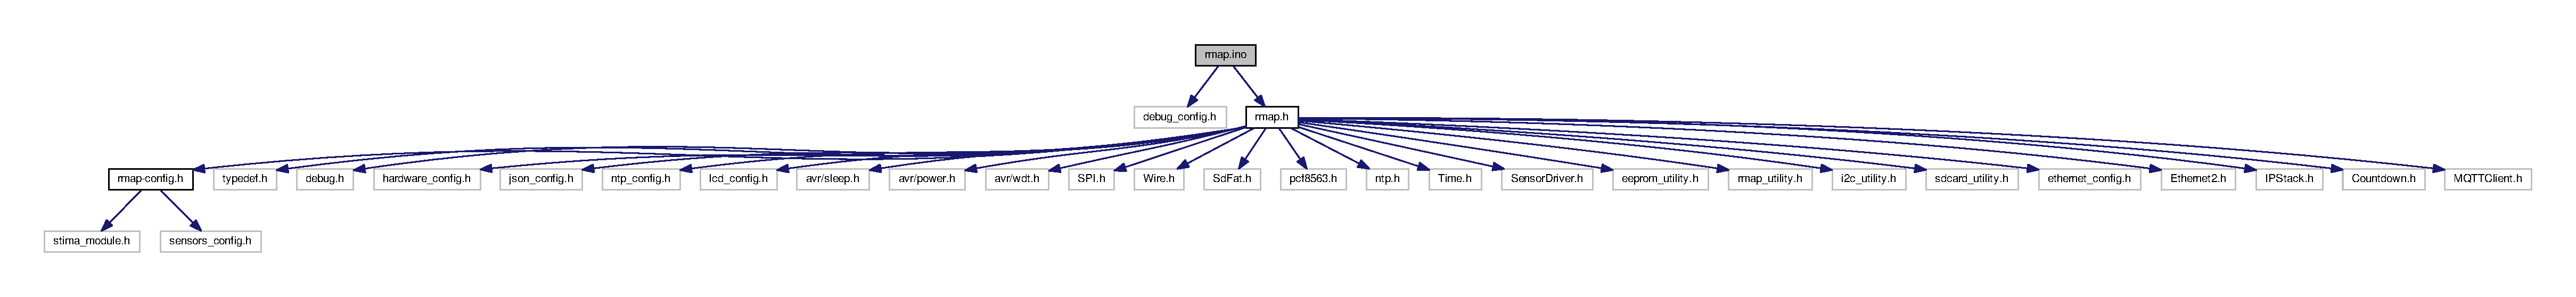
\includegraphics[width=350pt]{rmap_8ino__incl}
\end{center}
\end{figure}
\subsection*{Macros}
\begin{DoxyCompactItemize}
\item 
\mbox{\Hypertarget{rmap_8ino_a31fa5c36fa17c66feec7a67b76c3e786}\label{rmap_8ino_a31fa5c36fa17c66feec7a67b76c3e786}} 
\#define \hyperlink{rmap_8ino_a31fa5c36fa17c66feec7a67b76c3e786}{S\+E\+R\+I\+A\+L\+\_\+\+T\+R\+A\+C\+E\+\_\+\+L\+E\+V\+EL}~(R\+M\+A\+P\+\_\+\+S\+E\+R\+I\+A\+L\+\_\+\+T\+R\+A\+C\+E\+\_\+\+L\+E\+V\+EL)
\begin{DoxyCompactList}\small\item\em Serial debug level for this sketch. \end{DoxyCompactList}\item 
\mbox{\Hypertarget{rmap_8ino_acb771fe8deeaa2fee1ad327c0c1be34f}\label{rmap_8ino_acb771fe8deeaa2fee1ad327c0c1be34f}} 
\#define \hyperlink{rmap_8ino_acb771fe8deeaa2fee1ad327c0c1be34f}{L\+C\+D\+\_\+\+T\+R\+A\+C\+E\+\_\+\+L\+E\+V\+EL}~(R\+M\+A\+P\+\_\+\+L\+C\+D\+\_\+\+T\+R\+A\+C\+E\+\_\+\+L\+E\+V\+EL)
\begin{DoxyCompactList}\small\item\em L\+CD debug level for this sketch. \end{DoxyCompactList}\end{DoxyCompactItemize}
\subsection*{Functions}
\begin{DoxyCompactItemize}
\item 
void \hyperlink{rmap_8ino_a4fc01d736fe50cf5b977f755b675f11d}{setup} ()
\begin{DoxyCompactList}\small\item\em Arduino setup function. Init watchdog, hardware, debug, buffer and load configuration stored in E\+E\+P\+R\+OM. \end{DoxyCompactList}\item 
void \hyperlink{rmap_8ino_afe461d27b9c48d5921c00d521181f12f}{loop} ()
\begin{DoxyCompactList}\small\item\em Arduino loop function. First, initialize tasks and sensors, then execute the tasks and activates the power down if no task is running. \end{DoxyCompactList}\item 
void \hyperlink{rmap_8ino_afb98a0f07c30784284f48271ffe02b97}{init\+\_\+power\+\_\+down} (uint32\+\_\+t $\ast$time\+\_\+ms, uint32\+\_\+t debouncing\+\_\+ms)
\begin{DoxyCompactList}\small\item\em Enter power down mode. \end{DoxyCompactList}\item 
void \hyperlink{rmap_8ino_ad241cc00b1a92e6d85827df96778e442}{init\+\_\+buffers} ()
\begin{DoxyCompactList}\small\item\em Init buffers. \end{DoxyCompactList}\item 
void \hyperlink{rmap_8ino_ab4bf0a3d77da083f131d3fa35a37d2b1}{init\+\_\+tasks} ()
\begin{DoxyCompactList}\small\item\em Init tasks variable and state. \end{DoxyCompactList}\item 
void \hyperlink{rmap_8ino_ad8b80a0c08f928106018edd6ea435b95}{init\+\_\+pins} ()
\begin{DoxyCompactList}\small\item\em Init hardware pins. \end{DoxyCompactList}\item 
void \hyperlink{rmap_8ino_a2441543100bf8421f56edd622a2c1d9a}{init\+\_\+wire} ()
\begin{DoxyCompactList}\small\item\em Init wire (i2c) library and performs checks on the bus. \end{DoxyCompactList}\item 
void \hyperlink{rmap_8ino_a8eb9780a3438ec02c70314744f91f3c7}{init\+\_\+spi} ()
\begin{DoxyCompactList}\small\item\em Init S\+PI library. \end{DoxyCompactList}\item 
void \hyperlink{rmap_8ino_ab985cc69f5f573113405b4f118c96d33}{init\+\_\+rtc} ()
\begin{DoxyCompactList}\small\item\em Init R\+TC module. \end{DoxyCompactList}\item 
void \hyperlink{rmap_8ino_afceb890a6ab9be73cc5481369538c705}{init\+\_\+system} ()
\begin{DoxyCompactList}\small\item\em Init system. \end{DoxyCompactList}\item 
void \hyperlink{rmap_8ino_a980e73df66b14b1190bc25da430a4f12}{init\+\_\+wdt} (uint8\+\_\+t wdt\+\_\+timer)
\begin{DoxyCompactList}\small\item\em Init watchdog. \end{DoxyCompactList}\item 
void \hyperlink{rmap_8ino_ac74850003fab6eb3269bfe043d0f939c}{init\+\_\+sensors} ()
\begin{DoxyCompactList}\small\item\em Create and setup sensors. \end{DoxyCompactList}\item 
void \hyperlink{rmap_8ino_a1686e2719fa4a37ef933458673973d28}{set\+Next\+Time\+For\+Sensor\+Reading} (time\+\_\+t $\ast$next\+\_\+time)
\begin{DoxyCompactList}\small\item\em Calculate next hour, minute and second for sensors reading. \end{DoxyCompactList}\item 
bool \hyperlink{rmap_8ino_a9f5e5ca8c47d4536dd1805e89fbb7db2}{mqtt\+Connect} (char $\ast$username, char $\ast$password)
\begin{DoxyCompactList}\small\item\em Use a open tcp socket to connect to the mqtt server. \end{DoxyCompactList}\item 
bool \hyperlink{rmap_8ino_aa0d50218413a12917f8c70ef4e1e1e72}{mqtt\+Publish} (const char $\ast$topic, const char $\ast$message)
\begin{DoxyCompactList}\small\item\em Publish message on topic. \end{DoxyCompactList}\item 
void \hyperlink{rmap_8ino_a4fe2f970295d296f7f6725fe9e946933}{mqtt\+Rx\+Callback} (M\+Q\+T\+T\+::\+Message\+Data \&md)
\begin{DoxyCompactList}\small\item\em Register a receive callback for incoming mqtt message. \end{DoxyCompactList}\item 
void \hyperlink{rmap_8ino_a65b2dadc0411e43874ec8ed7f73bc62a}{print\+\_\+configuration} ()
\begin{DoxyCompactList}\small\item\em Print current configuration. \end{DoxyCompactList}\item 
void \hyperlink{rmap_8ino_a951e4934b8add405b8fe45417fc380f5}{set\+\_\+default\+\_\+configuration} ()
\begin{DoxyCompactList}\small\item\em Set default configuration to global configuration variable. \end{DoxyCompactList}\item 
void \hyperlink{rmap_8ino_afa979a8cb238fe81bf20654dfd6096ef}{save\+\_\+configuration} (bool is\+\_\+default)
\begin{DoxyCompactList}\small\item\em Save configuration to E\+E\+P\+R\+OM. \end{DoxyCompactList}\item 
void \hyperlink{rmap_8ino_a32a64a2800c724fb28e10636f2ec20b9}{load\+\_\+configuration} ()
\begin{DoxyCompactList}\small\item\em Load configuration from E\+E\+P\+R\+OM. \end{DoxyCompactList}\item 
char $\ast$ \hyperlink{rmap_8ino_a99f56f4c38f64be47b52818cbf57bb2d}{rpc\+\_\+process} (char $\ast$json)
\begin{DoxyCompactList}\small\item\em Process and execute a received Remote Procedure Call (R\+PC). Useful for configuration. \end{DoxyCompactList}\item 
void \hyperlink{rmap_8ino_a17374e428acd4fc86f2b8a8ede54deca}{rtc\+\_\+interrupt\+\_\+handler} ()
\begin{DoxyCompactList}\small\item\em Real Time Clock interrupt handler. \end{DoxyCompactList}\item 
void \hyperlink{rmap_8ino_a2f44f14407ed3f1ae93126c1533e697b}{supervisor\+\_\+task} ()
\begin{DoxyCompactList}\small\item\em Supervisor task. Manage R\+TC and N\+TP sync and open/close gsm and ethernet connection. \end{DoxyCompactList}\item 
void \hyperlink{rmap_8ino_a52f7fb7ebbd710f2a06b3f6e47c7e7e3}{rtc\+\_\+task} ()
\begin{DoxyCompactList}\small\item\em Real Time Clock task. Read R\+TC time and sync system time with it. \end{DoxyCompactList}\item 
void \hyperlink{rmap_8ino_a35c29025c5ef3d135b8c2b038be3f8df}{time\+\_\+task} ()
\begin{DoxyCompactList}\small\item\em Time task. Get time from N\+TP and sync R\+TC with it. \end{DoxyCompactList}\item 
void \hyperlink{rmap_8ino_abac8959915b759aa6429243ab9599ee3}{ethernet\+\_\+task} ()
\begin{DoxyCompactList}\small\item\em Ethernet task. Manage Ethernet operation. \end{DoxyCompactList}\item 
void \hyperlink{rmap_8ino_ad3efe51e17cb8205a24267c2992a12d4}{sensors\+\_\+reading\+\_\+task} ()
\begin{DoxyCompactList}\small\item\em Sensors reading Task. Read data from sensors. \end{DoxyCompactList}\item 
void \hyperlink{rmap_8ino_a1c6cee0cbd43bbe1215f13cab2434347}{data\+\_\+saving\+\_\+task} ()
\begin{DoxyCompactList}\small\item\em Data Saving Task. Save acquired sensors data on S\+D-\/\+Card. \end{DoxyCompactList}\item 
void \hyperlink{rmap_8ino_a161bca6629368a46242fec07a965966a}{mqtt\+\_\+task} ()
\begin{DoxyCompactList}\small\item\em M\+Q\+TT Task. \end{DoxyCompactList}\item 
bool \hyperlink{rmap_8ino_a21575354e8ec54fa31f581ed1838be79}{stream\+\_\+task} (Stream $\ast$stream, uint32\+\_\+t stream\+\_\+timeout, uint32\+\_\+t end\+\_\+task\+\_\+timeout)
\begin{DoxyCompactList}\small\item\em Stream Task. \end{DoxyCompactList}\end{DoxyCompactItemize}


\subsection{Function Documentation}
\mbox{\Hypertarget{rmap_8ino_a1c6cee0cbd43bbe1215f13cab2434347}\label{rmap_8ino_a1c6cee0cbd43bbe1215f13cab2434347}} 
\index{rmap.\+ino@{rmap.\+ino}!data\+\_\+saving\+\_\+task@{data\+\_\+saving\+\_\+task}}
\index{data\+\_\+saving\+\_\+task@{data\+\_\+saving\+\_\+task}!rmap.\+ino@{rmap.\+ino}}
\subsubsection{\texorpdfstring{data\+\_\+saving\+\_\+task()}{data\_saving\_task()}}
{\footnotesize\ttfamily void data\+\_\+saving\+\_\+task (\begin{DoxyParamCaption}\item[{void}]{ }\end{DoxyParamCaption})}



Data Saving Task. Save acquired sensors data on S\+D-\/\+Card. 

\begin{DoxyReturn}{Returns}
void. 
\end{DoxyReturn}
retry

fail

open sdcard file\+: today!

try to open file. if ok, write sensors data on it.

retry

fail

sdcard success

retry

fail \mbox{\Hypertarget{rmap_8ino_abac8959915b759aa6429243ab9599ee3}\label{rmap_8ino_abac8959915b759aa6429243ab9599ee3}} 
\index{rmap.\+ino@{rmap.\+ino}!ethernet\+\_\+task@{ethernet\+\_\+task}}
\index{ethernet\+\_\+task@{ethernet\+\_\+task}!rmap.\+ino@{rmap.\+ino}}
\subsubsection{\texorpdfstring{ethernet\+\_\+task()}{ethernet\_task()}}
{\footnotesize\ttfamily void ethernet\+\_\+task (\begin{DoxyParamCaption}\item[{void}]{ }\end{DoxyParamCaption})}



Ethernet task. Manage Ethernet operation. 

\begin{DoxyReturn}{Returns}
void. 
\end{DoxyReturn}
success

retry

fail

success

retry

fail \mbox{\Hypertarget{rmap_8ino_ad241cc00b1a92e6d85827df96778e442}\label{rmap_8ino_ad241cc00b1a92e6d85827df96778e442}} 
\index{rmap.\+ino@{rmap.\+ino}!init\+\_\+buffers@{init\+\_\+buffers}}
\index{init\+\_\+buffers@{init\+\_\+buffers}!rmap.\+ino@{rmap.\+ino}}
\subsubsection{\texorpdfstring{init\+\_\+buffers()}{init\_buffers()}}
{\footnotesize\ttfamily void init\+\_\+buffers (\begin{DoxyParamCaption}\item[{void}]{ }\end{DoxyParamCaption})}



Init buffers. 

\begin{DoxyReturn}{Returns}
void. 
\end{DoxyReturn}
\mbox{\Hypertarget{rmap_8ino_ad8b80a0c08f928106018edd6ea435b95}\label{rmap_8ino_ad8b80a0c08f928106018edd6ea435b95}} 
\index{rmap.\+ino@{rmap.\+ino}!init\+\_\+pins@{init\+\_\+pins}}
\index{init\+\_\+pins@{init\+\_\+pins}!rmap.\+ino@{rmap.\+ino}}
\subsubsection{\texorpdfstring{init\+\_\+pins()}{init\_pins()}}
{\footnotesize\ttfamily void init\+\_\+pins (\begin{DoxyParamCaption}\item[{void}]{ }\end{DoxyParamCaption})}



Init hardware pins. 

\begin{DoxyReturn}{Returns}
void. 
\end{DoxyReturn}
\mbox{\Hypertarget{rmap_8ino_afb98a0f07c30784284f48271ffe02b97}\label{rmap_8ino_afb98a0f07c30784284f48271ffe02b97}} 
\index{rmap.\+ino@{rmap.\+ino}!init\+\_\+power\+\_\+down@{init\+\_\+power\+\_\+down}}
\index{init\+\_\+power\+\_\+down@{init\+\_\+power\+\_\+down}!rmap.\+ino@{rmap.\+ino}}
\subsubsection{\texorpdfstring{init\+\_\+power\+\_\+down()}{init\_power\_down()}}
{\footnotesize\ttfamily void init\+\_\+power\+\_\+down (\begin{DoxyParamCaption}\item[{uint32\+\_\+t $\ast$}]{time\+\_\+ms,  }\item[{uint32\+\_\+t}]{debouncing\+\_\+ms }\end{DoxyParamCaption})}



Enter power down mode. 


\begin{DoxyParams}{Parameters}
{\em time\+\_\+ms} & pointer to a variable to save the last instant you entered power down. \\
\hline
{\em debouncing\+\_\+ms} & delay to power down. \\
\hline
\end{DoxyParams}
\begin{DoxyReturn}{Returns}
void. 
\end{DoxyReturn}
turn off brown-\/out enable in software \mbox{\Hypertarget{rmap_8ino_ab985cc69f5f573113405b4f118c96d33}\label{rmap_8ino_ab985cc69f5f573113405b4f118c96d33}} 
\index{rmap.\+ino@{rmap.\+ino}!init\+\_\+rtc@{init\+\_\+rtc}}
\index{init\+\_\+rtc@{init\+\_\+rtc}!rmap.\+ino@{rmap.\+ino}}
\subsubsection{\texorpdfstring{init\+\_\+rtc()}{init\_rtc()}}
{\footnotesize\ttfamily void init\+\_\+rtc (\begin{DoxyParamCaption}\item[{void}]{ }\end{DoxyParamCaption})}



Init R\+TC module. 

\begin{DoxyReturn}{Returns}
void. 
\end{DoxyReturn}
\mbox{\Hypertarget{rmap_8ino_ac74850003fab6eb3269bfe043d0f939c}\label{rmap_8ino_ac74850003fab6eb3269bfe043d0f939c}} 
\index{rmap.\+ino@{rmap.\+ino}!init\+\_\+sensors@{init\+\_\+sensors}}
\index{init\+\_\+sensors@{init\+\_\+sensors}!rmap.\+ino@{rmap.\+ino}}
\subsubsection{\texorpdfstring{init\+\_\+sensors()}{init\_sensors()}}
{\footnotesize\ttfamily void init\+\_\+sensors (\begin{DoxyParamCaption}\item[{void}]{ }\end{DoxyParamCaption})}



Create and setup sensors. 

\begin{DoxyReturn}{Returns}
void. 
\end{DoxyReturn}
read sensors configuration, create and setup \mbox{\Hypertarget{rmap_8ino_a8eb9780a3438ec02c70314744f91f3c7}\label{rmap_8ino_a8eb9780a3438ec02c70314744f91f3c7}} 
\index{rmap.\+ino@{rmap.\+ino}!init\+\_\+spi@{init\+\_\+spi}}
\index{init\+\_\+spi@{init\+\_\+spi}!rmap.\+ino@{rmap.\+ino}}
\subsubsection{\texorpdfstring{init\+\_\+spi()}{init\_spi()}}
{\footnotesize\ttfamily void init\+\_\+spi (\begin{DoxyParamCaption}\item[{void}]{ }\end{DoxyParamCaption})}



Init S\+PI library. 

\begin{DoxyReturn}{Returns}
void. 
\end{DoxyReturn}
\mbox{\Hypertarget{rmap_8ino_afceb890a6ab9be73cc5481369538c705}\label{rmap_8ino_afceb890a6ab9be73cc5481369538c705}} 
\index{rmap.\+ino@{rmap.\+ino}!init\+\_\+system@{init\+\_\+system}}
\index{init\+\_\+system@{init\+\_\+system}!rmap.\+ino@{rmap.\+ino}}
\subsubsection{\texorpdfstring{init\+\_\+system()}{init\_system()}}
{\footnotesize\ttfamily void init\+\_\+system (\begin{DoxyParamCaption}\item[{void}]{ }\end{DoxyParamCaption})}



Init system. 

\begin{DoxyReturn}{Returns}
void. 
\end{DoxyReturn}
main loop state \mbox{\Hypertarget{rmap_8ino_ab4bf0a3d77da083f131d3fa35a37d2b1}\label{rmap_8ino_ab4bf0a3d77da083f131d3fa35a37d2b1}} 
\index{rmap.\+ino@{rmap.\+ino}!init\+\_\+tasks@{init\+\_\+tasks}}
\index{init\+\_\+tasks@{init\+\_\+tasks}!rmap.\+ino@{rmap.\+ino}}
\subsubsection{\texorpdfstring{init\+\_\+tasks()}{init\_tasks()}}
{\footnotesize\ttfamily void init\+\_\+tasks (\begin{DoxyParamCaption}\item[{void}]{ }\end{DoxyParamCaption})}



Init tasks variable and state. 

\begin{DoxyReturn}{Returns}
void. 
\end{DoxyReturn}
\mbox{\Hypertarget{rmap_8ino_a980e73df66b14b1190bc25da430a4f12}\label{rmap_8ino_a980e73df66b14b1190bc25da430a4f12}} 
\index{rmap.\+ino@{rmap.\+ino}!init\+\_\+wdt@{init\+\_\+wdt}}
\index{init\+\_\+wdt@{init\+\_\+wdt}!rmap.\+ino@{rmap.\+ino}}
\subsubsection{\texorpdfstring{init\+\_\+wdt()}{init\_wdt()}}
{\footnotesize\ttfamily void init\+\_\+wdt (\begin{DoxyParamCaption}\item[{uint8\+\_\+t}]{wdt\+\_\+timer }\end{DoxyParamCaption})}



Init watchdog. 


\begin{DoxyParams}{Parameters}
{\em wdt\+\_\+timer} & a time value for init watchdog (W\+D\+T\+O\+\_\+xxxx). \\
\hline
\end{DoxyParams}
\begin{DoxyReturn}{Returns}
void. 
\end{DoxyReturn}
\mbox{\Hypertarget{rmap_8ino_a2441543100bf8421f56edd622a2c1d9a}\label{rmap_8ino_a2441543100bf8421f56edd622a2c1d9a}} 
\index{rmap.\+ino@{rmap.\+ino}!init\+\_\+wire@{init\+\_\+wire}}
\index{init\+\_\+wire@{init\+\_\+wire}!rmap.\+ino@{rmap.\+ino}}
\subsubsection{\texorpdfstring{init\+\_\+wire()}{init\_wire()}}
{\footnotesize\ttfamily void init\+\_\+wire (\begin{DoxyParamCaption}\item[{void}]{ }\end{DoxyParamCaption})}



Init wire (i2c) library and performs checks on the bus. 

\begin{DoxyReturn}{Returns}
void. 
\end{DoxyReturn}
\mbox{\Hypertarget{rmap_8ino_a32a64a2800c724fb28e10636f2ec20b9}\label{rmap_8ino_a32a64a2800c724fb28e10636f2ec20b9}} 
\index{rmap.\+ino@{rmap.\+ino}!load\+\_\+configuration@{load\+\_\+configuration}}
\index{load\+\_\+configuration@{load\+\_\+configuration}!rmap.\+ino@{rmap.\+ino}}
\subsubsection{\texorpdfstring{load\+\_\+configuration()}{load\_configuration()}}
{\footnotesize\ttfamily void load\+\_\+configuration (\begin{DoxyParamCaption}\item[{void}]{ }\end{DoxyParamCaption})}



Load configuration from E\+E\+P\+R\+OM. 

\begin{DoxyReturn}{Returns}
void. 
\end{DoxyReturn}
\mbox{\Hypertarget{rmap_8ino_afe461d27b9c48d5921c00d521181f12f}\label{rmap_8ino_afe461d27b9c48d5921c00d521181f12f}} 
\index{rmap.\+ino@{rmap.\+ino}!loop@{loop}}
\index{loop@{loop}!rmap.\+ino@{rmap.\+ino}}
\subsubsection{\texorpdfstring{loop()}{loop()}}
{\footnotesize\ttfamily void loop (\begin{DoxyParamCaption}{ }\end{DoxyParamCaption})}



Arduino loop function. First, initialize tasks and sensors, then execute the tasks and activates the power down if no task is running. 

\begin{DoxyReturn}{Returns}
void. 
\end{DoxyReturn}
\mbox{\Hypertarget{rmap_8ino_a161bca6629368a46242fec07a965966a}\label{rmap_8ino_a161bca6629368a46242fec07a965966a}} 
\index{rmap.\+ino@{rmap.\+ino}!mqtt\+\_\+task@{mqtt\+\_\+task}}
\index{mqtt\+\_\+task@{mqtt\+\_\+task}!rmap.\+ino@{rmap.\+ino}}
\subsubsection{\texorpdfstring{mqtt\+\_\+task()}{mqtt\_task()}}
{\footnotesize\ttfamily void mqtt\+\_\+task (\begin{DoxyParamCaption}\item[{void}]{ }\end{DoxyParamCaption})}



M\+Q\+TT Task. 

\begin{DoxyReturn}{Returns}
void. Read data stored on S\+D-\/\+Card and send it over M\+Q\+TT. 
\end{DoxyReturn}
retry

fail

try to open file. if ok, read ptr data.

retry

fail

found

not found (no sdcard error)\+: find it by starting from 1th January of this year

not found (sdcard error)

ptr not found. find it by searching in file name until today is reach. if there isn\textquotesingle{}t file, ptr\+\_\+time\+\_\+data is set to current date at 00\+:00\+:00 time.

ptr not found\+: set ptr to yesterday at 23\+:60-\/(uint8\+\_\+t)(readable\+\_\+configuration.\+report\+\_\+seconds / 60)\+:00 time.

ptr found\+: sooner or later the ptr will be set in any case

datafile read, reach eof and is today. E\+ND.

datafile read, reach eof and N\+OT is today. go to end of this day.

ptr data is found\+: send data saved on sdcard

ptr data is N\+OT found\+: sd card fault fallback\+: send last acquired sensor data

error\+: client not connected!

success

retry

fail

wait

ptr data is found\+: send data saved on sdcard

ptr data is N\+OT found\+: sd card fault fallback\+: send last acquired sensor data

E\+OF\+: End of File

mqtt json success

mqtt sdcard success

retry

fail

open the file that corresponds to the next data to send

open file for read data

error\+: file doesn\textquotesingle{}t exist but if is today, end.

error\+: file doesn\textquotesingle{}t exist and if it isn\textquotesingle{}t today, jump to next day and search in it

fail

set ptr 1 second more for send next data to current ptr

success

retry

fail \mbox{\Hypertarget{rmap_8ino_a9f5e5ca8c47d4536dd1805e89fbb7db2}\label{rmap_8ino_a9f5e5ca8c47d4536dd1805e89fbb7db2}} 
\index{rmap.\+ino@{rmap.\+ino}!mqtt\+Connect@{mqtt\+Connect}}
\index{mqtt\+Connect@{mqtt\+Connect}!rmap.\+ino@{rmap.\+ino}}
\subsubsection{\texorpdfstring{mqtt\+Connect()}{mqttConnect()}}
{\footnotesize\ttfamily bool mqtt\+Connect (\begin{DoxyParamCaption}\item[{char $\ast$}]{username,  }\item[{char $\ast$}]{password }\end{DoxyParamCaption})}



Use a open tcp socket to connect to the mqtt server. 


\begin{DoxyParams}{Parameters}
{\em $\ast$username} & Username of mqtt server \\
\hline
{\em $\ast$password} & Password of mqtt server \\
\hline
\end{DoxyParams}
\begin{DoxyReturn}{Returns}
true if connection was succesful, false otherwise. 
\end{DoxyReturn}
\mbox{\Hypertarget{rmap_8ino_aa0d50218413a12917f8c70ef4e1e1e72}\label{rmap_8ino_aa0d50218413a12917f8c70ef4e1e1e72}} 
\index{rmap.\+ino@{rmap.\+ino}!mqtt\+Publish@{mqtt\+Publish}}
\index{mqtt\+Publish@{mqtt\+Publish}!rmap.\+ino@{rmap.\+ino}}
\subsubsection{\texorpdfstring{mqtt\+Publish()}{mqttPublish()}}
{\footnotesize\ttfamily bool mqtt\+Publish (\begin{DoxyParamCaption}\item[{const char $\ast$}]{topic,  }\item[{const char $\ast$}]{message }\end{DoxyParamCaption})}



Publish message on topic. 


\begin{DoxyParams}{Parameters}
{\em $\ast$topic} & Topic for mqtt publish \\
\hline
{\em $\ast$message} & Message to be publish \\
\hline
\end{DoxyParams}
\begin{DoxyReturn}{Returns}
true if publish was succesful, false otherwise. 
\end{DoxyReturn}
\mbox{\Hypertarget{rmap_8ino_a4fe2f970295d296f7f6725fe9e946933}\label{rmap_8ino_a4fe2f970295d296f7f6725fe9e946933}} 
\index{rmap.\+ino@{rmap.\+ino}!mqtt\+Rx\+Callback@{mqtt\+Rx\+Callback}}
\index{mqtt\+Rx\+Callback@{mqtt\+Rx\+Callback}!rmap.\+ino@{rmap.\+ino}}
\subsubsection{\texorpdfstring{mqtt\+Rx\+Callback()}{mqttRxCallback()}}
{\footnotesize\ttfamily void mqtt\+Rx\+Callback (\begin{DoxyParamCaption}\item[{M\+Q\+T\+T\+::\+Message\+Data \&}]{md }\end{DoxyParamCaption})}



Register a receive callback for incoming mqtt message. 


\begin{DoxyParams}{Parameters}
{\em \&md} & Received data structure \\
\hline
\end{DoxyParams}
\begin{DoxyReturn}{Returns}
void. 
\end{DoxyReturn}
\mbox{\Hypertarget{rmap_8ino_a65b2dadc0411e43874ec8ed7f73bc62a}\label{rmap_8ino_a65b2dadc0411e43874ec8ed7f73bc62a}} 
\index{rmap.\+ino@{rmap.\+ino}!print\+\_\+configuration@{print\+\_\+configuration}}
\index{print\+\_\+configuration@{print\+\_\+configuration}!rmap.\+ino@{rmap.\+ino}}
\subsubsection{\texorpdfstring{print\+\_\+configuration()}{print\_configuration()}}
{\footnotesize\ttfamily void print\+\_\+configuration (\begin{DoxyParamCaption}\item[{void}]{ }\end{DoxyParamCaption})}



Print current configuration. 

\begin{DoxyReturn}{Returns}
void. 
\end{DoxyReturn}
\mbox{\Hypertarget{rmap_8ino_a99f56f4c38f64be47b52818cbf57bb2d}\label{rmap_8ino_a99f56f4c38f64be47b52818cbf57bb2d}} 
\index{rmap.\+ino@{rmap.\+ino}!rpc\+\_\+process@{rpc\+\_\+process}}
\index{rpc\+\_\+process@{rpc\+\_\+process}!rmap.\+ino@{rmap.\+ino}}
\subsubsection{\texorpdfstring{rpc\+\_\+process()}{rpc\_process()}}
{\footnotesize\ttfamily char$\ast$ rpc\+\_\+process (\begin{DoxyParamCaption}\item[{char $\ast$}]{json }\end{DoxyParamCaption})}



Process and execute a received Remote Procedure Call (R\+PC). Useful for configuration. 


\begin{DoxyParams}{Parameters}
{\em $\ast$json} & message in json text format \\
\hline
\end{DoxyParams}
\begin{DoxyReturn}{Returns}
pointer to R\+PC response. 
\end{DoxyReturn}
\mbox{\Hypertarget{rmap_8ino_a17374e428acd4fc86f2b8a8ede54deca}\label{rmap_8ino_a17374e428acd4fc86f2b8a8ede54deca}} 
\index{rmap.\+ino@{rmap.\+ino}!rtc\+\_\+interrupt\+\_\+handler@{rtc\+\_\+interrupt\+\_\+handler}}
\index{rtc\+\_\+interrupt\+\_\+handler@{rtc\+\_\+interrupt\+\_\+handler}!rmap.\+ino@{rmap.\+ino}}
\subsubsection{\texorpdfstring{rtc\+\_\+interrupt\+\_\+handler()}{rtc\_interrupt\_handler()}}
{\footnotesize\ttfamily void rtc\+\_\+interrupt\+\_\+handler (\begin{DoxyParamCaption}\item[{void}]{ }\end{DoxyParamCaption})}



Real Time Clock interrupt handler. 

\begin{DoxyReturn}{Returns}
void. 
\end{DoxyReturn}
\mbox{\Hypertarget{rmap_8ino_a52f7fb7ebbd710f2a06b3f6e47c7e7e3}\label{rmap_8ino_a52f7fb7ebbd710f2a06b3f6e47c7e7e3}} 
\index{rmap.\+ino@{rmap.\+ino}!rtc\+\_\+task@{rtc\+\_\+task}}
\index{rtc\+\_\+task@{rtc\+\_\+task}!rmap.\+ino@{rmap.\+ino}}
\subsubsection{\texorpdfstring{rtc\+\_\+task()}{rtc\_task()}}
{\footnotesize\ttfamily void rtc\+\_\+task (\begin{DoxyParamCaption}\item[{void}]{ }\end{DoxyParamCaption})}



Real Time Clock task. Read R\+TC time and sync system time with it. 

\begin{DoxyReturn}{Returns}
void. 
\end{DoxyReturn}
\mbox{\Hypertarget{rmap_8ino_afa979a8cb238fe81bf20654dfd6096ef}\label{rmap_8ino_afa979a8cb238fe81bf20654dfd6096ef}} 
\index{rmap.\+ino@{rmap.\+ino}!save\+\_\+configuration@{save\+\_\+configuration}}
\index{save\+\_\+configuration@{save\+\_\+configuration}!rmap.\+ino@{rmap.\+ino}}
\subsubsection{\texorpdfstring{save\+\_\+configuration()}{save\_configuration()}}
{\footnotesize\ttfamily void save\+\_\+configuration (\begin{DoxyParamCaption}\item[{bool}]{is\+\_\+default }\end{DoxyParamCaption})}



Save configuration to E\+E\+P\+R\+OM. 


\begin{DoxyParams}{Parameters}
{\em is\+\_\+default} & if true save default configuration; if false save current configuration. \\
\hline
\end{DoxyParams}
\begin{DoxyReturn}{Returns}
void. 
\end{DoxyReturn}
\mbox{\Hypertarget{rmap_8ino_ad3efe51e17cb8205a24267c2992a12d4}\label{rmap_8ino_ad3efe51e17cb8205a24267c2992a12d4}} 
\index{rmap.\+ino@{rmap.\+ino}!sensors\+\_\+reading\+\_\+task@{sensors\+\_\+reading\+\_\+task}}
\index{sensors\+\_\+reading\+\_\+task@{sensors\+\_\+reading\+\_\+task}!rmap.\+ino@{rmap.\+ino}}
\subsubsection{\texorpdfstring{sensors\+\_\+reading\+\_\+task()}{sensors\_reading\_task()}}
{\footnotesize\ttfamily void sensors\+\_\+reading\+\_\+task (\begin{DoxyParamCaption}\item[{void}]{ }\end{DoxyParamCaption})}



Sensors reading Task. Read data from sensors. 

\begin{DoxyReturn}{Returns}
void. 
\end{DoxyReturn}
success

retry

fail

end

success

retry

fail

not end

next sensor

end

first time\+: read ptr data from sdcard

other time\+: save data to sdcard \mbox{\Hypertarget{rmap_8ino_a951e4934b8add405b8fe45417fc380f5}\label{rmap_8ino_a951e4934b8add405b8fe45417fc380f5}} 
\index{rmap.\+ino@{rmap.\+ino}!set\+\_\+default\+\_\+configuration@{set\+\_\+default\+\_\+configuration}}
\index{set\+\_\+default\+\_\+configuration@{set\+\_\+default\+\_\+configuration}!rmap.\+ino@{rmap.\+ino}}
\subsubsection{\texorpdfstring{set\+\_\+default\+\_\+configuration()}{set\_default\_configuration()}}
{\footnotesize\ttfamily void set\+\_\+default\+\_\+configuration (\begin{DoxyParamCaption}\item[{void}]{ }\end{DoxyParamCaption})}



Set default configuration to global configuration variable. 

\begin{DoxyReturn}{Returns}
void. 
\end{DoxyReturn}
\mbox{\Hypertarget{rmap_8ino_a1686e2719fa4a37ef933458673973d28}\label{rmap_8ino_a1686e2719fa4a37ef933458673973d28}} 
\index{rmap.\+ino@{rmap.\+ino}!set\+Next\+Time\+For\+Sensor\+Reading@{set\+Next\+Time\+For\+Sensor\+Reading}}
\index{set\+Next\+Time\+For\+Sensor\+Reading@{set\+Next\+Time\+For\+Sensor\+Reading}!rmap.\+ino@{rmap.\+ino}}
\subsubsection{\texorpdfstring{set\+Next\+Time\+For\+Sensor\+Reading()}{setNextTimeForSensorReading()}}
{\footnotesize\ttfamily void set\+Next\+Time\+For\+Sensor\+Reading (\begin{DoxyParamCaption}\item[{time\+\_\+t $\ast$}]{next\+\_\+time }\end{DoxyParamCaption})}



Calculate next hour, minute and second for sensors reading. 


\begin{DoxyParams}{Parameters}
{\em $\ast$next\+\_\+time} & Pointer to next scheduled time for sensors reading \\
\hline
\end{DoxyParams}
\begin{DoxyReturn}{Returns}
void. 
\end{DoxyReturn}
\mbox{\Hypertarget{rmap_8ino_a4fc01d736fe50cf5b977f755b675f11d}\label{rmap_8ino_a4fc01d736fe50cf5b977f755b675f11d}} 
\index{rmap.\+ino@{rmap.\+ino}!setup@{setup}}
\index{setup@{setup}!rmap.\+ino@{rmap.\+ino}}
\subsubsection{\texorpdfstring{setup()}{setup()}}
{\footnotesize\ttfamily void setup (\begin{DoxyParamCaption}{ }\end{DoxyParamCaption})}



Arduino setup function. Init watchdog, hardware, debug, buffer and load configuration stored in E\+E\+P\+R\+OM. 

\begin{DoxyReturn}{Returns}
void. 
\end{DoxyReturn}
\mbox{\Hypertarget{rmap_8ino_a21575354e8ec54fa31f581ed1838be79}\label{rmap_8ino_a21575354e8ec54fa31f581ed1838be79}} 
\index{rmap.\+ino@{rmap.\+ino}!stream\+\_\+task@{stream\+\_\+task}}
\index{stream\+\_\+task@{stream\+\_\+task}!rmap.\+ino@{rmap.\+ino}}
\subsubsection{\texorpdfstring{stream\+\_\+task()}{stream\_task()}}
{\footnotesize\ttfamily bool stream\+\_\+task (\begin{DoxyParamCaption}\item[{Stream $\ast$}]{stream,  }\item[{uint32\+\_\+t}]{stream\+\_\+timeout,  }\item[{uint32\+\_\+t}]{end\+\_\+task\+\_\+timeout }\end{DoxyParamCaption})}



Stream Task. 


\begin{DoxyParams}{Parameters}
{\em $\ast$stream} & Pointer to stream \\
\hline
{\em stream\+\_\+timeout} & Timeout for stream \\
\hline
{\em end\+\_\+task\+\_\+timeout} & Timeout for deactivate task after last received bytes Read a stream and process Remote Procedure Call data. \\
\hline
\end{DoxyParams}
\begin{DoxyReturn}{Returns}
true if end\+\_\+task\+\_\+timeout was elapsed, false otherwise. 
\end{DoxyReturn}
\mbox{\Hypertarget{rmap_8ino_a2f44f14407ed3f1ae93126c1533e697b}\label{rmap_8ino_a2f44f14407ed3f1ae93126c1533e697b}} 
\index{rmap.\+ino@{rmap.\+ino}!supervisor\+\_\+task@{supervisor\+\_\+task}}
\index{supervisor\+\_\+task@{supervisor\+\_\+task}!rmap.\+ino@{rmap.\+ino}}
\subsubsection{\texorpdfstring{supervisor\+\_\+task()}{supervisor\_task()}}
{\footnotesize\ttfamily void supervisor\+\_\+task (\begin{DoxyParamCaption}\item[{void}]{ }\end{DoxyParamCaption})}



Supervisor task. Manage R\+TC and N\+TP sync and open/close gsm and ethernet connection. 

\begin{DoxyReturn}{Returns}
void. 
\end{DoxyReturn}
need ntp sync ?

enable hardware related tasks for connect

success

reset time task for doing ntp sync

doing other operations...

error

retry

fail

enable time task

success

success or error

reinit lcd display \mbox{\Hypertarget{rmap_8ino_a35c29025c5ef3d135b8c2b038be3f8df}\label{rmap_8ino_a35c29025c5ef3d135b8c2b038be3f8df}} 
\index{rmap.\+ino@{rmap.\+ino}!time\+\_\+task@{time\+\_\+task}}
\index{time\+\_\+task@{time\+\_\+task}!rmap.\+ino@{rmap.\+ino}}
\subsubsection{\texorpdfstring{time\+\_\+task()}{time\_task()}}
{\footnotesize\ttfamily void time\+\_\+task (\begin{DoxyParamCaption}\item[{void}]{ }\end{DoxyParamCaption})}



Time task. Get time from N\+TP and sync R\+TC with it. 

\begin{DoxyReturn}{Returns}
void. 
\end{DoxyReturn}
success

retry

fail\+: use old rtc time

success\+: 946684800 seconds for 01/01/2000 00\+:00\+:00

retry

fail

retry

fail 
%--- End generated contents ---

% Index
\backmatter
\newpage
\phantomsection
\clearemptydoublepage
\addcontentsline{toc}{chapter}{Index}
\printindex

\end{document}
